\documentclass[journal,onecolumn]{IEEEtran}

\usepackage{cite}

% *** GRAPHICS RELATED PACKAGES ***
%
\ifCLASSINFOpdf
  \usepackage[pdftex]{graphicx}
  \graphicspath{{../img/}}
\else
  \usepackage[dvips]{graphicx}
  \graphicspath{{../img/}}
\fi

% *** SPECIALIZED LIST PACKAGES ***
%
\usepackage{algorithmic}

\usepackage{array}

% *** PDF, URL AND HYPERLINK PACKAGES ***
%
\usepackage{url}

% correct bad hyphenation here
\hyphenation{op-tical net-works}

\begin{document}

\title{Volunteers in the Clouds: A Web Based Architecture to Harness Volunteer Computational Resources 
for Low Cost Distributed Evolutionary Computation }
% The word massive in the title is giving us problems.
% Why not change it to something about sharing resources?.
% Also lets not forget about volunteers, they can be a resource too
% and they cannot be replaced by any super computer

%  I propose something like:
% A Web Based Architecture to Harness Volunteer Computational Resources 
% for Low Cost Distributed Evolutionary Computation

% Some keywords missing: Cloud, Asynchronous, Pool-Based, Javascript-Based
% Open Source software.
% Lets not forget this issue is about software.

\author{Juan-J.~Merelo*$^1$, Mario Garc\'ia-Valdez$^2$, Pedro A. Castillo$^1$, Pablo Garc\'ia-S\'anchez$^1$, P. de las Cuevas*$^1$, Nuria Rico$^3$
\thanks{Manuscript submitted for review on \today.}%
\thanks{$^1$Dept. of Computer Architecture and Technology and CITIC University of Granada}%
\thanks{$^2$Dept. of Graduate Studies at Instituto Tecnol\'ogico de Tijuana}%
\thanks{$^3$Dept. of Statistics and Operational Research University of Granada}%
\thanks{E-mail addresses: {\tt jmerelo@ugr.es}, {\tt
    mario@tectijuana.edu.mx}, {\tt pacv@ugr.es}, {\tt pablogarcia@ugr.es},{\tt nrico@ugr.es}}%
\thanks{*Corresponding author.}%
}

\maketitle

\begin{abstract}
Volunteer computing is extensively used 
% (Paloma) Adverbs are always written before verbs, check this throughout the text
in science and industry, but it
still has a long way to go in order to become
% (Paloma) I would propose "a long way to go in order to become"
 a mainstream
technology in the same way the cloud technologies in general have. The
lack of % (Paloma) Add "both" here to better complete the sentence
general purpose and open source tools with built-in analytics 
% (Paloma) "built-in" is an adjective and, as such, has to be written before names
could be one of the reasons of why this is so, as well as the lack of
proofs of concept. That is why in this paper we present {\sf NodIO}, a
framework used to create client-server architectures for distributed
evolutionary algorithms, entirely written  % (Paloma) Adverb. I would also add an "and" after the comma
in JavaScript, which needs
minimal server support to work and is able to support persistent,
asynchronous, distributed evolutionary algorithms running in the
browser, as well as any other client consuming its REST application
programming interface.  The architecture, along with some initial
results on the expected performance and scaling behavior when the
number of users is increased is presented. We also use
the algorithm data to find out what kind of patterns the user behavior
follow by examining the resources they devote to our experiment, and
try to fit them to some statistical distribution to create the bases
of a model of user behavior in volunteer computing experiments of this
kind that can be used by researchers to predict its performance. 
In general, our experiments prove, first, that {\sf NodIO} is a flexible and
low-overhead platform to perform distributed computation experiments
that include volunteers, and then that user behavior follows some patterns,
and, thus, are amenable to a model.
\end{abstract}

% Work in progress..
%Volunteer computing is used routinely in science and industry, but it
%still has a long way to go if it is going to become a mainstream technology 
%in the same way the cloud technologies in general have. In one hand, projects 
%lack special purpose and open source tools with analytics builtin and
%in the other there are still barriers that keep users from sharing their computing 
%resources like the need to install software applications or plugins in order 
%to cooperate. That is why in this paper we present {\sf NodIO}, a client-server
%architecture for distributed
%evolutionary algorithms, written entirely in JavaScript, which needs
%minimal server support to work and is able to support persistent,
%asynchronous, distributed evolutionary algorithms running in the
%browser.  The architecture, along with some initial results on the
%expected performance and scaling
%behavior is presented. We also use the algorithm data to
%find out what kind of patterns the user behavior follow and try to fit
%them to some statistical distribution.



\begin{IEEEkeywords}
Evolutionary algorithms, evolutionary computation, distributed computing, internet computing,
social networks, volunteer computing, metacomputing, performance evaluation.
\end{IEEEkeywords}

%---------------------------------------------------------------
\section{Introduction}

\IEEEPARstart{N}{owadays} there is a big and increasing number of
distributed evolutionary computation software frameworks available on
the market, usually as open source systems \cite{Parejo12Survey}. Most of these systems have 
two features: they are {\em desktop} applications, that is, they must
be compiled or run directly on the operating system layer and, second,
they assume that the nodes that are going to run the system are under
the control of developers or they at least have access to them.

There is, then, space for systems that do not make any of these
assumptions, such as the one presented in this paper, which will be
provisionally named {\sf NodIO}. {\sf NodIO} is basically
% (Paloma) Is the "first" word really needed? 
% (Mario) I guess is more related to fundamentally or primarily but "basically" sounds better
a two tier client/server 
application, in which clients can run on a browser. 
Therefore, they can
% (Paloma) be embedded in?
be embedded in any web-enabled device, including many over which 
developers have no control.

Some time ago, our group faced the problem of diminishing funds for
buying new hardware. This was aggravated by the increasing maintenance costs and
extended downtime resulting from the continuous failures of existing
clusters.
Considering this, we leveraged 
% (Paloma) What 'something' did you leverage?
our experience in the design of web
applications, including JavaScript, since their inception and other
volunteer and
unconventional distributed evolutionary computing systems to 
design and release a new free framework that would allow anyone to
create a volunteer distributed EC experiment using cloud resources as
servers and browsers as clients.
% (Paloma) I think you should rewrite this whole sentence.
% For starters, focus in that you "leveraged" the problem through your deeply knowledge of... this and that. And "Thus/Then/Therefore", you decided... 
% (Mario) We leverage our experience in blah blah to design
% (Paloma) It may be... guess I was thinking in the noun, not in the transitive verb

%PABLO: He añadido el siguiente párrafo para el issue #31
There exist other volunteer frameworks written in compiled languages,
such as C++ or Java, that can achieve better performance than
JavaScript. However, one of the advantages of our system is that
clients do not need to install anything in their machines, they just
need to open a web page  
% Somewhat redundant 
% Javascript is the only language that can be executed in this way without any installation, 
% also removed the default, redundant with next sentence
in a compatible browser, such as Chrome, Safari or Firefox, which are
available in almost every desktop or mobile device. Other advantage is
that the source code can be directly examined by volunteers, because it is not
compiled as other options such as Java Applets, ActionScript or
ActiveX.
% (Paloma) Brackets not really needed here
Also, as we discuss in this paper, it can provide some extra
features such as enhanced security or operating system independence. 

%PABLO: hay que enlazar con el siguiente párrafo
%Desktop clients have the same issues as any 
%volunteer computing system, including our % (Paloma) their?
% own: these issues are
%related to security as well as
%safety, which introduce 

When developing volunteer based systems, designers must
also consider the whole {\em social} aspect in the design, with
issues related to security, trust and privacy among others. 
The computing system becomes a {\em techno-social system} \cite{vespignani2009predicting}.  
% (Paloma) Is the social aspect related to the word "safety"? It's not completely clear.
%a {\em social} aspect to the design of a
%computing system that makes it a {\em techno-social system}
In this paper, our intention is to
present the {\sf NodIO} framework and analyze it from two different
angles: the purely technical angle, including the decisions that went
into its features, and the social angle, to account on how the persons
that voluntarily choose to enter the web page running the system
determine its performance and how it can be modeled and, eventually,
predicted.

The rest of the paper is organized as follows: Next we present the
state of the art (Section \ref{sec:soa}) in web-based distributed
computational systems along with attempts to predict and model its behavior. 
Then, a detailed description of the proposed system is presented
in Section \ref{sec:description}, followed by the baseline experiments
in Section \ref{sec:experiments}, and experiments using a new client
architecture that uses web workers in Section \ref{sec:w2}.
Finally, conclusions and future lines of work are presented in Section
\ref{sec:conclusion}. 

%---------------------------------------------------------------
\section{State of the art}
\label{sec:soa}

The web used as a resource for distributed computing has a
long history, and almost since the beginning it was used for
evolutionary computation even before JavaScript was
introduced as a browser-based scripting language in 1997. Before that
time other technologies,
 including Flash animations and VBScript, ActiveX or Java applets were
used; for instance, Java was pointed out in \cite{soares1998get} as a
``language for the
internet'', providing some advantages such as multi-architecture compatibility or
security mechanisms, and was proposed in \cite{chandy1996world} as the
basis for the creation of a world-wide peer to peer system using compiled Java
programs. The ATLAS system
\cite{Baldeschwieler:1996:TIG:504450.504482} also used Java together
with another language called Cilk; all these papers indicated that
the introduction of an architecture-independent system such as the
Java virtual machine opened the doors for ultrascale, Internet-wide,
metacomputers. This paper also establishes the desirable features of
any {\em global computing} infrastructure, that can also be applied to
distributed evolutionary computation experiments that rely on
volunteer computing: scalability, heterogeneity, fault tolerance,
adaptive parallelism, safety, anonymity, hierarchy, ease of use, and
reasonable performance. But hierarchy, this is, the capability of
preferentially using resources in the same organization, is a feature
that could be either disregarded or included within adaptivity, which
leaves us with eight desirable properties. 
% (Paloma) Re-write. For example, "But is hierarchy, this is, the
% capability of preferentially using resources in the same
% organization, the one that could be either disregarded or included
% in adaptivity, which leaves us with eight desirable properties." 
% (Paloma) And I re-wrote what I proposed yesterday.
% thanks :-) -JJ

The fulfillment of these properties could be achieved by using any of the
languages and associated technologies, mentioned above, provided that the user had
installed the required virtual machine plugin first. 
% (Paloma) These should be separate sentences
However, embedding a
distributed computation client in the browser has the advantage of
providing a single and universal way of accessing resources via an
URI, something that is not guaranteed by using desktop
applications. Baratloo et al. tried in 1996 to create a system with
the aforementioned qualities called {\em Charlotte}
\cite{baratloo1996charlotte}. This system, which implemented a
distributed shared memory, was inspired by a previous work
on parallel computing systems PVM and MPI and solved most of the issues by
using the Java virtual machine embedded in the browser,
which provided
security to the user, uniformity of computing environment
independently of the operating system, and access to a common data store in the
server. Since the Java virtual machine is a sandbox, it is safe to the user
and as it runs compiled bytecode it also guarantees a certain level of
performance.
Other issues such as scheduling, which are related to adaptive 
parallelism, were solved on the server. This
paper was later extended and published in a journal in 1999
\cite{baratloo1999charlotte}, but it is interesting to note that,
even in the early stages of the web, the possibility of
% (Paloma) Re-write. For example, "but it is interesting to note that, even in the early stages of the web, the possibility of..."
browser-based distributed computing was already researched. 


Other systems, like JET, proposed by Soares et
al. \cite{soares1998get}, also used Java. JET supports
the execution of parallel applications over the Internet and features
a comprehensive statistics collection subsystem, enabling its use for science, %(Mario) Was easier to change "allowing"
since it allows % (Paloma) Use synonyms, like "yield" or "permit" 
the collection of algorithm analytics by the
experiment designer, unlike the other systems mentioned
above. Other proposals contemporary to JET, such as {\em SuperWeb}
\cite{alexandrov1997superweb} are roughly a translation of classical
distribution techniques, with overly complicated architectures that include
brokers for resource discovery. SuperWeb is focused
% (Paloma) Careful with starting using plural ("Other proposals", "are") and continuig with singular. If you are referring to "SuperWeb", change "It" for "SuperWeb"
, however, in solving the
issues involved in browser-based computing and also in making a system
that is able to work across different types of computers, mentioning
SPARCstations and PCs with Windows-95. Interestingly enough, this
paper incorporates a discussion on the economic model, paving the way
for the for-profit distributed computing systems that arose later on. 
On the other hand, the potential for volunteer computing using
browsers was realized
later on \cite{sarmenta-bayanihan} as well as the potential of
user misconduct when having access to the source code.
% (Paloma) I think this sentence is extremely informal
\cite{sarmenta-sabotagetolerance}. However, these early efforts by
Sarmenta once again used Java and not JavaScript, making them % (Paloma) making them
less widespread.

The main problem with Java and all the other browser-embedded
technologies is that they are not {\em universal} in the
sense than an extra component, namely, the Java virtual machine or another
virtual environment has to be installed in the browser.
Also these virtual environments have become targets of malicious attacks; 
for instance numerous vulnerabilities have been discovered in 
the proprietary Adobe Flash runtime environment and
video player \cite{ford2009analyzing,watanabe2010new}. The need for
these additional environments has been mitigated with the
adoption of the HTML5 standard \cite{anthes2012html5}.
JavaScript \cite{flanagan2006javascript}, however, has become a set of standards
\cite{ECMA-262} that include the language and its components. Since
early on, it was adopted by the industry and also by scientists,
who used them for creating an EA on
the browser as early as 1998 \cite{jj-ppsn98}.

JavaScript can be used either for unwitting
\cite{unwitting-ec} or volunteer 
\cite{langdon:2005:metas,gecco07:workshop:dcor} distributed
evolutionary computation and it has been used ever since by several
authors, including more recent efforts
\cite{Desell:2008:AHG:1389095.1389273,duda2013distributed,DBLP:journals/corr/abs-0801-1210} 
that even
used the client's GPU \cite{duda2013gpu} or create an object-oriented
framework for evolution in the browser \cite{EvoStar2014:jsEO}. Many other researchers have
used Java \cite{chong:1999:jDGPi} and others have gone away from the
server-based paradigm to embrace peer to peer systems
\cite{jin2006constructing,10.1109/ICICSE.2008.99,DBLP:conf/3pgcic/GuervosMFEL12}. These computing
platforms avoid single points of failure (the server) but, since they
need a certain amount of infrastructure installed to start, the
threshold to join them is much lower.

Recent works propose the use of cloud computing services for the components of
client-server distributed EAs. Cloud resources
can reduce operational costs by outsourcing both hardware and software maintenance
to the cloud provider. Another advantage is that they enable the provisioning of computing resources beyond what
is available in most laboratories, allowing researches to
scale algorithms at reasonable costs. Researchers have proposed the use of
public clouds such as Amazon EC2 \cite{CloudScale}, Google App Engine\cite{di2013towards},
and DropBox~\cite{mericloud}. The use of JavaScript to implement
server side components
gives software developers certain advantages in the cloud
paradigm, since it is a first-class citizen
in most Platforms as a Service (PaaS) products as the {\tt Node.js} framework is supported by most of them. \cite{wood13:nodejs:paas}. Many web services
have native JavaScript libraries too, and also use the JSON (JavaScript Object Notation) format for data interchange. Another advantage is that
developers can use the same software tools for both client and server
side development.

JavaScript is also compatible with the functional programming paradigm \cite{Cousineau1998,MacLennan1990,Thompson1996}.
According to \cite{swanresearch2015}, the benefit of using this kind of paradigm in
metaheuristics optimization is that it allows an improvement in communicability,
reproductibility, interoperability, automated assembly, knowledge engineering
and efficiency.

In the work presented in this paper, JavaScript has been used throughout the full
stack, which has the advantage of using the self-same lines of code for
writing an evolutionary algorithm for the
desktop or command line and browser clients, both based in the EC
library {\sf NodEO} \cite{DBLP:conf/gecco/GuervosVGES14}. This saves time 
when writing code and leverages 
the expertise acquired
% (Paloma) Not sure if "acquired" should be written before "expertise"... sounds better to me, anyways
 in the library itself. 

On the other hand, we are also interested in measuring the performance
of volunteer computing systems, an area in which there have been
relatively few efforts.
There were some initial attempts to avoid the differences in performance
that could be obtained from volunteers  by making
the algorithm adaptive to the kind of resources allotted to it
\cite{milani2004online}, which is actually not such a big problem in
algorithms such as the EA that can easily be
parallelized via population splitting or farming out evaluations to all
the nodes available. Lately, several approaches have focused on the
fault-tolerance of volunteer algorithms
\cite{gonzalez2010characterizing} which it can, of course, be studied in
the more general context of distributed computing 
\cite{nogueras2015studying} or including it in a more general study of the
performance of the EA itself
\cite{DBLP:journals/gpem/LaredoBGVAGF14}.

On the other hand, measuring the performance of the resulting metacomputer
involves understanding the dynamics of this kind of systems. Initial
work was done for peer to peer systems by Stutzbach et
al. \cite{stutzbach2006understanding} and extended to volunteer
computing by Laredo et al. \cite{churn08,laredo2008rcp}. 
%But the raw material of           
%volunteer computing, % (Paloma) Whith regard to?  Maybe it was colloquial/analogy
But some of the essential metrics in volunteer computing like the
number of users or the time spent by every one in the
computation in browser-based volunteer computing experiments, have
only been studied in a limited way in 
\cite{DBLP:journals/gpem/LaredoBGVAGF14} on the basis of a single
run. Studies using volunteer computing platforms such as SETI@home
\cite{javadi2009mining} found out that the Weibull, log-normal and
Gamma distribution 
modeled quite well the availability of resources in several clusters
of that framework; the shape of those distributions is a skewed bell
with more resources in the {\em low} areas than in the high areas:
there are many users that give a small amount of cycles, while there
are just a few that give many cycles. This is in concordance with the
results obtained in \cite{agajaj}. Although SETI@home works
at a larger scale in both quantity of volunteers and the scope of projects, 
our initial tests indicate that
this kind of distribution might be the most appropriate to describe
user participation in several different metrics. However, in this
paper we will perform different experiments in different setups and
will try to come up with a more precise model. Next we describe the
system itself.


As far as we know, this paper presents one of the few experiments using % (Paloma) Change to "which" in order to not repeating "that" all the time
computational resources that are as dissimilar as smartphones and
powerful laptops 
or workstation computers in a research center. 
%The methodology used
% (Paloma) I would say "the used methodology"
The algorithms used, as well as the methodology 
for gathering resources will be described next, 
together with the results obtained in this initial setup.
%---------------------------------------------------------------
\section{Description of the framework}
\label{sec:description}

In general, a distributed volunteer-based evolutionary computation
system based on the browser is simply a client-server system
whose client is, or it can be, embedded in the browser via
JavaScript. Since JavaScript is  the only language that is present
across all browsers, the choice was quite clear. Even so, there might
be some issues with the performance of the language itself; which % (Paloma) I recommend the use of "which" here
 is
why we have made a comparison between JavaScript and other languages
\cite{2015arXiv151101088M}. The results of this work show that JavaScript can be
faster than compiled languages such as Scala and, in any case, it provides
a performance that is comparable to other languages usually employed % (Paloma) Adverb
in evolutionary computation and numerical optimization such as Python. 
% (Paloma) Bit of a too long sentence here. Why not changing the ; for a . ?
Compiled languages such as
Java or C might be faster when % (Paloma) Too many "fact" words. There was another one in the previous sentence.
considering the performance of a single-user, 
but this is more than offset by the computational power of
the spontaneous volunteers we can gather at whim, including people
using their mobile phones or tablets. Together, the performance is several orders of magnitude
higher, which is the objective in this kind of systems.
% (Paloma) This sentence needs re-writing
% "Other compiled languages such as Java or C might be, in fact, faster, but the fact that single-user performance is higher (than what?) is over the offset. This is because the number of spontaneous volunteers we can gather at whim, including people using their mobile phones or tablets, is several orders of magnitude higher, which is the objective in this kind of systems." (?)
 JavaScript is
quite a popular language nowadays, providing compilers from a number
of languages, many of them in their family (like CoffeeScript), but
many other outside, so researchers can, in fact, write their fitness
function in Python, Erlang, Scala, or even Java, and them compile it to
JavaScript. For completeness, an experiment comparing the performance of
a JavaScript implementation versus Java and Matlab is included in section
\ref{sec:w2}.

As a volunteer based system, there are some issues worth 
noting \cite{sarmenta2001volunteer,web:BOINC} :\begin{enumerate}
\item Volunteers are anonymous, only the IP address sent in 
each request is known.
\item As anonymous entities, volunteers are not accountable. 
If a volunteer misbehaves in some way the provider cannot 
prosecute or discipline the volunteer. In the case of JavaScript,
this issue is aggravated because even if it is obfuscated, source code
and data is sent to clients. 
\item Participants must also trust the application provider, 
regarding invasion of privacy, the integrity of their devices, 
and intended application. 
\end{enumerate}

Two kind of threats are possible in this environment; first, since the
API is open and it is an open source system, it is relatively easy to
sabotage the system, as indicated in \cite{domingues2007sabotage}, by
crafting a fake request which, for instance, assigns a fake fitness to
a particular chromosome
% (Paloma) Where is the second kind of threat?
. Another two different attacks are also
possible: a denial of service attack as well as penetration
testing. We have approached this threat in a pragmatic way: all
sources, client and server, for the application, are openly released. 
 We also release as open access the performed experiments \cite{DBLP:journals/corr/GuervosG15} and all data, once anonymized, as open data. This
builds trust between the user and the scientist, which indeed has an
impact on the performance of the system, since there is no need to
include cheating checks or other functions that would degrade the
performance of the system. This socio-technical approach is, indeed,
coherent with our whole approach to the study of a distributed volunteer
 system which can only be studied by approaching it from the
technical as well as the social, as in social media, angle. 

In this sense, in this paper we propose the {\sf NodIO} framework, a
cloud or bare metal based volunteer evolutionary computing system
derived from % (Paloma) In order to not sounding too repetitive, could we use "derived from", for example, here?
 the {\sf NodEO} library, whose architecture has been
developed using JavaScript on the client as well as the server.
All parts of the system are free and available with a free license
from \url{https://github.com/JJ/splash-volunteer}.

%PABLO: el siguiente párrafo justifica Javascript


Thus, {\sf NodIO} architecture has two tiers:\begin{enumerate}
\item A REST server, that is, a server that includes several {\em
  routes} 
  that can be called for storing and retrieving information (the CRUD cycle:
  create, request, update, and delete) from the server. 
  A JSON data format is used for the communication between 
  clients and the server. There are two kinds of information:
  {\em problem} based, that is, related to the
  evolutionary algorithm such as {\tt PUT}ing a chromosome in or {\tt
  GET}ing a random chromosome from it, and {\em information} related
  to the performance and state of the experiments. It also performs logging
  duties, but they are basically a very lightweight and high performance
  data storage \cite{jj:idc:lowcost}.
  The server has the capability to
  run a single experiment, storing the chromosomes in a data structure
  that is reset when the solution is found.
\item A client that includes the evolutionary algorithm as
  JavaScript code embedded in a web page that displays graphs, some
  additional links, and information on the experiment. This code runs
  an evolutionary algorithm {\em island} starting with a random
  population, then it sends, every 100 generations, the best individual
  back to the server (via a {\tt PUT} request), and requests a random
  individual from the server (via a {\tt GET} request). % (Paloma) Re-writing because there are 3 steps (island creation -> PUT -> GET)
\end{enumerate}


  This is the invariant part of the framework, but other than that,
  the algorithm can be run in many different ways: 
  stopping when a solution is found or, as we have done in this paper,
  using Web Workers. In fact, since it is a pool-based system such as
  the one described in \cite{LNCS86720702}, any kind of client that
  calls the application programming interface (API) can be used, % (Paloma) I thought that a client implements an API, or uses an API, or even works with an API. But never heard of a client which "works" an API. Is this correct?
  written in any kind of language. However, in this paper we are going
  to focus on the dynamics and measurements of the volunteer part of
  the system. 


Figure \ref{fig:system} describes the general system architecture and
algorithm behavior. Different web technologies, such as JQuery or {\tt
  Chart.js} have
been used to build the user interface elements of the system.
\begin{figure}[!t]
\centering
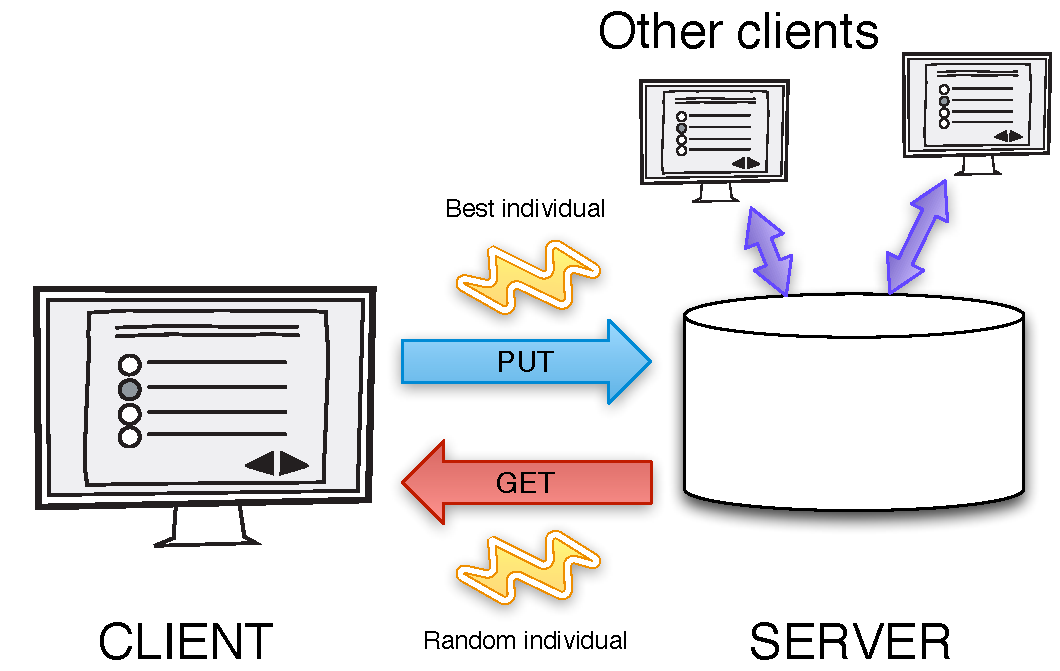
\includegraphics[width=4in]{system.pdf}
\caption{Description of the proposed system. Clients execute a JS EA
  in the browser, which, every 100 generations, sends the best
  individual and receives a random one from the server.}
\label{fig:system}
\end{figure}

The researcher only has to change a function, which can be written in
JavaScript or in any other language with cross-compilation to
JavaScript \cite{web:compilersjs} to solve a different
problem. In this case the classical Trap function \cite{Ackley1987} has been
used as well as the Rastrigin's floating-point optimization
problem. JavaScript is a functional language and declaring a different 
function and handing at the creation of the algorithm object, called
{\tt Classic}, is the only change needed to work with a different
problem. Let us see how this system addresses the different challenges
outlined in the State of the Art (Section \ref{sec:soa}):
\begin{itemize}
\item {\em Scalability} is provided via the use of a lightweight and
  high-performance, single-threaded, server based in Node.js and
  Express.js. Although this single server is a bottleneck since it
  will eventually saturate, the fact that it runs as a non-blocking single thread
  allows the service of many requests. In fact, a limit in the
  number of simultaneous requests will be reached, but so far it has
  not been found, unlike what we found in our previous systems, DCoR,
  \cite{gecco07:workshop:dcor}, which had a low scalability. 
\item The system is {\em heterogeneous} since it does not need any
  performance, operating system, or even browser requirement as long
  as JavaScript is enabled: anyone
  visiting the page, even from mobile devices, can load the algorithm.
  In case the browser does not support HTML5 Web workers (e.g., 
  Windows Phone or some version of Android) or their use
  has been disabled, a basic version of {\sf NodIO} can also be used.
\item {\em Fault tolerance} is always an issue, and in this case, the
  single point of failure would be the server: the system, as such,
  would break down if the server fails. However, the individual
  islands in every browser would continue running, and having access
  to just one of them would allow the local algorithm to proceed. In
  fact, the island does not need the server to run: it runs locally if
  needed, with the only exception that it is obviously unable to
  communicate with the rest of the islands.
\item {\em Adaptiveness} is achieved simply through the autonomous
  operation of every individual island without any synchronization
  mechanism. The islands in the system are, in fact, unaware of each
  other, communicating only through the server. This architecture 
  has been tested in other high demand systems with success, but 
  in the case of {\sf NodIO}, additional experiments are needed to asses 
  the scalability of the communication system. % (Paloma) Is it ok if we talk about scalability when we were talking about adaptiveness? Scalability was also described in the first point.
  %(Mario) Scalability of the communication system in particular?
\item Since the algorithm runs in the browser, {\em safety} is
  achieved through its sandbox mechanisms. The user is thus assured
  that there is no unsafe access either to their local files or even
  to more resources than the browser should be allotted.
\item Running the algorithm is just a matter of loading the page,
  which makes the operation totally {\em anonymous}. For the same
  reason, {\em ease of use} is optimal, being as easy as simply
  clicking on an URL, available to anyone with access to a browser.
\item {\em Reasonable performance} is not ensured. In fact, we should
  make sure that there is a reasonable amount of clients over which
  the performance achieved is better than what you would obtain in
  your own desktop system. If this is not the case, it is a pointless
  academic exercise.
\end{itemize}

There are many different ways to validate a framework that intends to
address these challenges. Some of them are included by design: it is
anonymous, since no accounts are needed to participate in the
experiment, it is safe for the user, since we are using the browser
black box, and it is also heterogeneous. We have designed the
experiments so that they show adaptability to different types of
experiments and clients, scalability with the number of clients and
the problem size, and measured performance by comparing it with
a baseline configuration, with which, as indicated above, is
compatible and can be used in a complementary way. Fault tolerance
will be experimented by dropping the server and checking the continuity
of the experiments. 

All these points will be established in the next two sections,
starting with the baseline, single worker system next. 

%---------------------------------------------------------------
\section{Baseline Experiment and obtained results} %Cambié el nombre
\label{sec:experiments}

\begin{figure}[!t]
\centering
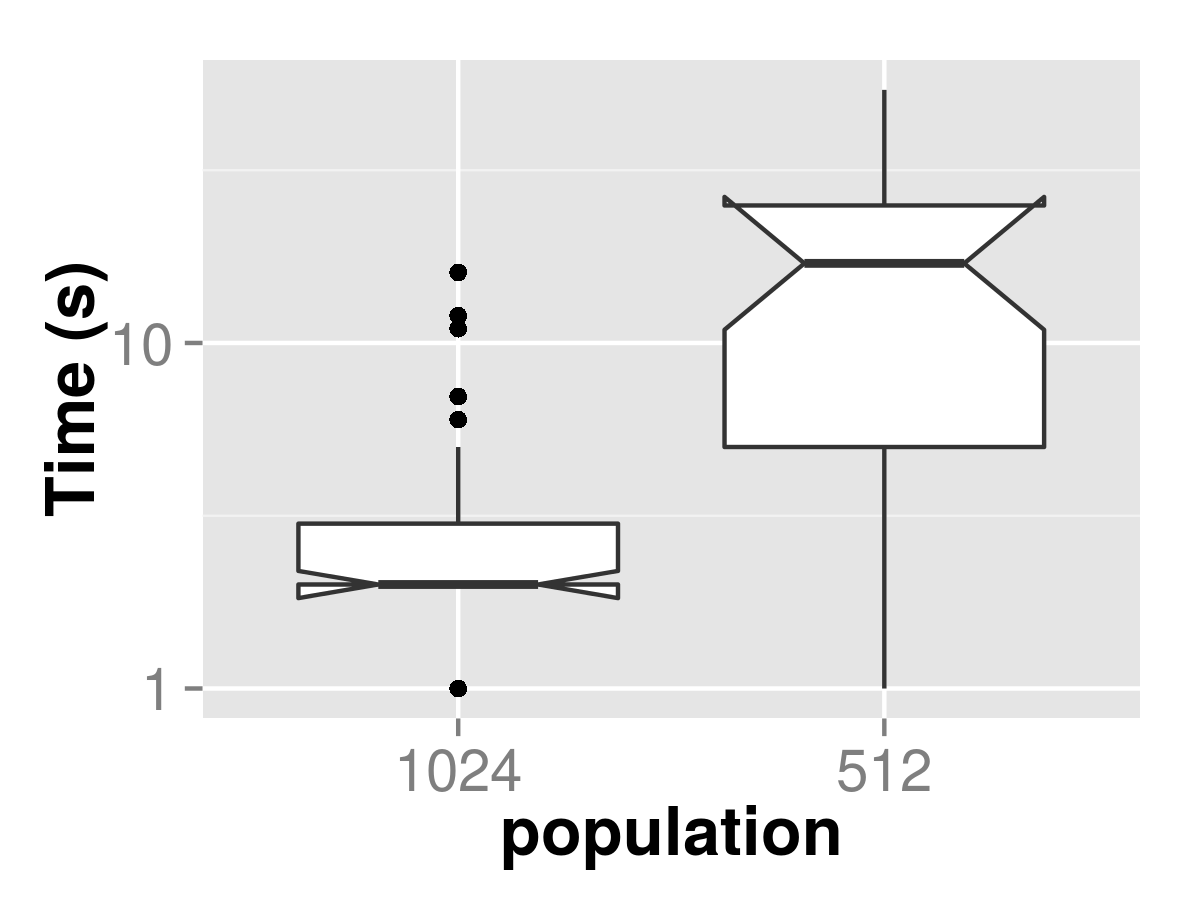
\includegraphics[width=12cm]{baseline-times.png}
\caption{Comparison of times to solution (labeled as {\bf times}) for the baseline system, using a {\tt
    Node.js} client, for different population sizes. Only
runs in which solution has been found are used for this graph.}
% Plotted with: ~/Code/splash-volunteer/data/plot-baseline.R
\label{fig:baseline}
\end{figure}
First, we establish the baseline performance by running the
evolutionary algorithm in a desktop client written using {\sf NodEO}
\cite{nodeo2014}, the basic JavaScript library we have used as base to
build {\sf NodIO}, the framework. This experiment tries to 
find the solution to the 40-trap function with parameters $l=4, a=1,
b=2, z=3$ and a population size equal to 512. The algorithm in a
single island was run until the solution (a string with all
ones) was found or five million evaluations had been performed. It
took around a minute, on average, that is $68.9694$ seconds, to
perform the fifty runs. In this experiment only 33, that is, 66\% were
successful. The experiments were repeated for population $p=1024$,
with a success rate upgraded to 100\% and an {\em average} duration of $3.46$
seconds. Results for these two experiments
are shown in Figure \ref{fig:baseline}. The baseline hardware system has these
characteristics: 
\begin{verbatim}
Linux penny 3.13.0-34-generic #60-Ubuntu SMP Wed Aug 13 15:45:27 UTC
2014 x86_64 x86_64 x86_64 GNU/Linux
\end{verbatim}
with an 8-core {\tt Intel(R) Core(TM) i7-4770 CPU @ 3.40GHz}.

These two experiments establish a baseline result and show that
the time to success depends on the population size, with a bigger population
contributing to have more diversity and thus speeding up the solution \cite{DBLP:conf/lion/LaredoDFGB13}. The volunteer computing
experiments that we will describe next do not and can not have the
same conditions, but
the baseline is that if they eventually take longer than a basic
desktop, their interest will be purely academic. We will try and
prove next that that target performance can be achieved by carrying
out several experiments in different conditions. Second, they also act
as a basic performance test for the server, and also prove that the
basic server can be used for many kinds of different setups, as long
as they follow the REST protocol to deposit and obtain individuals
from the pool. It is obvious that, in this case, the server is not
really needed, since there is a single client and no interaction
between them, but there is a cost in sending and obtaining chromosomes
from the server so it is included for the sake of fairer comparison.

\subsection{Volunteer evolutionary computation: first experiments and results}

Initial experiments were set up using the OpenShift
PaaS, which provides a free tier within which this 
experiment could be performed. That way, and as required, the hardware
and cloud cost for this experiment were zero. Experiments were
announced through a post in Twitter and other social networks, and
results were published here \cite{DBLP:conf/gecco/GuervosG15}. For the
purpose of this paper, we repeated the announcement several times
through the months of April and then by the beginning of August. All
in all, we have the set of runs with the characteristics shown in
Table \ref{tab:runs}. In general, every experiment took several
days. No particular care was taken about the time of the announcement
or the particular wording. Every {\em experiment} consisted in running
until the solution of the 40-trap problem was found. When the correct
solution was sent to the server, the counter was updated and the pool
of solutions reset to the void set. There was no special intention to wait
until all clients had finished, thus it might happen that, in fact,
the islands running in the browser {\em spill} from one experiment to
the next. However, previous experiments have proven that the influence
of these islands in the next experiment is indeed negligible.
%
\begin{table*}
\caption{Characteristics of the volunteer computing initial runs. \label{tab:runs}}
\begin{center}
\begin{tabular}{l|rr}
\hline
Date & \# experiments & Different IPs \\
\hline
April 4th 4/4 & 57 & 191 \\
April 24th 4/24 &  231 & 559 \\
July 31th 7/31 & 97 & 179 \\
\hline
\end{tabular}
\end{center}
\end{table*}
%
\begin{table*}
\caption{Summary of time per run, number of IPs and number of {\tt
    PUT}s per IP in the initial runs. \label{tab:summary:os}}
\begin{center}
\begin{tabular}{l|ccccccc}
\hline
Date & Median \#IPs & Max \#IPs & Median time (s) & Median \#{\tt
  PUT}s & $<$ 69s & $<$ 3.46s & Inter-experiment correlation\\
\hline
4/4 & 5 & 16 & 2040 & 18 & 14.29\% & 5.36\% & 0.0082 \\
4/24 &  5 & 29 & 732 & 11 & 47.39\% & 3.91\% & 0.0934\\
7/31 & 5 & 14 & 260 & 23 & 27.08\% & 1.04\%  & 0.1741\\
\hline
\end{tabular}
\end{center}
\end{table*}
%
The table shows that every run included more than 50 experiments. The
number of different IPs intervening in them varied from more than one
hundred to more than five hundred in the second experiment.

A summary of the results of each run is also shown in Table
\ref{tab:summary:os}, which shows the median number of Internet Protocol addresses (IPs)
intervening in each experiment,  median time needed
to finish the experiment, median number of HTTP {\tt PUT}s per IP, and
then two columns showing the percentage of experiments that took less
than the two baseline experiments shown in the introduction to this
section. The first striking result is that in all cases, 50\% of the
experiments involved 5 or less IPs. This is consistent with results
previously obtained \cite{DBLP:conf/gecco/GuervosG15} which found 6 to be
the usual number of IPs that participated in an experiment. The
maximum number of different IPs for each experiment is also in the
same range and of the order of 10, which is also consistent with
prior work. The median time has a big range of variation, but 50\% of
the time takes less than several minutes, from around 4 minutes in the
best case to roughly 2/3 of an hour in the worst case. That figure is
not competitive, {\em a priori}, with the baseline experiment, that is
why it is interesting to look at the columns which measure
the percentage of experiments in which the solution was found in less
time than the baseline. It is similar in all three cases, with around
20\% on average for the first baseline experiment, roughly 3\% in the
second case. The comparison is not totally fair: this experiment takes
place in a browser, and in fact most of the time is devoted to
presenting the charts; the server is also not the same since it is run in a
PaaS instead of a high-performance desktop computer, and it is also a
remote server, not a local server as in the baseline experiment. But
even in this case, we were looking for creating a framework that
allowed us to run evolutionary computation experiments {\em faster} than
in our very own computer. And the results indicate that although it will
happen in 1 out of roughly 5 or roughly 20 cases, depending on what baseline
experiment you choose, it will not happen always or even most of
the time. One of the problems is shown in the last column, which
indicates the statistical correlation between the number of IPs
participating in one experiment and the next. In all cases,
correlation is so low as to affirm that there is almost no
relationship between them, that is, computing nodes are not {\em
  staying} after the solution has been found. This is a feature of
this implementation: the user has to actively reload the page to make
the evolutionary algorithm start again. Thus, the user can decide if to continue sharing resources or not.% (Paloma) Feature or disadvantage?
 However, it puts a probably            % (Mario) Feature if you only want to share your CPU a little  
unnecessary upper limit on the time, or number of experiments, that a user
will voluntarily perform.

\begin{figure}[!htb]
\centering
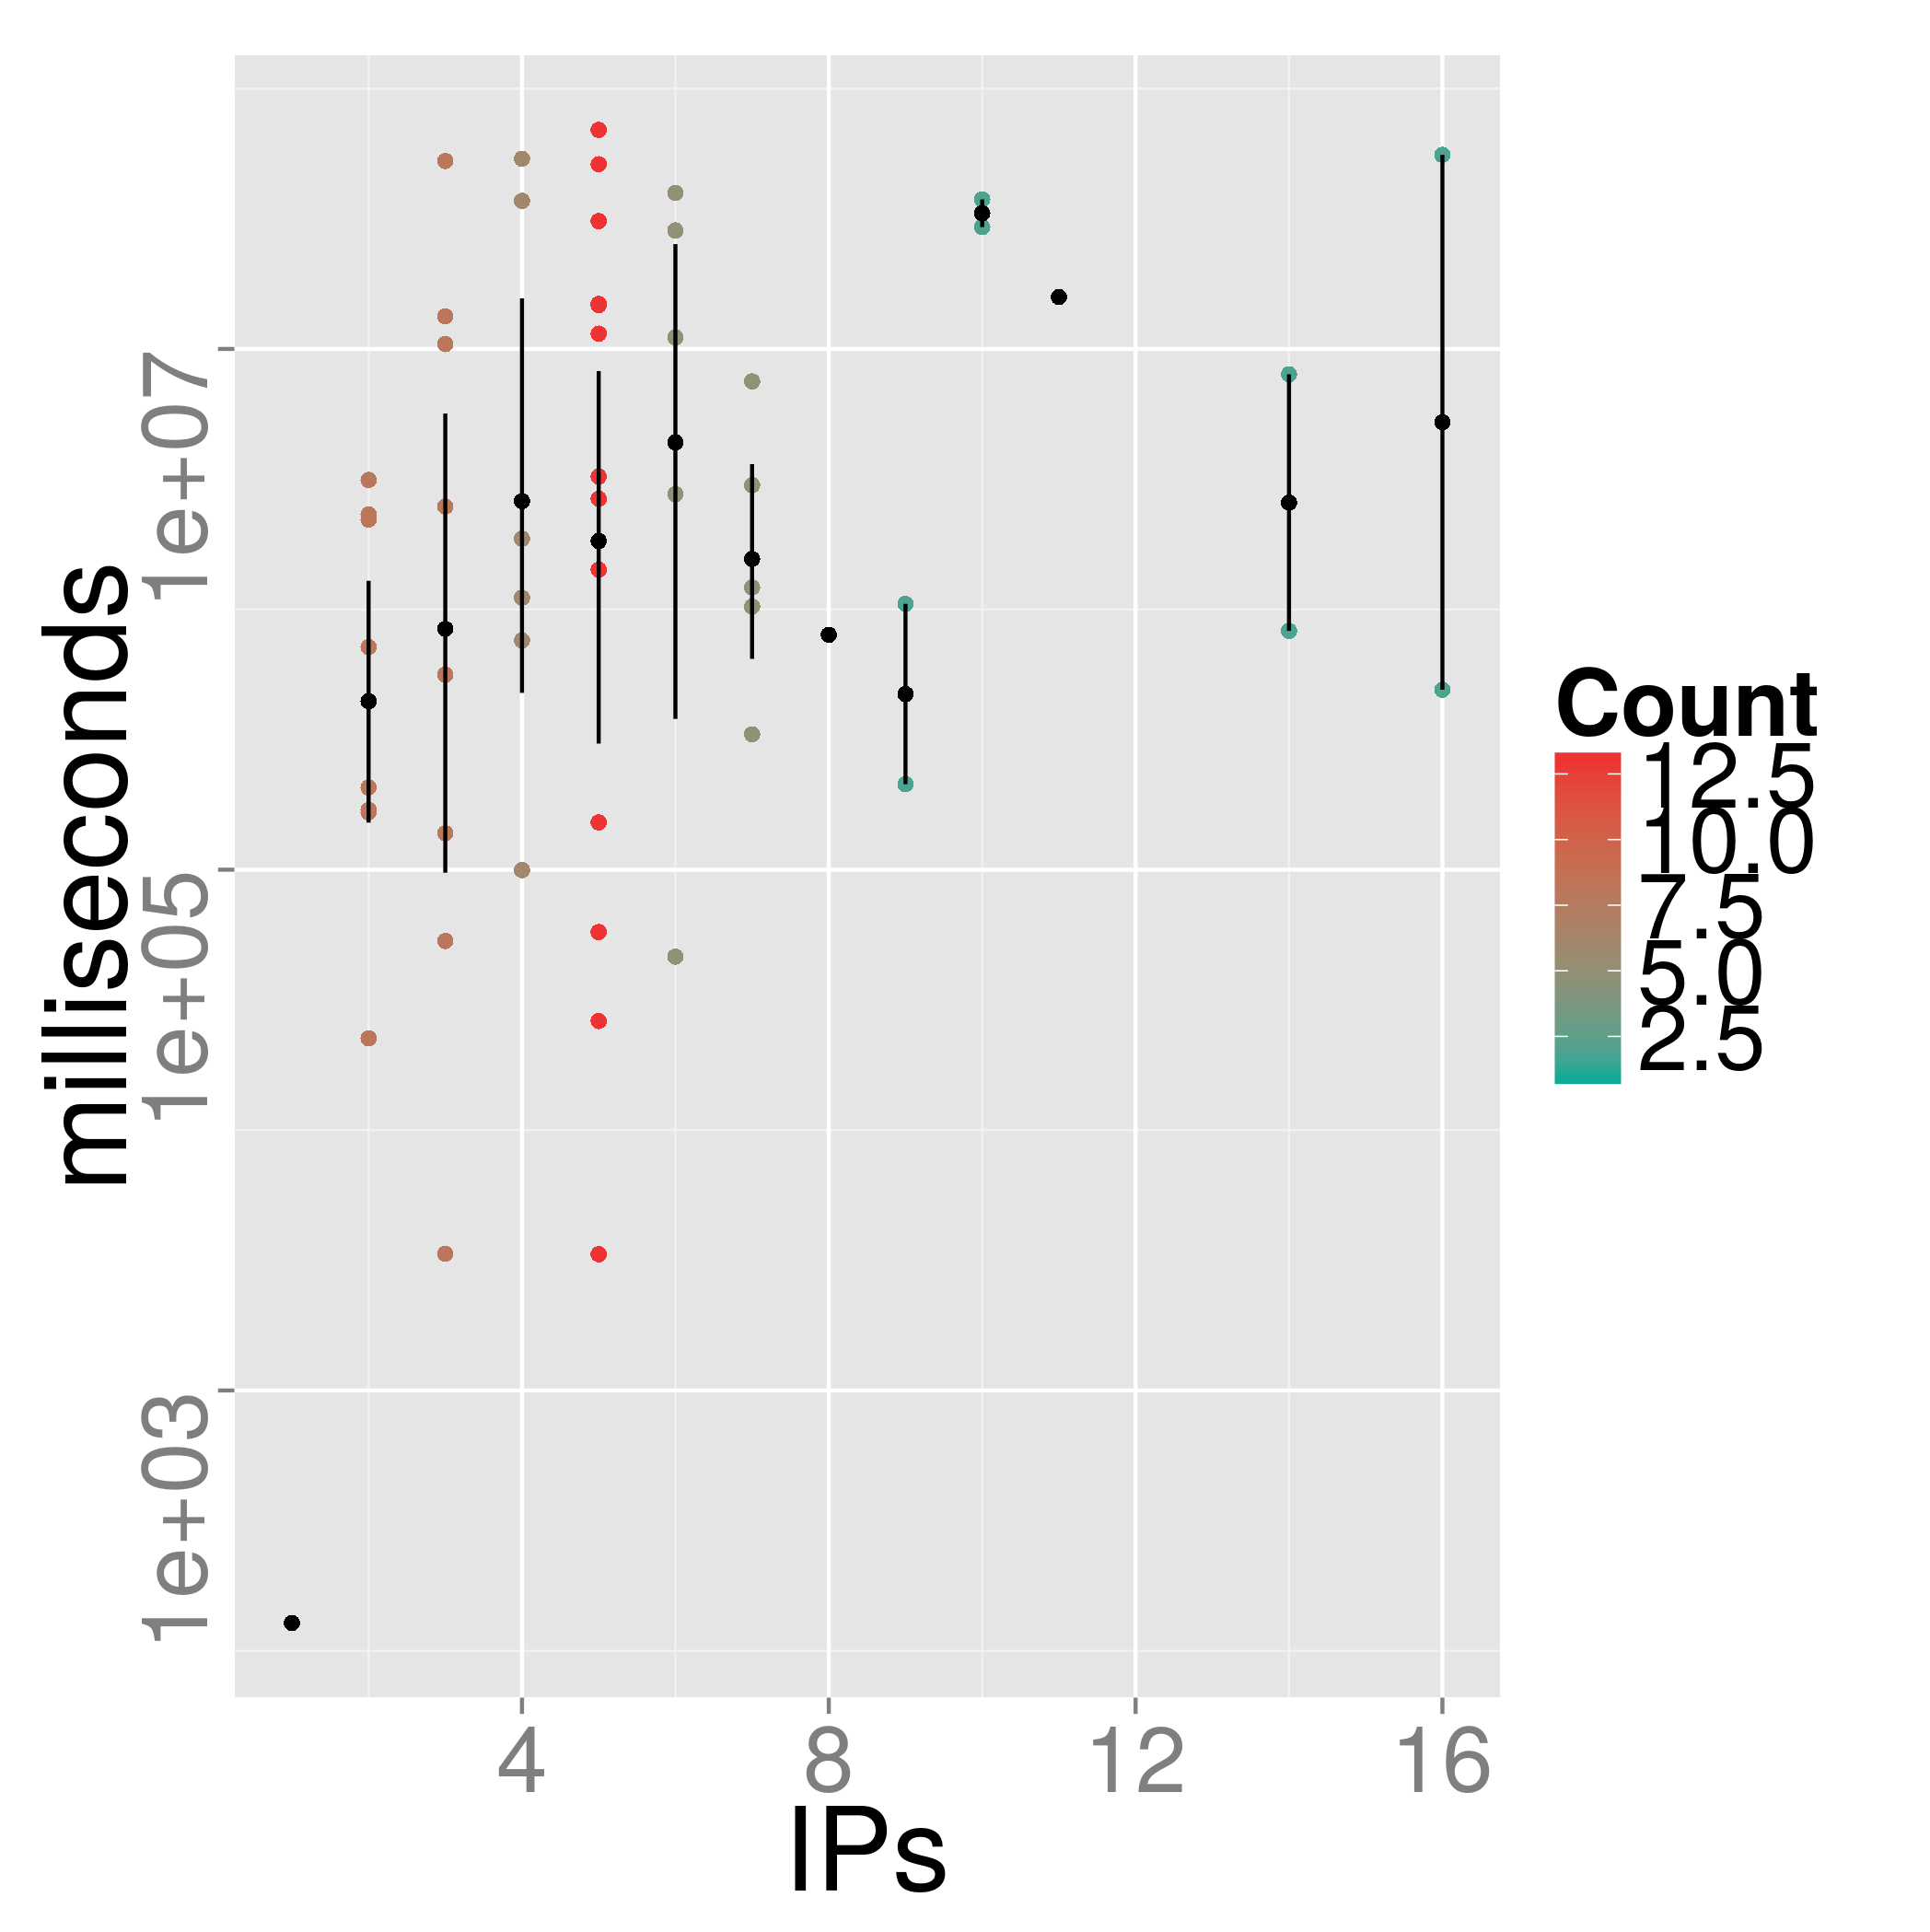
\includegraphics[width=0.32\linewidth]{time-vs-ips-OS-4-4.png}
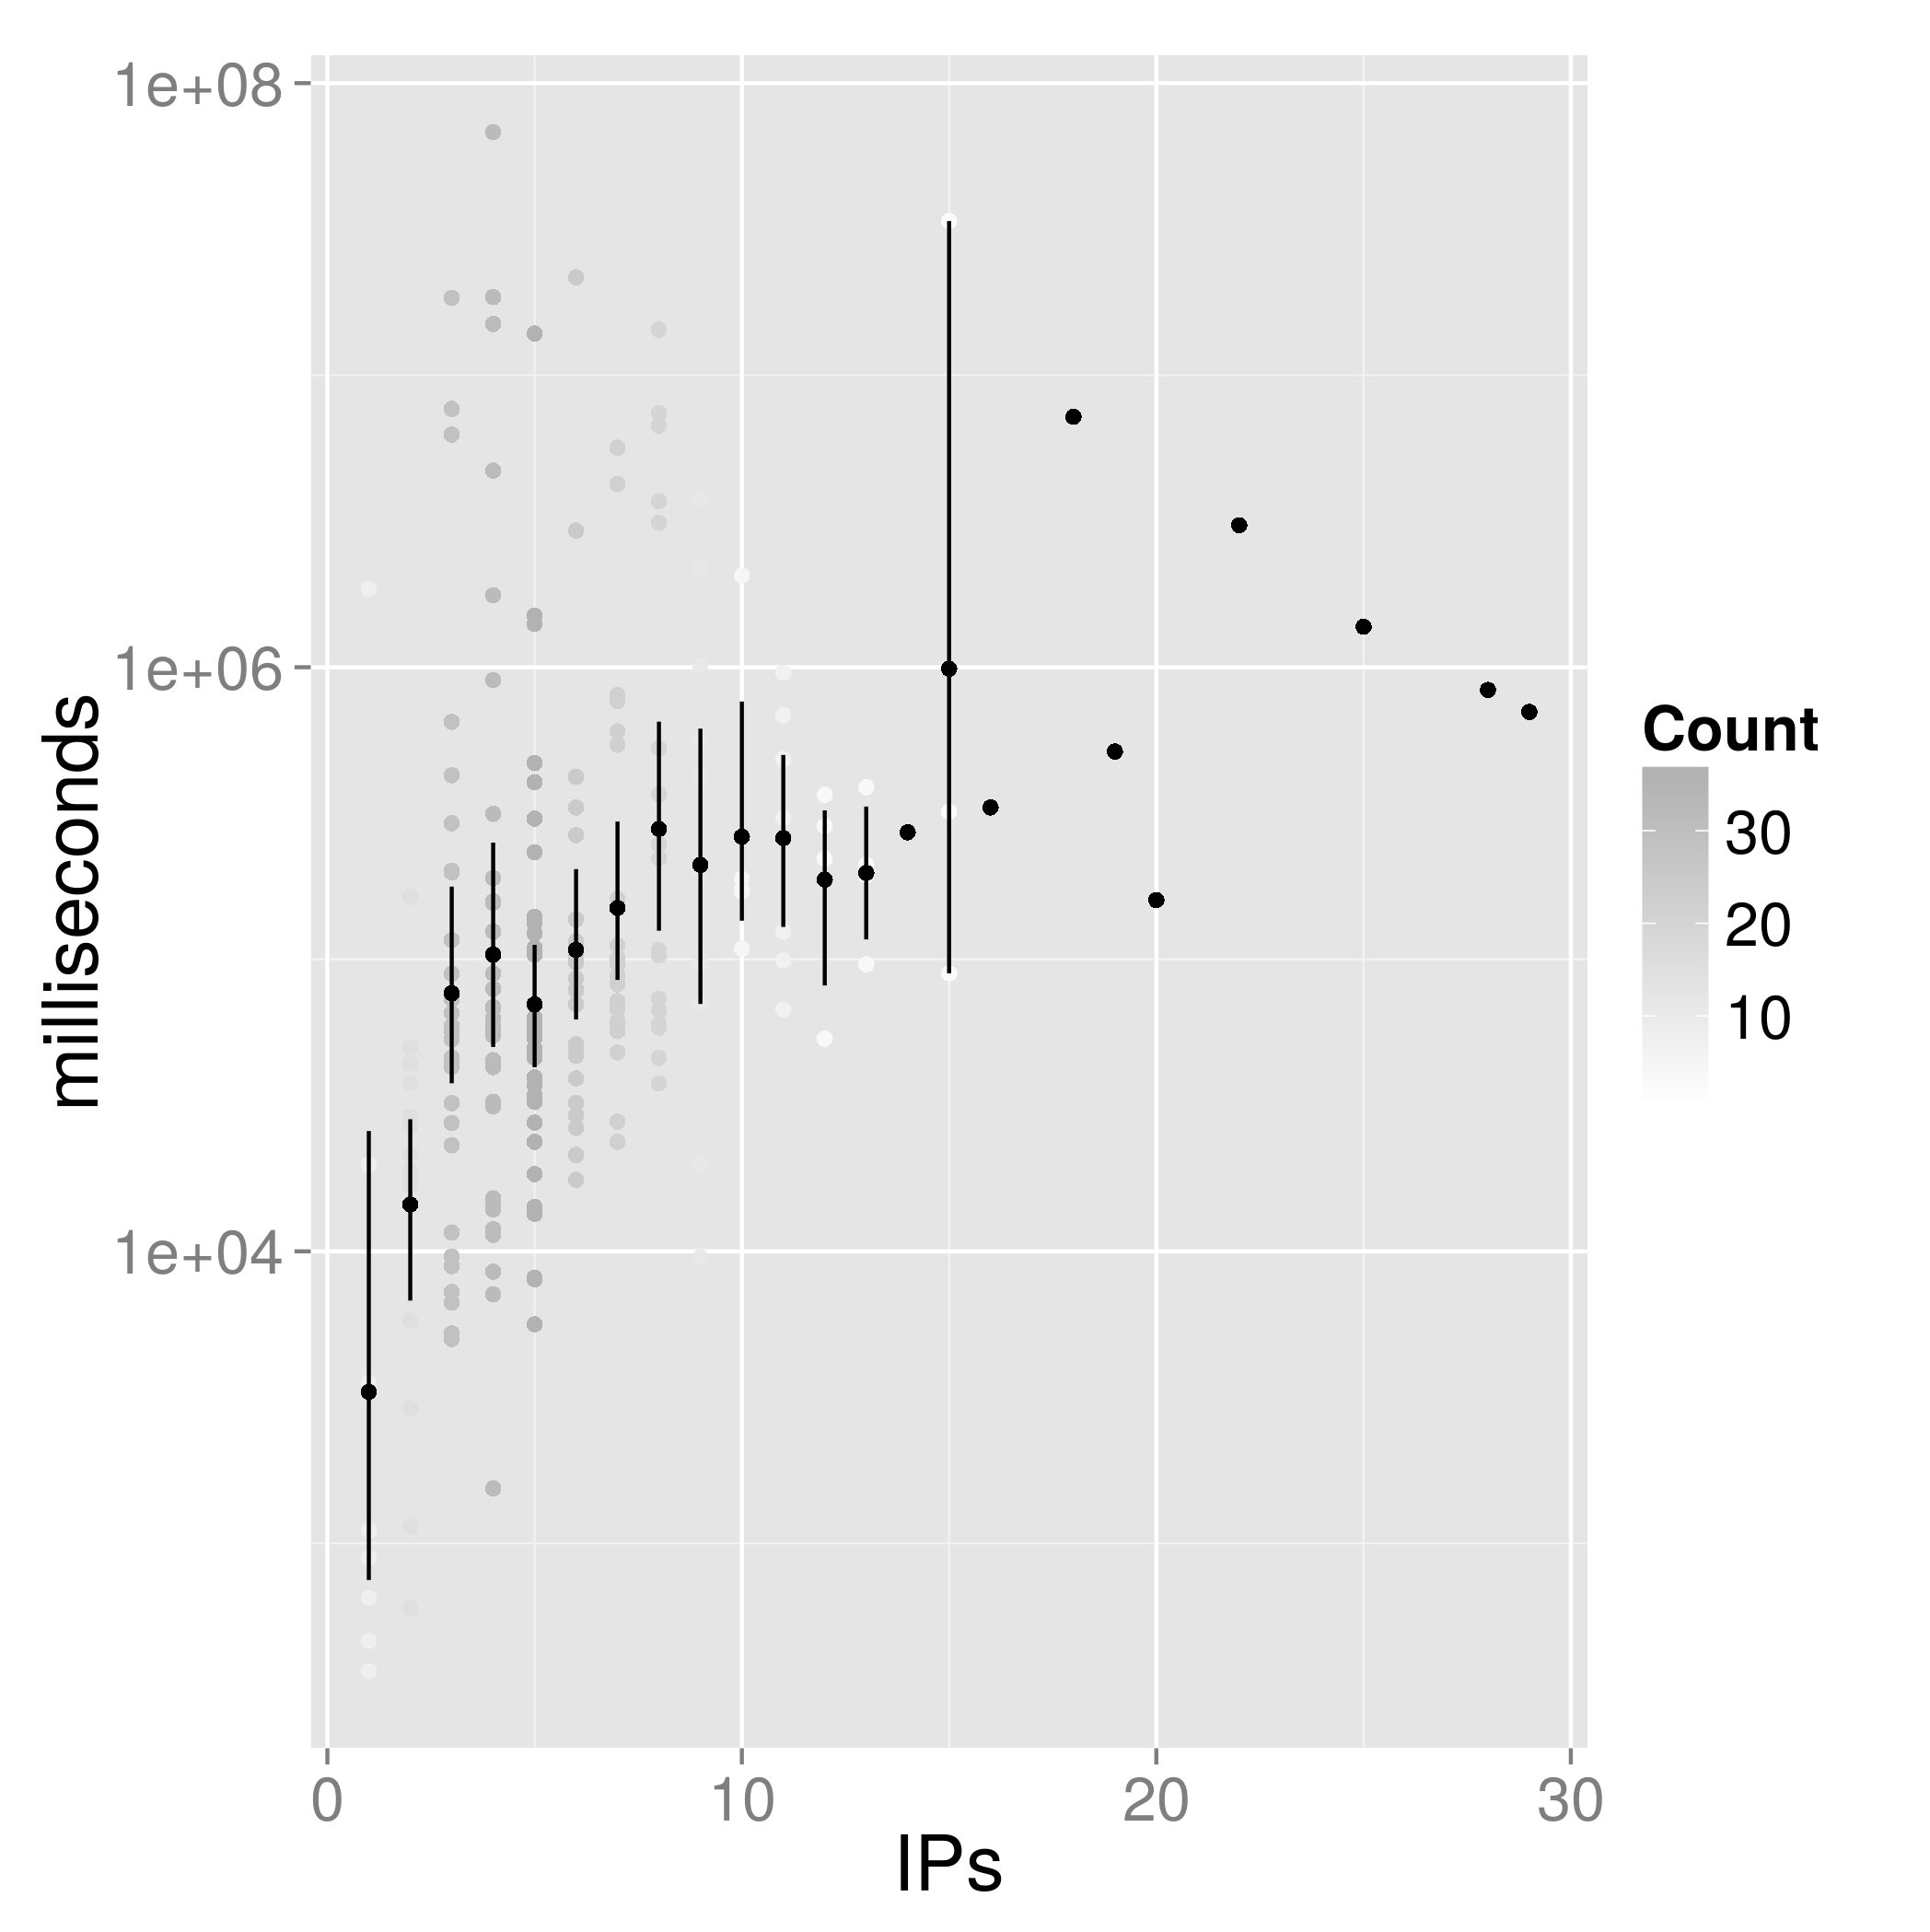
\includegraphics[width=0.32\linewidth]{time-vs-ips-OS-4-24.png}
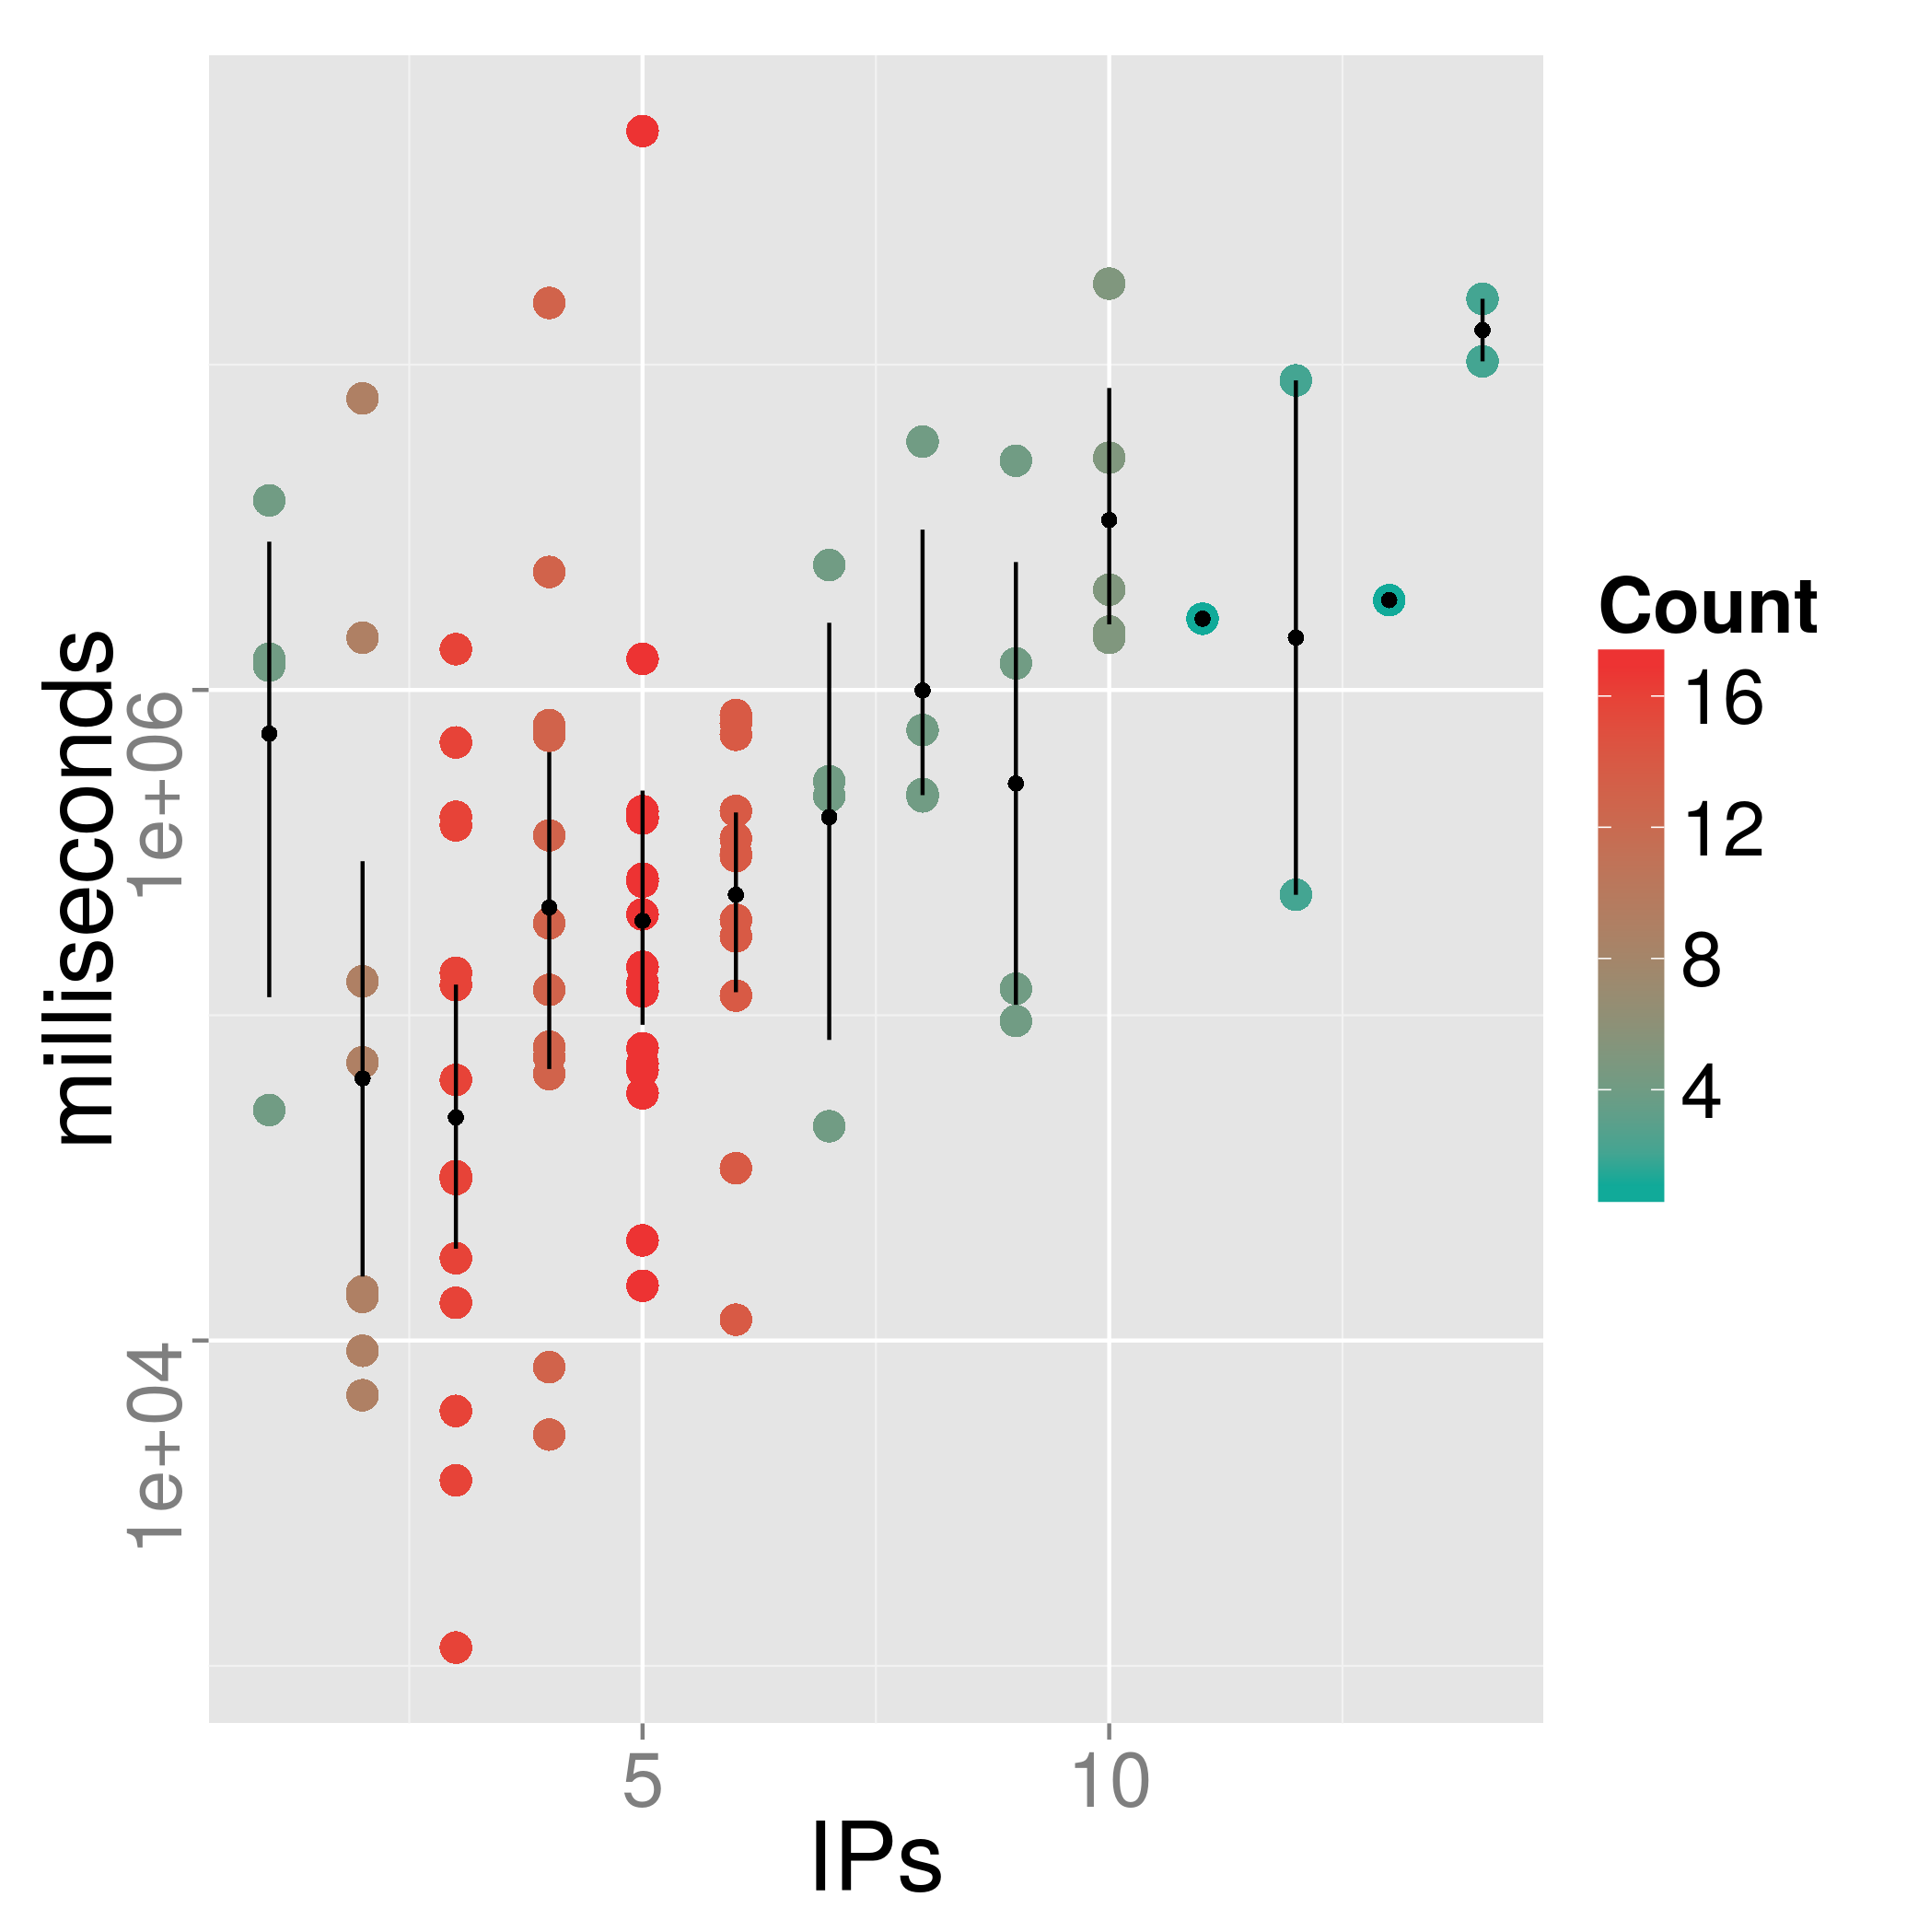
\includegraphics[width=0.32\linewidth]{time-vs-ips-OS-7-31.png}
\caption{Duration of experiments vs. number of different IPs (nodes)
  participating in it, with averages and standard deviation shown as
  red dots; in the case there is a single red dot, there was a single
  experiment in which many computers participated (for instance, 16
  computers in the experiment in the far left or 29 in the middle
  one). 
Shades
of blue indicate how many experiments included that many unique IPs,
so lighter shade for a column of dots indicates that a particular number
of computers happened less frequently, while darker shadow means more frequency. From left to right, experiments 4/4, 4/24 and 7/31.}
\label{fig:duration}
\end{figure}
%
\begin{figure}[!htb]
\centering
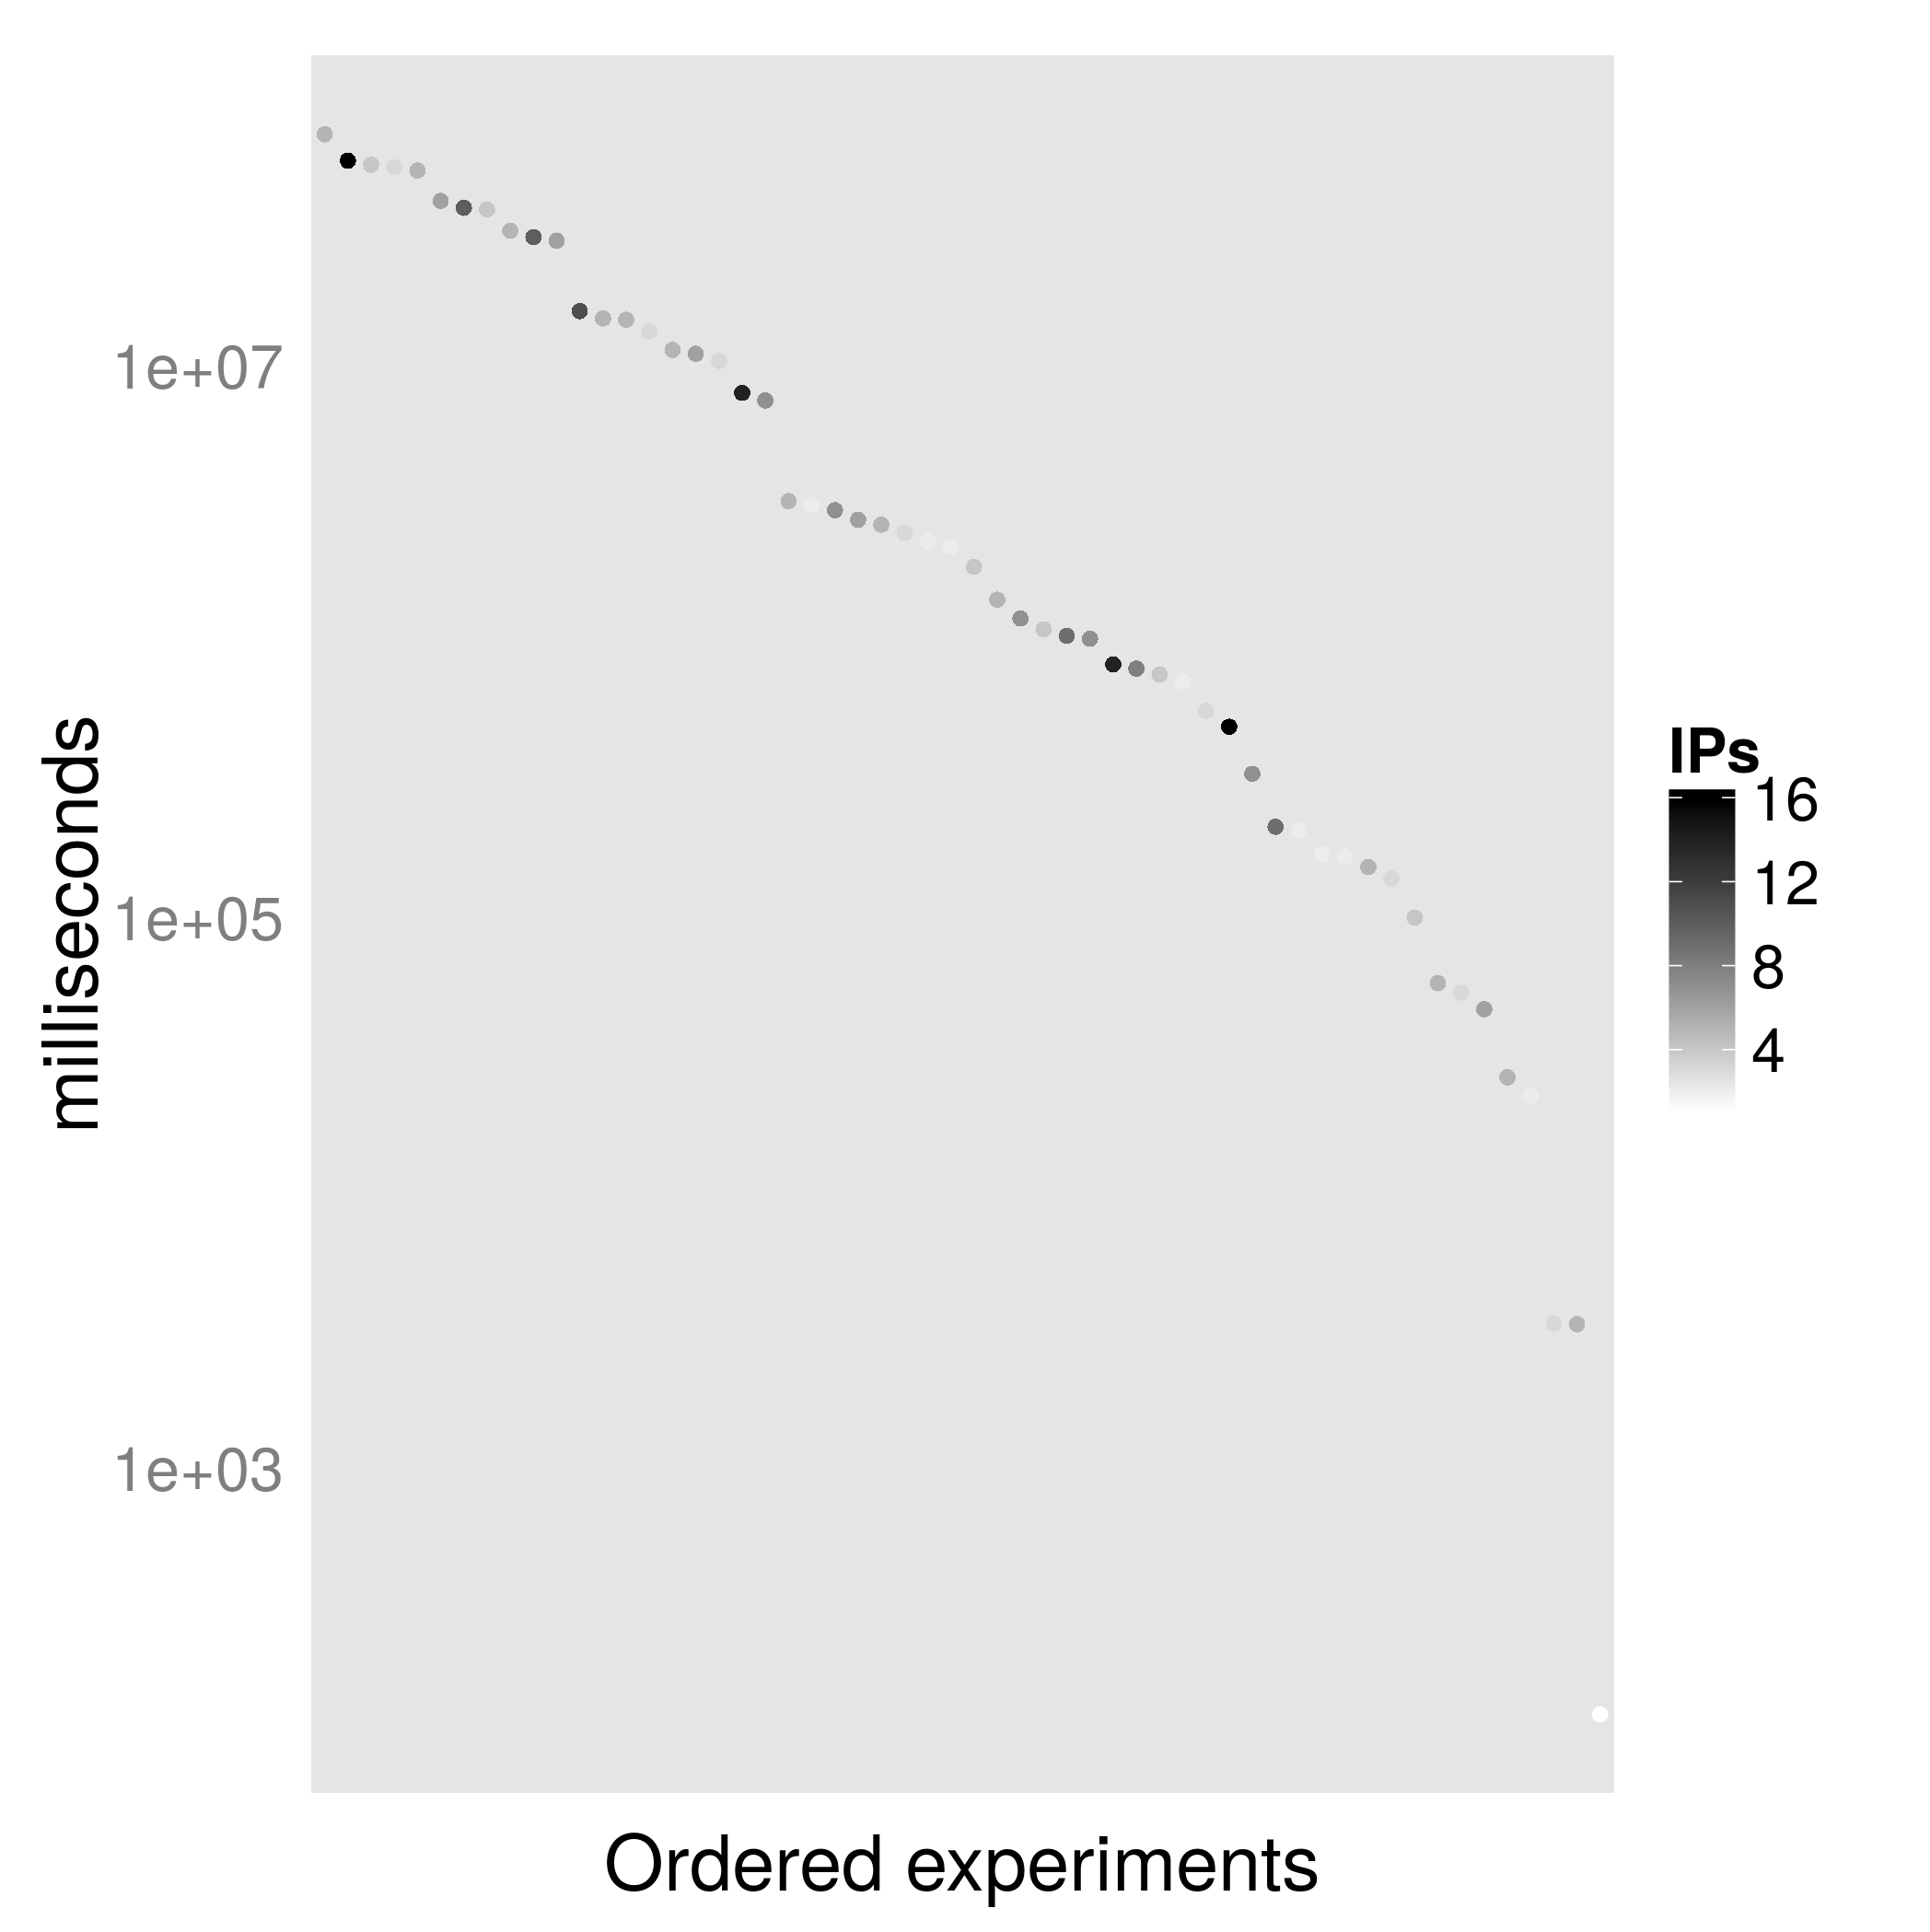
\includegraphics[width=0.32\linewidth]{time-vs-rank-OS-4-4.png}
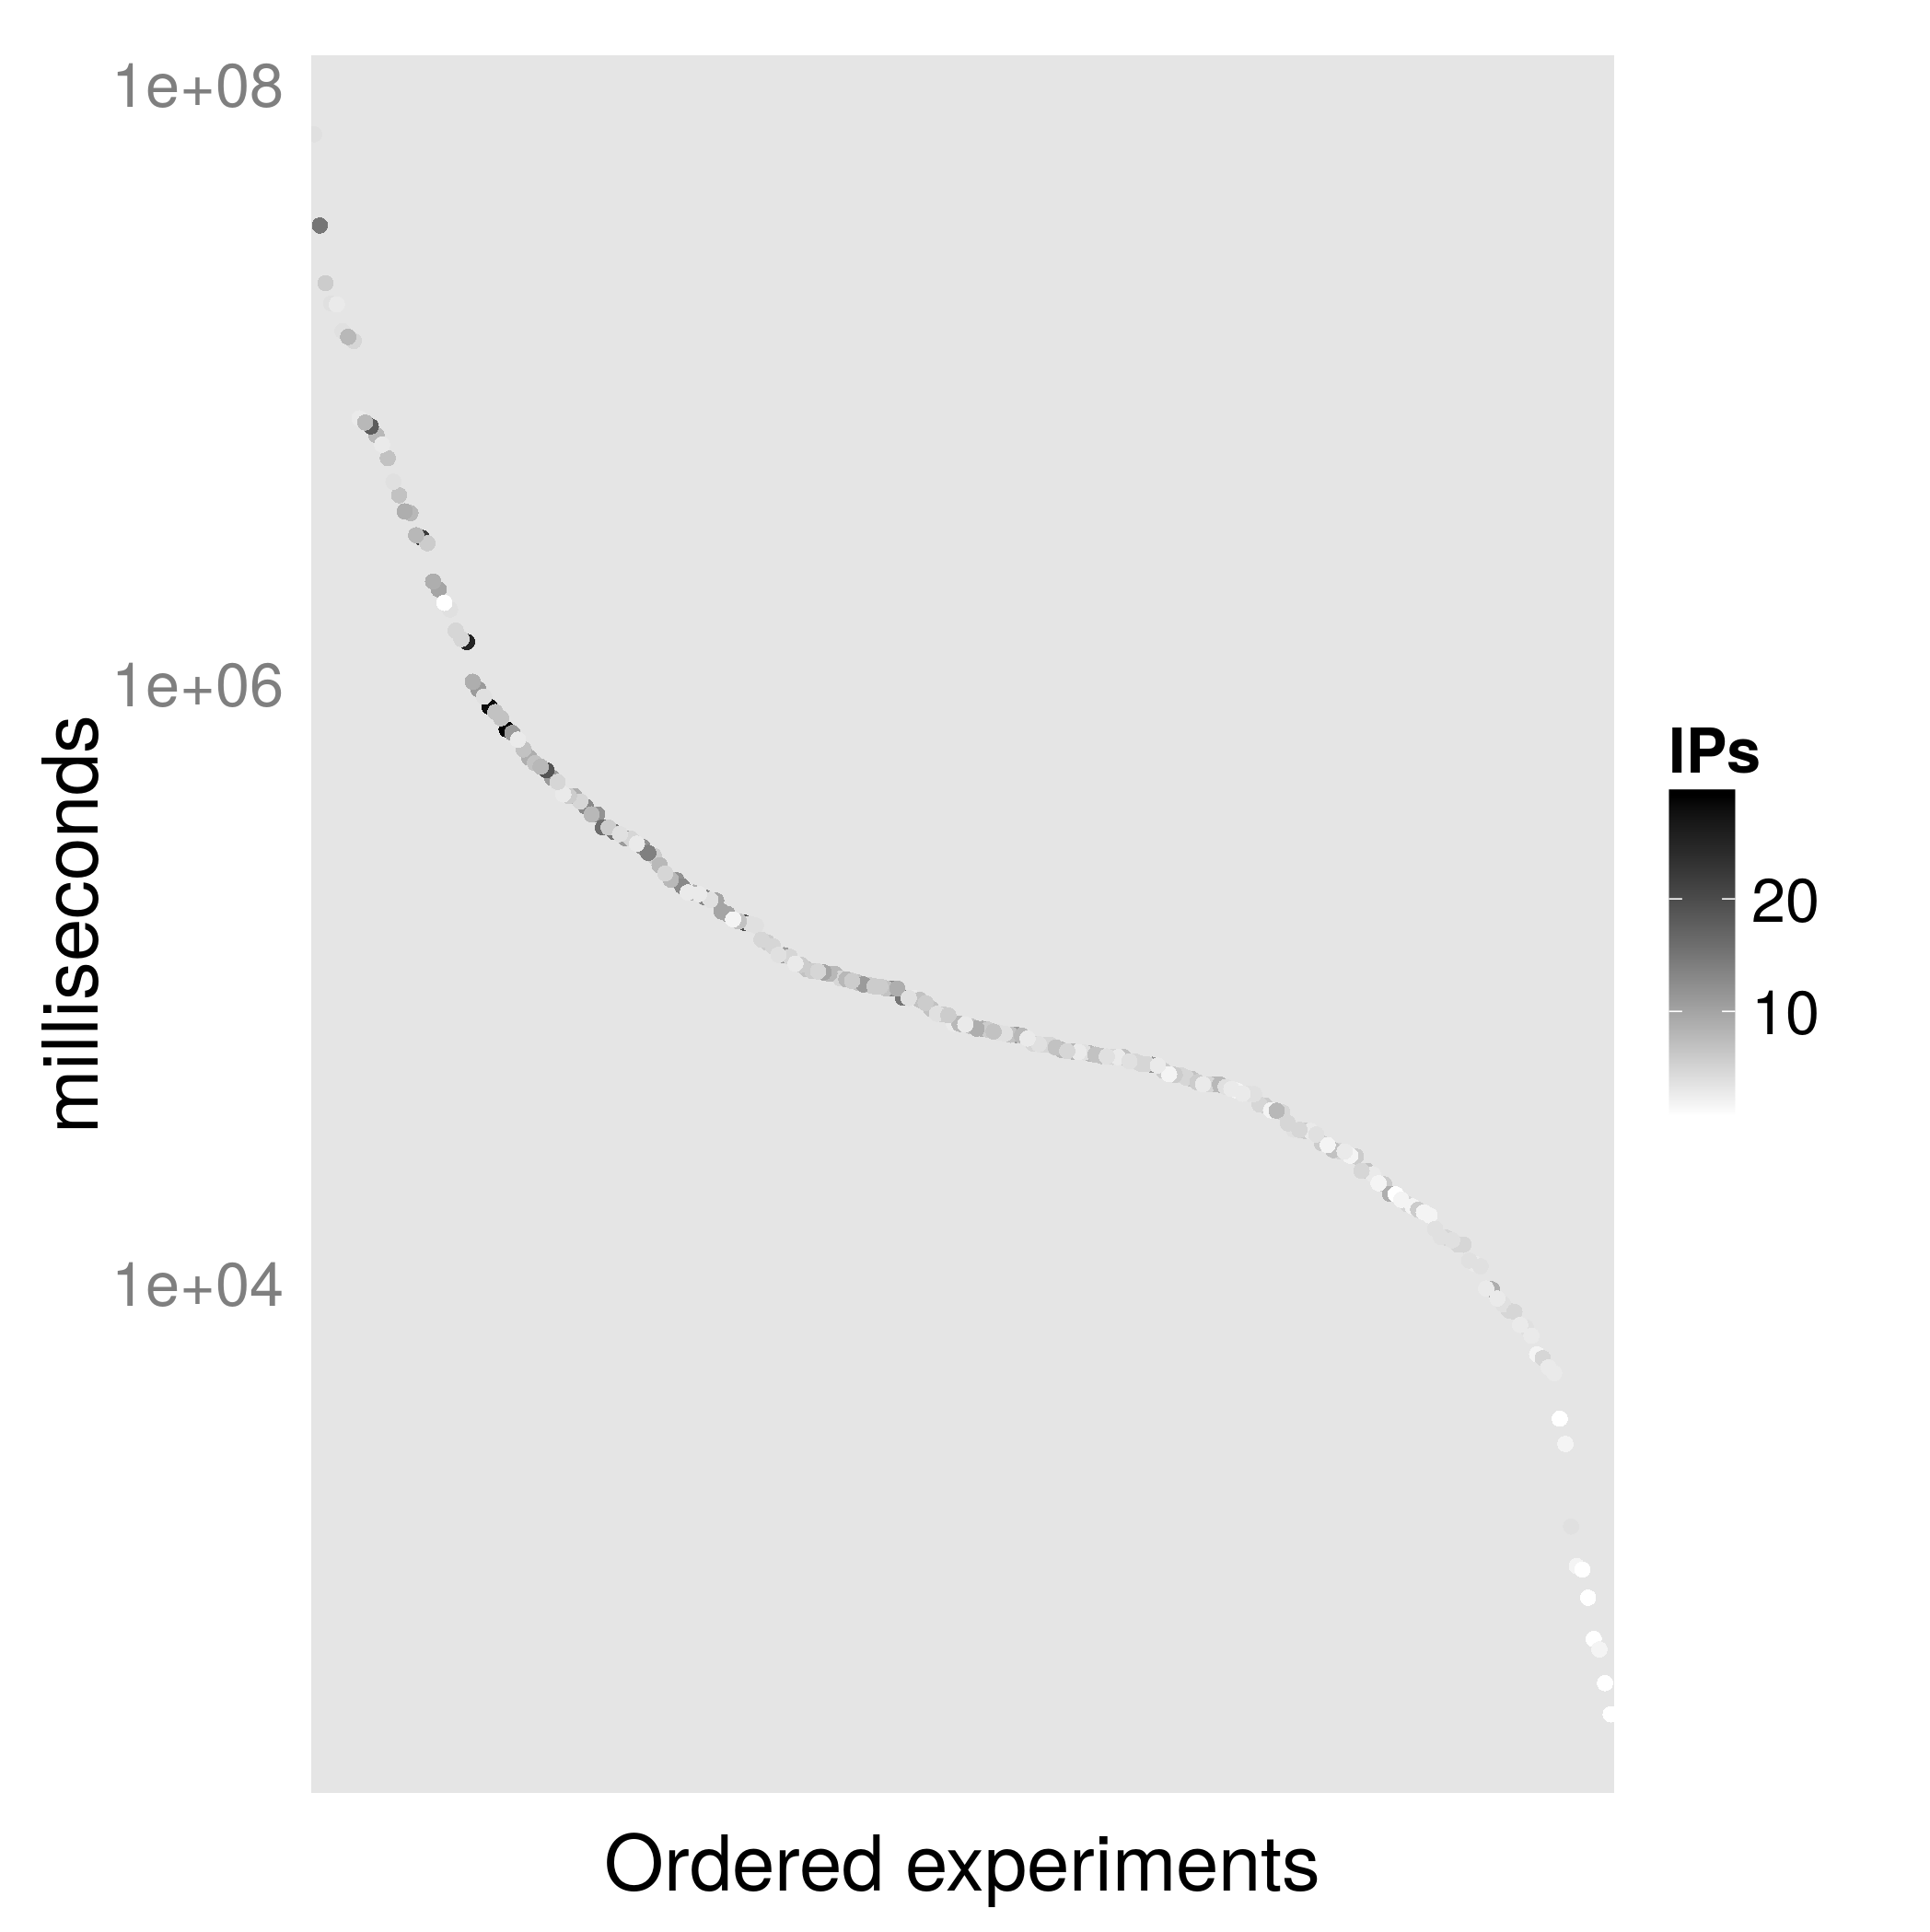
\includegraphics[width=0.32\linewidth]{time-vs-rank-OS-4-24.png}
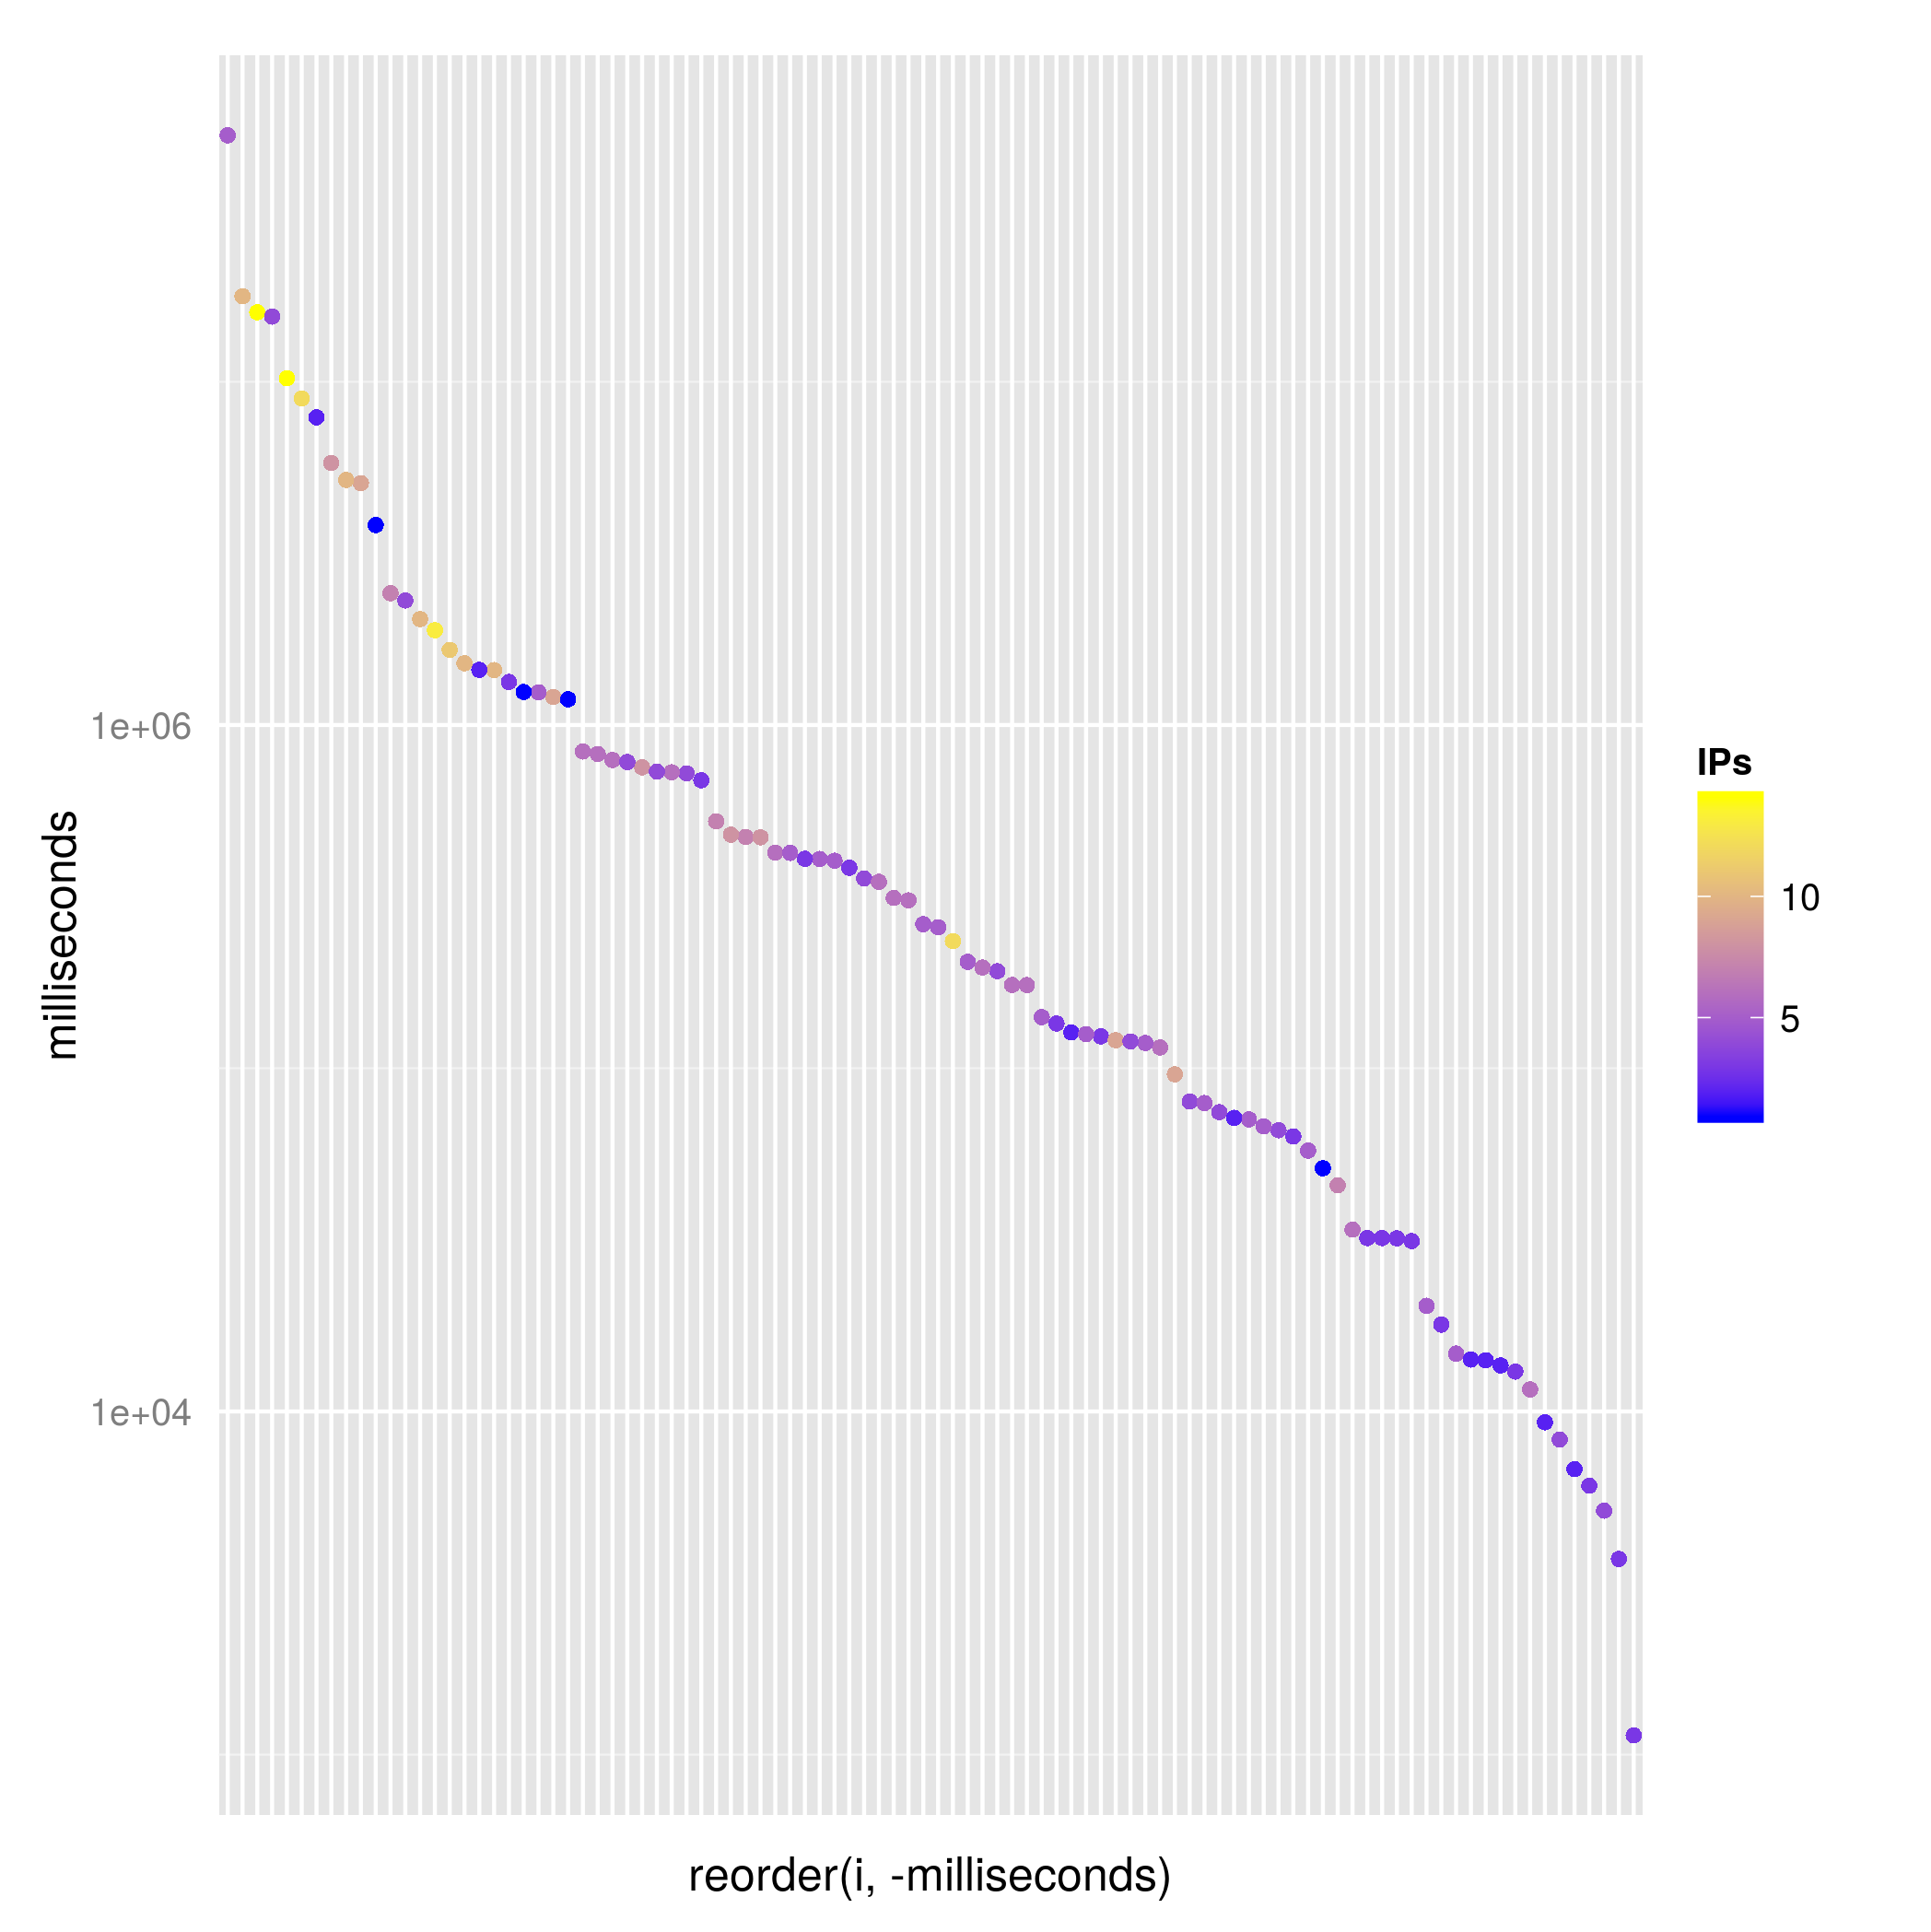
\includegraphics[width=0.32\linewidth]{time-vs-rank-OS-7-31.png}
\caption{Duration of experiments vs. rank, with $y$ axis in a
  logarithmic scale. Dot color is related to the number of IPs
  participating in the experiment. From left to right, experiments
  4/4, 4/24 and 7/31.} 
\label{fig:zipf:os}
\end{figure}
%
We will have to analyze experimental data a bit further to find out why
this happens and also if there are some patterns in the three sets of
experiments. An interesting question to ask, for instance, is if
by adding more computers makes the experiment take less. In fact, as
shown in Figure \ref{fig:duration}, the {\em addition} of more computers does
not seem to contribute to decreasing the time needed to finish the
experiment. However, the cause-effect relationship is not clear at
all. It might be the opposite: since experiments take longer to finish
and might in fact be abandoned with no one contributing for some time,
that increases the probability of someone new joining them. In fact,
with experiments taking a few seconds and due to the way the
experiments are announced, it is quite difficult that several
volunteers join in in such a short period of time, even more if we take
into account that volunteers are not {\em carried over} from previous
experiments. This implies that it would be convenient to use a problem
of a bigger size to check this hypothesis as we have done in the next
experiment. 
%  however, at this point we
% have not found this convenient since there are several other issues
% that have to be solved, as it will be shown next. %Creo que este párrafo
%saldría sobrando ahora que hicmios un experimento más grande

\begin{figure}[!htb]
\centering
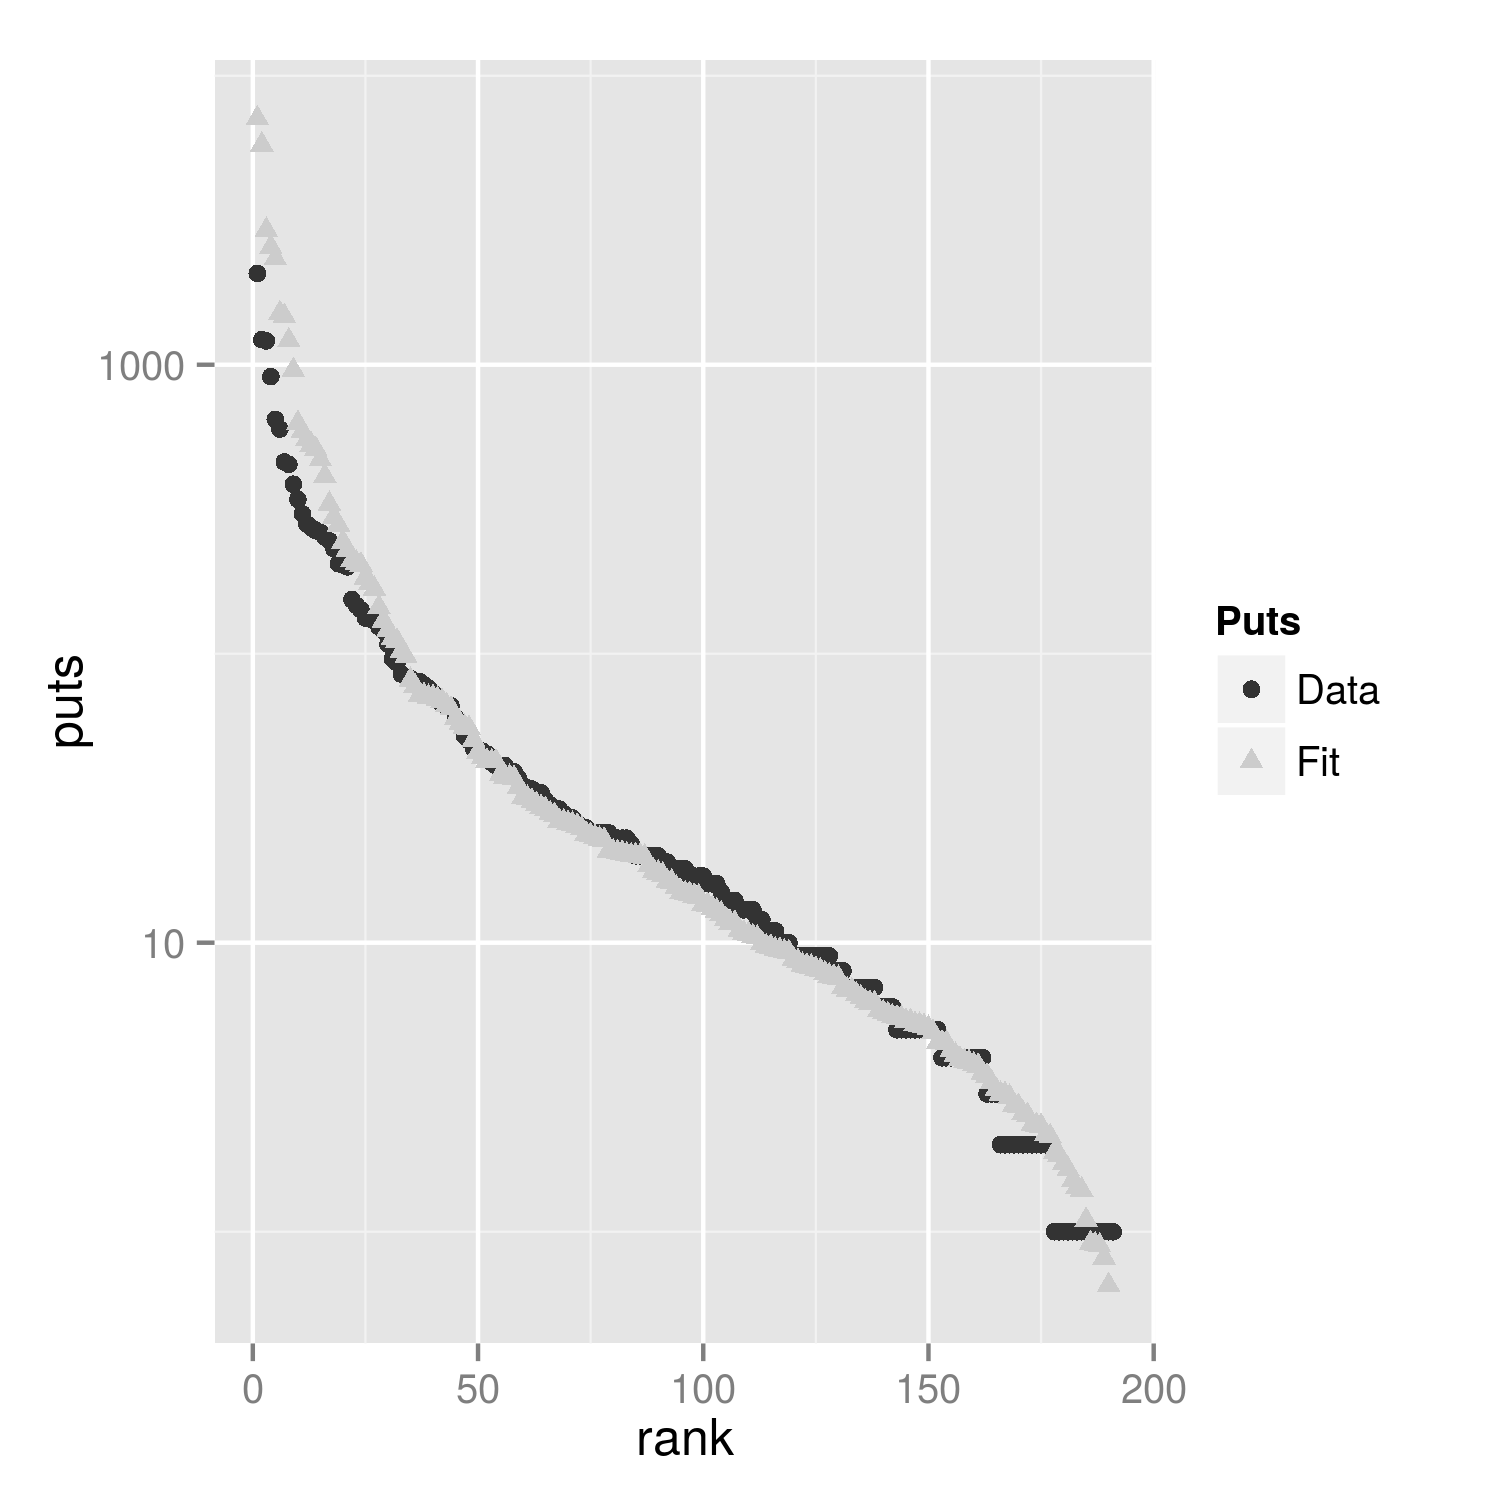
\includegraphics[width=0.32\linewidth]{puts-openshift-4-4.png}
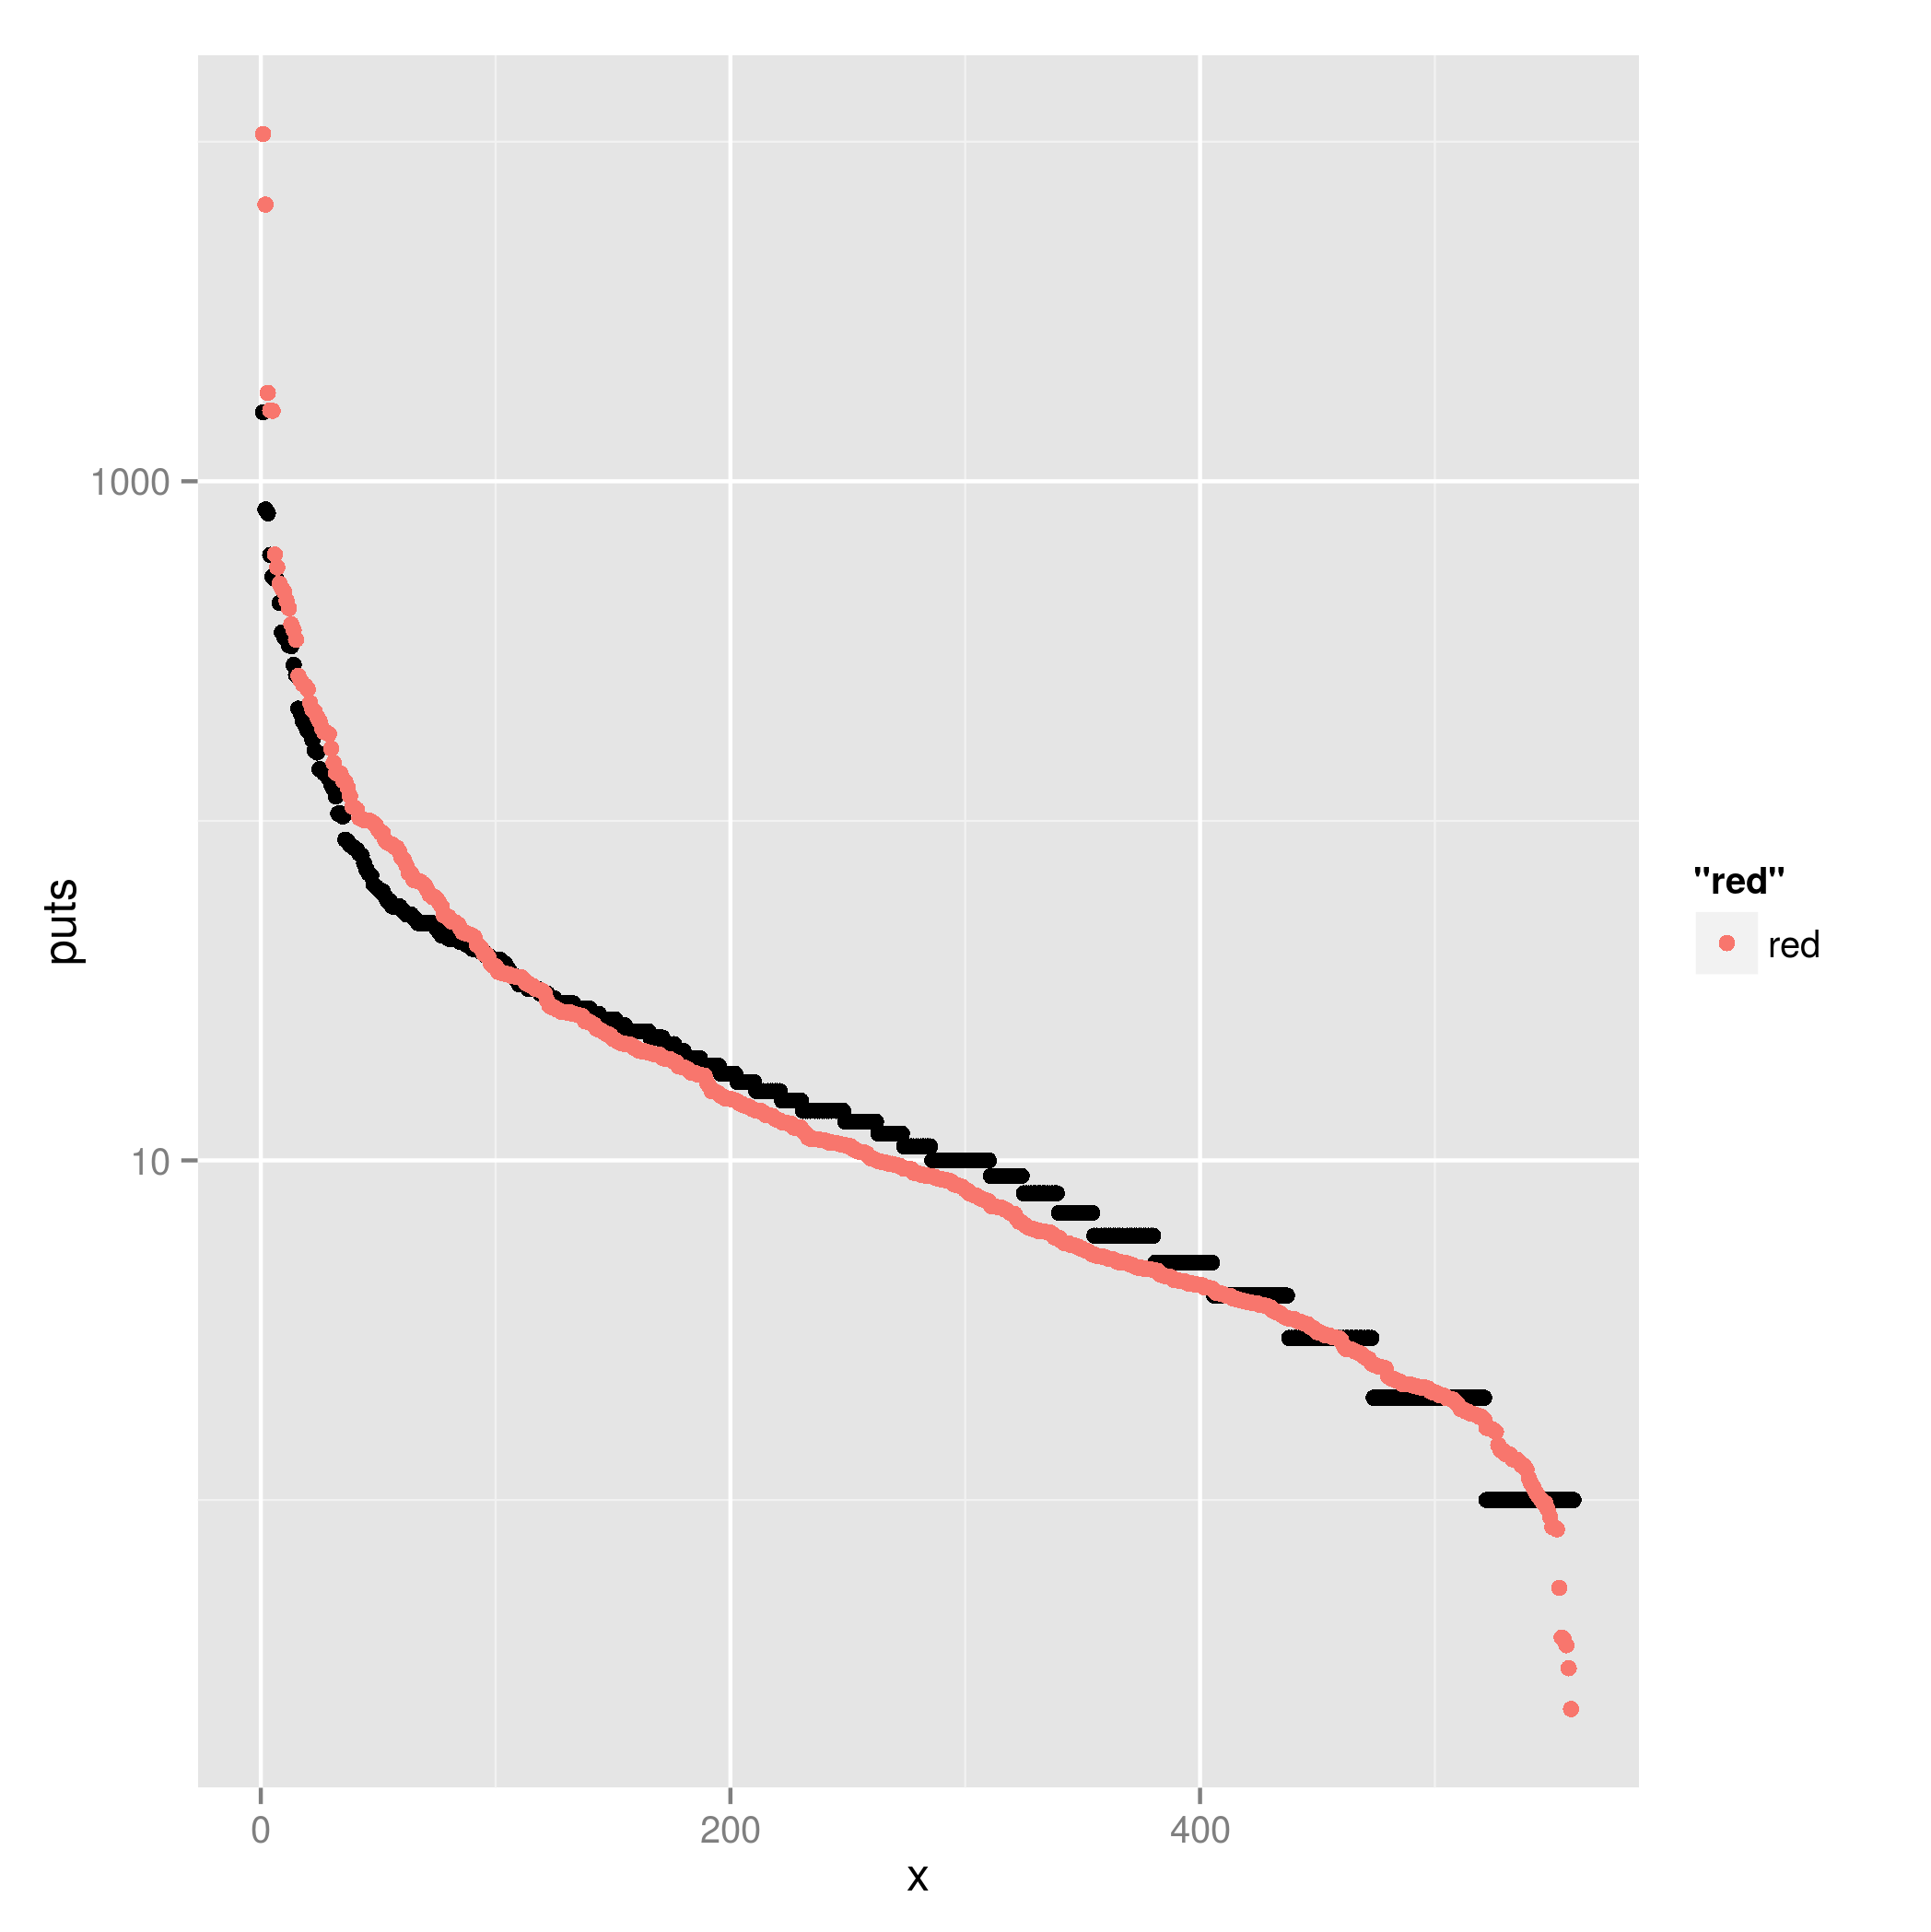
\includegraphics[width=0.32\linewidth]{puts-openshift-4-24.png}
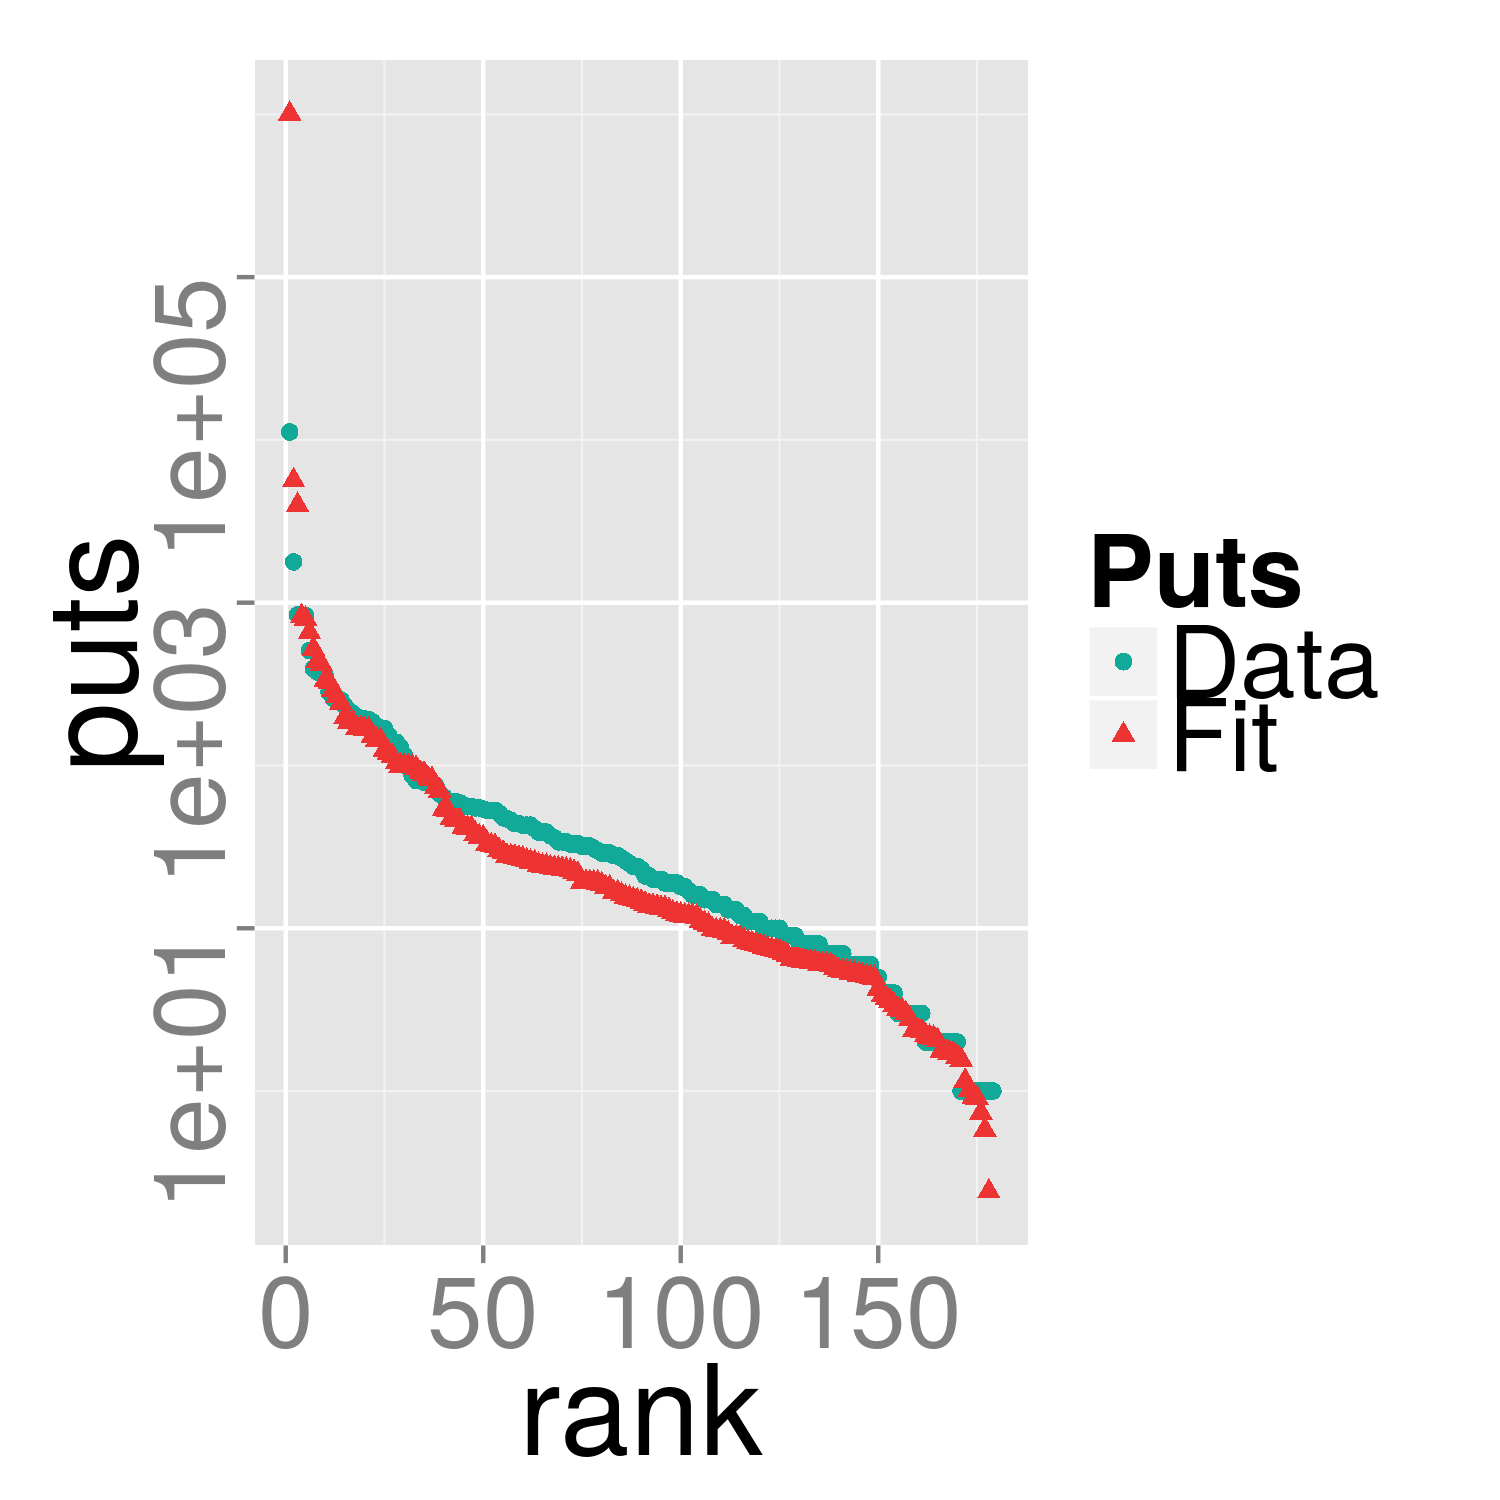
\includegraphics[width=0.32\linewidth]{puts-openshift-7-31.png}
\caption{Number of {\tt PUT}s per unique IP and fit to a Generalized
  Extreme Value distribution (in red). From left to right, experiments
  4/4, 4/24 and 7/31.} 
% Plotted with ../data/plot-zipf-openshift.R
\label{fig:puts:os}
\end{figure}
%
It is also interesting to check the distribution of the experiment
duration, shown in Figure \ref{fig:zipf:os} and which roughly follows
a Zipf's law, with similar distribution along all three runs. The 4/24
run is the most complete and shows a S-shape, which implies an
accumulation of experiments taking similar time and around 100
seconds. The most interesting part is the {\em tail}, which shows how
many experiments took a desirable amount of time, of the order of
10 seconds, and which appears in all three graphs. As it can be seen,
it sharply drops implying there are 
just a few of them, and with diminishing probability as time
decreases. This exponential distribution also appears in the
distribution of HTTP {\tt PUT}s, equivalent to the number of
generations divided by 100, contributed by every user, which is shown
in Figure \ref{fig:puts:os}. These results show a Zipf-like behavior,
so we have fitted it to the Generalized Extreme Value distribution,
with the resulting parameters shown in Table \ref{tab:puts:os}.
%
\begin{table*}
\caption{Summary of fit to Generalized Extreme Value distribution of
  the number of {\tt PUT}s per unique IP. \label{tab:puts:os}}
\begin{center}
\begin{tabular}{l|ccc}
\hline
Date  & Location $\mu$ & Scale $\sigma$ & Shape $\xi$ \\
\hline
4/4 &  8.541 $\pm$ 1.0926  &    12.442 $\pm$ 1.7302 &  1.388 $\pm$
0.1377 \\
4/24 & 6.148 $\pm$ 0.3782 & 7.354 $\pm$ 0.5105 & 1.090 $\pm$  0.0697  \\
7/31 & 11.645 $\pm$ 1.475 & 16.365 $\pm$ 2.201 &  1.265 $\pm$ 0.132   \\
\hline
\end{tabular}
\end{center}
\end{table*}
%
This distribution was originally proposed to fit extreme values
\cite{resnick2013extreme} and contains, as a special case, the inverse
Weibull distribution which was fitted to volunteer computing
frameworks such as SETI@home \cite{javadi2009mining}. We obviously do
not pretend to compare our system in scale or complexity with it, but
to point out that the behavior of volunteer computing nodes follows a
certain pattern, found in SETI@home, and which also appears in our system. This
distribution is governed by three parameters, the usual location $\mu$
which is related to where it has its {\em center} and a scale $\sigma$,
related to the size, but also a third shape $\xi$ parameter that is
related to its skewness, that is, how skewed it is around the central
location. Positive parameters indicate that the distribution {\em
  leans} towards the origin, and negative ones towards the other extreme
value. In this case, Table \ref{tab:puts:os} shows $\xi$ values
greater than one and between one and 1.4, which indicates that the
three experiments share this origin-leaning pattern, with many users
donating a few cycles and just a few donating extreme values. Random
distributions with these parameters have been plotted in red in
Figure \ref{fig:puts:os}, indicating that the fit is good enough. The
predictive value of these fits, however, is limited, over all taking
into account the low correlation between successive events shown
above.

At any rate, this also shows that a convenient way of increasing the
computing power would be increasing this minimum amount per user. This
issue led us to create the next version of the framework, which is
presented next. % (Paloma) This sentences are sort of alone here... Could we extend a bit the first "this" to connect them to the previous paragraph ?

\section{{\sf NodIO-W$^2$}, a Web Worker-based architecture}
\label{sec:w2}

In order to improve the number of cycles per user, we enhanced the
basic architecture in several different aspects.  One improvement 
involved restarting the client once the solution was
found, so that as long as the user was visiting the page it was
running an evolutionary algorithm. Another was a small algorithmic
enhancement: instead of having a fixed population,
population size was randomly distributed between 128 and 256 and
different for each client.  The other improvement was to 
use the Web Worker API as described next.

JavaScript has been commonly used to develop client-side scripts
that handle the user interface, communicating asynchronously with servers and
updating the content that is displayed \cite{flanagan2006javascript}.
Long-running scripts like those proposed in this work can interfere with the
responsiveness of the web application, because everything is handled by a
single thread. The Web Workers specification \cite{hickson2012web} defines an
API that allows Web developers to execute long-running scripts in parallel
with the scripts of the main page. Worker scripts are spawned in the
background allowing a thread-like operation using message-passing as the
communication mechanism between the worker's execution environment and the
main thread. According to the Web Workers W3C Candidate Recommendation
\cite{hickson2012web} workers are expected to be long-lived, they have a high
start-up performance cost, and a high per-instance memory cost. The Web Worker
API is implemented in current versions of both desktop and mobile web browsers.
For volunteer computing using the Web Worker API brings several advantages
over a single threaded implementation:

\begin{itemize}
\item If the browser uses a tabbed document interface, the worker script
keeps running in the background even it the user brings forward another tabbed
window.
\item Several evolutionary algorithms can be executed in parallel in a single web
page. 
\item Many implementations of the Web Worker API can use multiple-core CPUs for
the execution of worker scripts, in particular the execution in multiple-core CPUs
was tested in desktop versions of Chrome, FireFox and Safari.
\item Each {\sf NodEO} instance can be restarted independently.
\end{itemize}


A sequence diagram of the W$^2$ version of {\sf NodIO} is presented
in Figure~\ref{fig:system:w2}. In this version, clients use the Web Workers
API to run two {\sf NodEO} instances per browser. The sequence diagram shows the
interaction between processes in a time sequence. In this system there are
two kinds of asynchronous messages: HTTP Requests shown as bold arrows between
the client and the server where PUT and GET HTTP Methods are represented by
red and blue arrows respectively. There are also messages between workers and
the main thread locally in the client, which are shown as thin solid arrows.
There are three processes involved:
\begin{itemize}
\item {\em Node.js} This is the server side process which is basically
  the same as used previously, except for some minor log-related
  changes. 
\item {\em Client main thread} The main script creates
worker instances and handles the user interface.
\item {\em Worker global scope} The worker execution space does not have
access to the Document Object Model (DOM) or JQuery objects in the main thread.
Asynchronous HTTP requests to the server are implemented using the
XMLHttpRequest (XHR) object.  
\end{itemize}
%
\begin{figure}[!htb]
\centering
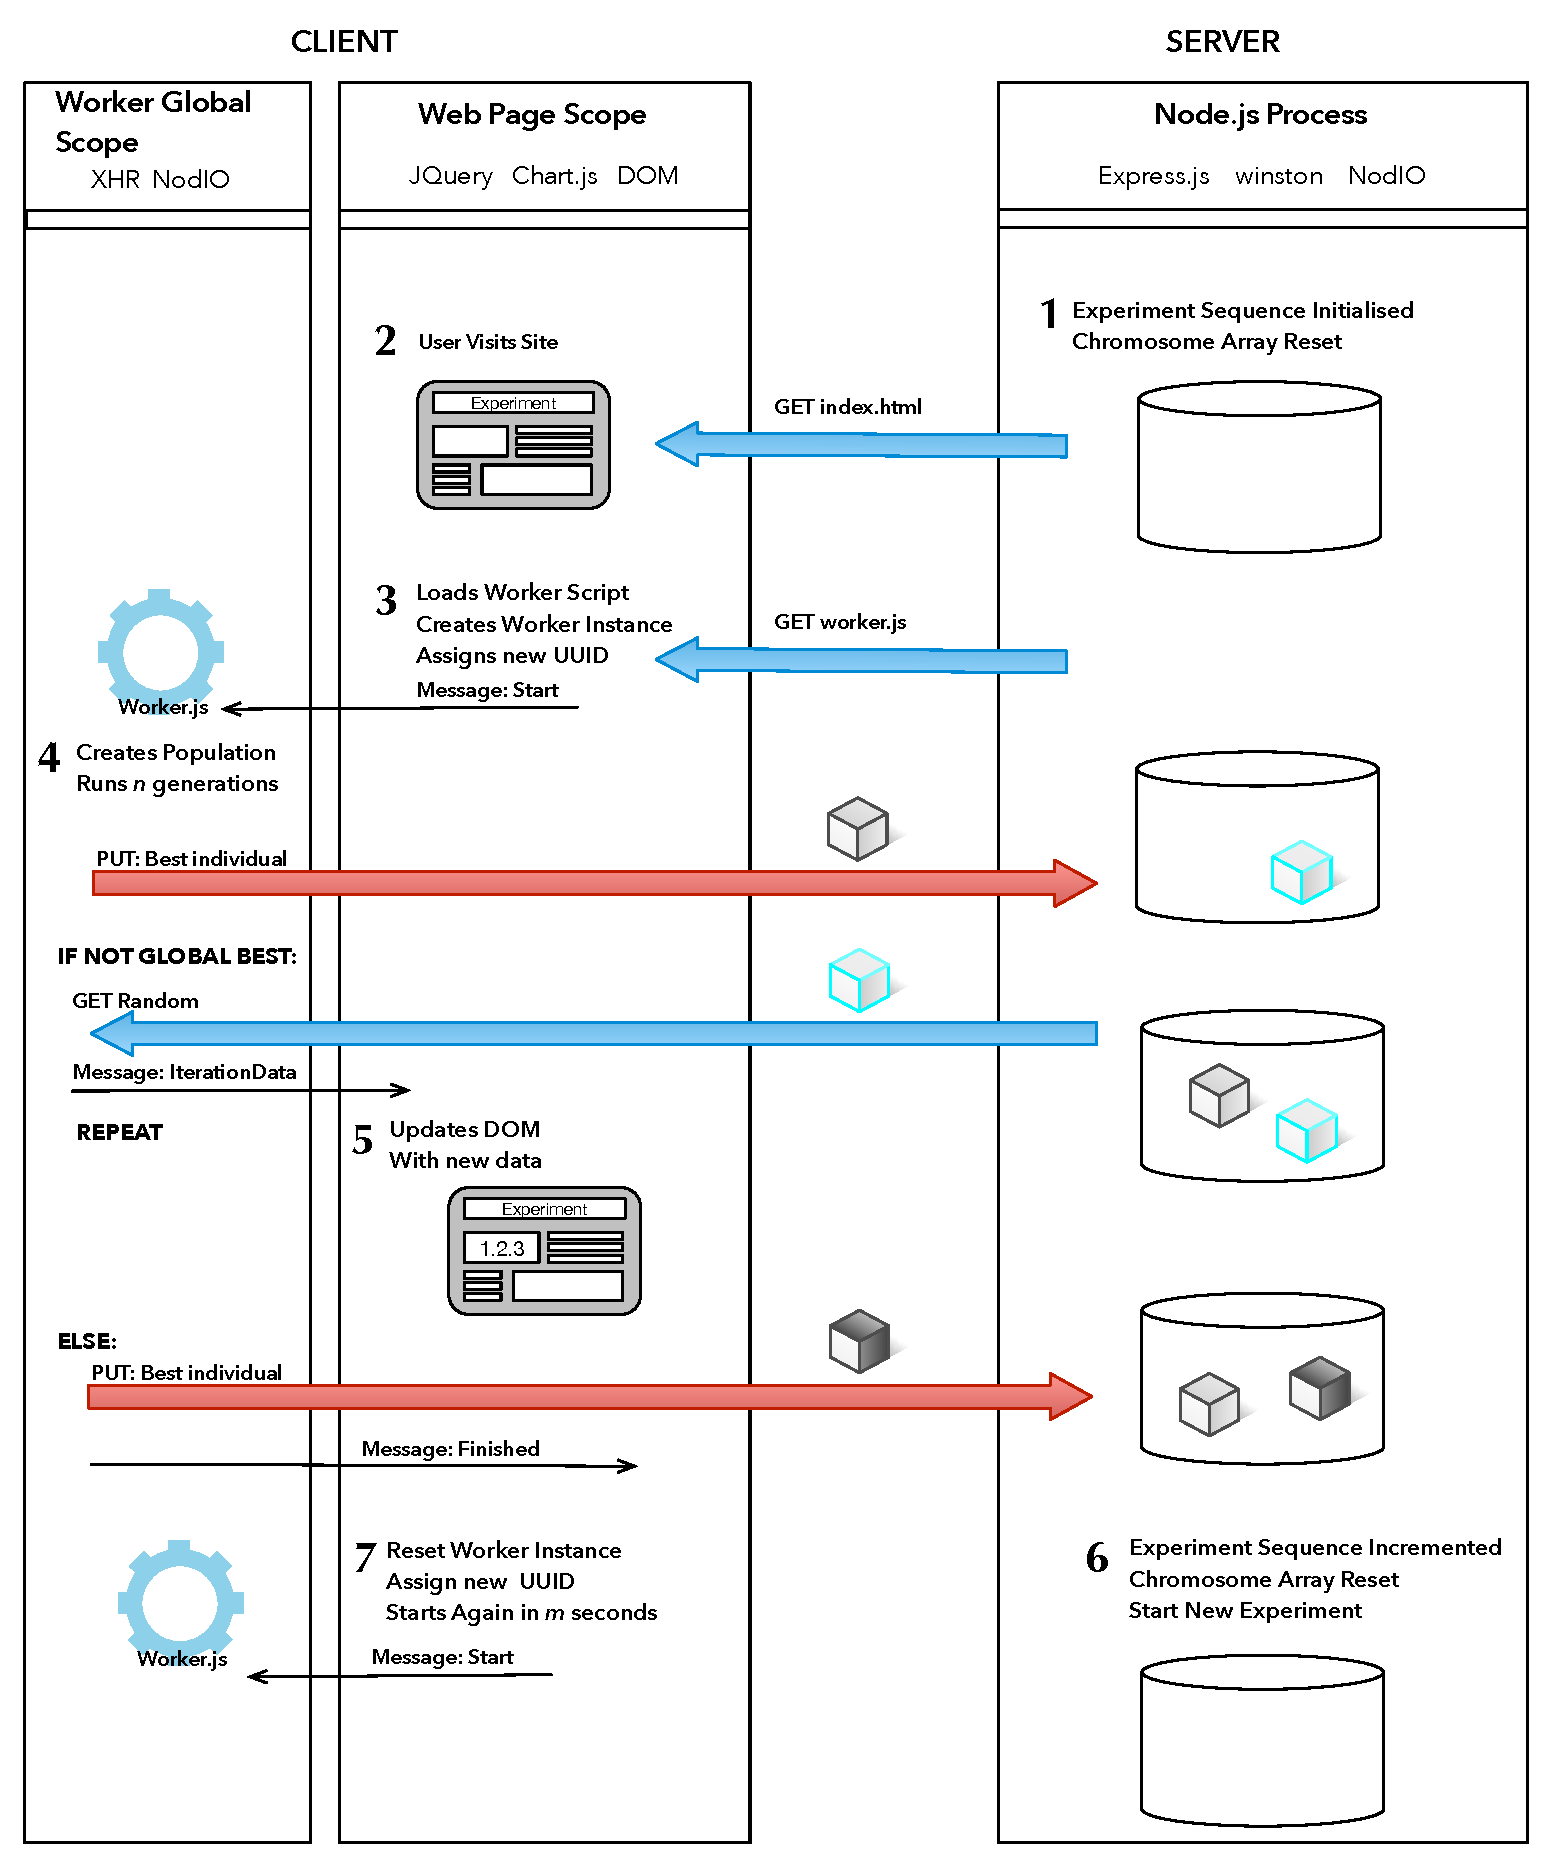
\includegraphics[width=4in]{Algorithm.pdf}
\caption{Description of the W$^2$ version of {\sf NodIO}. In this
  version, clients use Web Workers to run the evolutionary algorithm,
  with two of them per browser.}
\label{fig:system:w2}
\end{figure}
%
\begin{table*}[!htb]
\caption{Summary of {\sf NodIO-W$^2$} and comparison with the previous
  experiments, which have been aggregated to compute central measures. \label{tab:summary:ww}}
\begin{center}
\begin{tabular}{l|ccccccc}
\hline
Date & Median \#IPs & Max \#IPs & Median time (s) & Median \#{\tt
  PUT}s & $<$ 69s & $<$ 3.46s & Inter-experiment correlation\\
\hline
{\sf NodIO} & 5 & 29 & 123 & 14 & 37.43\% & 3.40\% & 0.10 \\
{\sf NodIO-W$^2$} & 4  & 16 & 7.36 & 40 & 89\% & 36.90\% & 0.4336061 \\
\hline
\end{tabular}
\end{center}
\end{table*}

The sequence of events happens as follows:
\begin{enumerate}
\item First the {\sf NodIO} process is started in Node.js. As part of the
initialization procedure, the sequential number of experiments is initialized and a log
file is created. The shared pool implemented as an array is reset.
\item A volunteer follows the link of the experiment triggering a GET HTTP
request, then the page is loaded.
\item The main script renders the page and creates the worker instance. In
order to create a dedicated worker instance, another GET request is sent to the
server, then the client receives the second worker implementation script.
Each worker instance executes over time one or more evolutionary algorithms
{\em islands}. Each island starts with a random population and it is assigned a
universally unique identifier (UUID). The UUID is included in each of the HTTP
requests sent to the server.
The initial parameters for each island
can be distinct. Once the worker is created and the parameters have been set,
a message is sent to the worker to start the algorithm.
\item The worker first creates the population following the previously
specified parameters. Once the population has been initialized, the EA
generation loop is started. After {\em n} generations the state of the population
is evaluated. The chromosome with the best fitness is sent to the shared
population with a PUT HTTP request. If the best fitness is not the global best,
the EA loop must continue, but first a chromosome is randomly selected from
the shared population. The current generation number and the best
chromosome are also sent to the client's main thread in order to update the DOM to
display the current state of the island (described next). These messages are
all asynchronous, so the EA loop of
the worker continues even before a message is received by the target. If the best fitness is a global best, the best
chromosome is sent to the server and the loop ends. A message is sent to the
main thread indicating that the best individual has been found.
\item The main thread receives messages from workers as events handled by
a callback function. When an iteration message is received, the page is
updated by displaying a dynamic plot of the generation number and best
fitness, and a representation of the chromosome is also generated.
\item When a global best is received from an island, the current experiment
ends, the experiment number is incremented, and the population array is reset.
\item When the main thread receives a message indicating that a worker has ended the EA
loop, that worker is reinitialized. The worker process is not ended, to
avoid the start-up cost, only the parameters and population are reset and a new UUID
assigned.
\end{enumerate}
%
\begin{figure}[!htb]
\centering
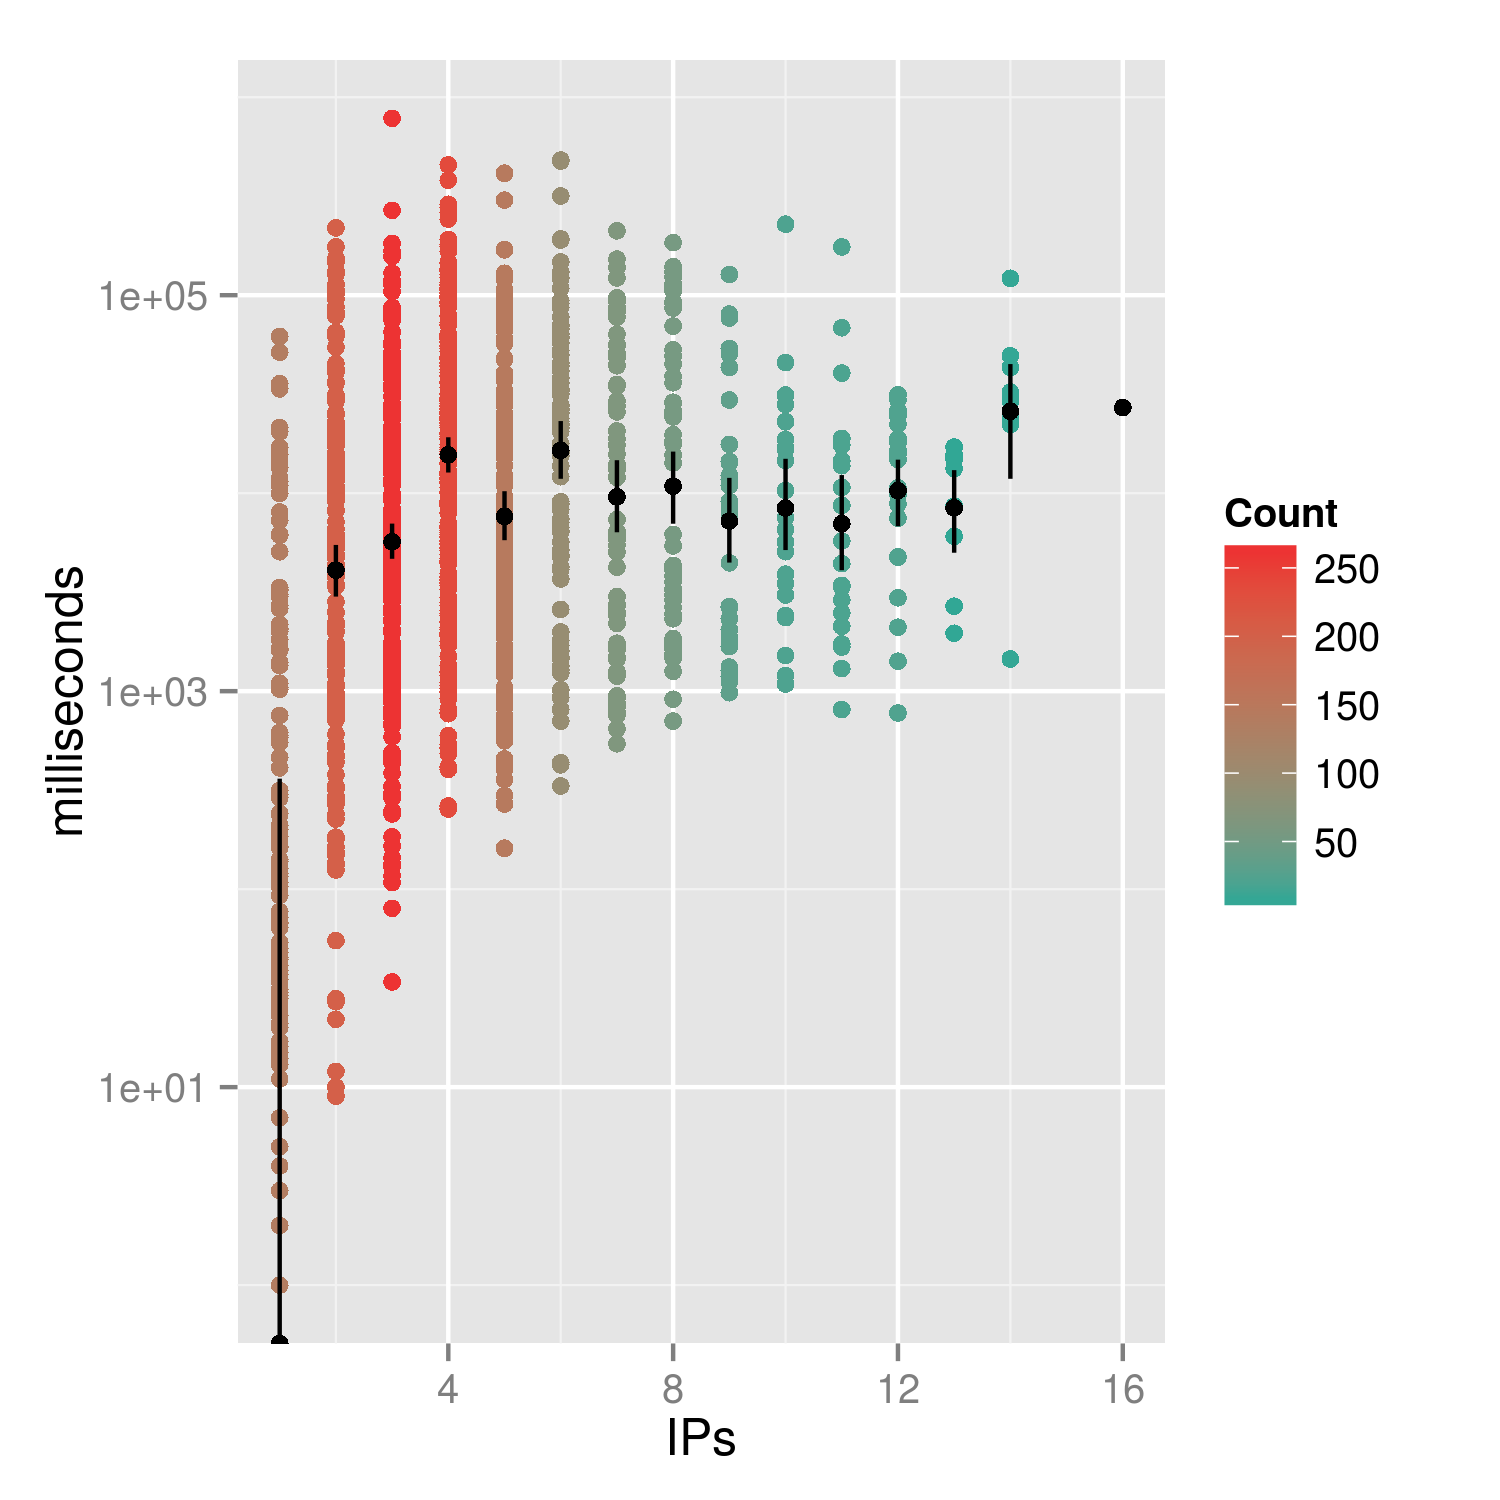
\includegraphics[width=0.9\linewidth]{ips-time-ww.png}
\caption{Time employed in every experiment vs. number of IPs (in
  abscissas). The red dot and line show the average and standard
  deviation, the shade of blue the number of experiments with the same
  number of IPs. } 
\label{fig:ipstime:w2}
\end{figure}

The experiments were run in the same way as before, using several
Twitter announcements throughout several days by the end of July
2015. Eventually, more than one thousand experiments were completed in
a matter of days. A summary of results is shown in Table
\ref{tab:summary:ww}, comparing it with the aggregate of the results
obtained with the initial version of {\sf NodIO}. These results are
remarkably different, being similar only in the median and maximum
number of IPs, although in this case it would be combination
IP-worker, as we considered every worker as a unique IP. The median
number of seconds is almost 80\% better than the previous version, and
the median number of PUTs is three times better; this causes that most
of experiments take less time than one of the baselines, and one third
less than the second baseline. Thus, the conclusion in this case is
that we can obtain, through volunteer computation, a result that most of the times is better than we would by using a similar, non-parallel,
desktop setup, which makes this system suitable for massively
distributed evolutionary algorithms.
%
\begin{table*}
\caption{Summary of fit to Generalized Extreme Value (GEV) and Weibull distribution of
  the number of {\tt PUT}s per worker. \label{tab:puts:ww}}
\begin{center}
\begin{tabular}{cccc}
\hline
Distribution & Location $\mu$ & Scale $\sigma$ & Shape $\xi$ \\
\hline
GEV & 18.275 $\pm$ 0.83719  &  25.962  $\pm$ 1.22015 & 1.242   $\pm$
0.04746 \\
Weibull & ND & 75.11457519 $\pm$ 2.97470251  & 0.69714410 $\pm$ 0.01383976 \\
\hline
\end{tabular}
\end{center}
\end{table*}
%

However, it is interesting to note why this is so, and the first hint
is the inter-experiment correlation between the number of IPs in
successive experiments. While before it was an unremarkable 10\%, it is
now more than 43\%, making the number of IPs in contiguous experiments
highly correlated. The main reason for this is the setup in {\sf
  NodIO-W$^2$}, which restarts an island after a solution has been
found and also that it keeps running even if the tab is not on the
foreground. This means that volunteers can leave the experiment
running for as long as they want and they will be contributing 
experiment after experiment, unlike the previous version, where they
stopped contributing after one solution was found. This is also
reflected in the number of PUTs, which is the number of generations
divided by 100; more than 50\% of the volunteers run the experiment for more than
4000 generations. All things considered, this means than there are
many more computers {\em simultaneously} running, leading to this
almost 5-fold increase in running time.


We are also interested in measuring the scaling properties in this
model, that is, the relationship between the number of IPs
participating in an experiment and the time it takes to complete
it. This is shown in Figure \ref{fig:ipstime:w2}, which displays every
experiment in terms of time (in milliseconds) vs. the number of workers participating
in it. Although there is not a clear trend, the graph seems to say
that the time needed for finding the solution in this evolutionary
algorithm does not depend on the number of workers participating in
it. This does not mean that it is independent on the number of {\em
  simultaneous} users, which is probably the case although it is more
difficult to measure. There seems to be a trend towards a decreasing
standard deviation in the time, with more volunteers adding both {\em
  robustness} to an experiment, and certainty in the time it is taking. However, more experiments would be needed to check this hypothesis.

\begin{figure}[!htb]
\centering
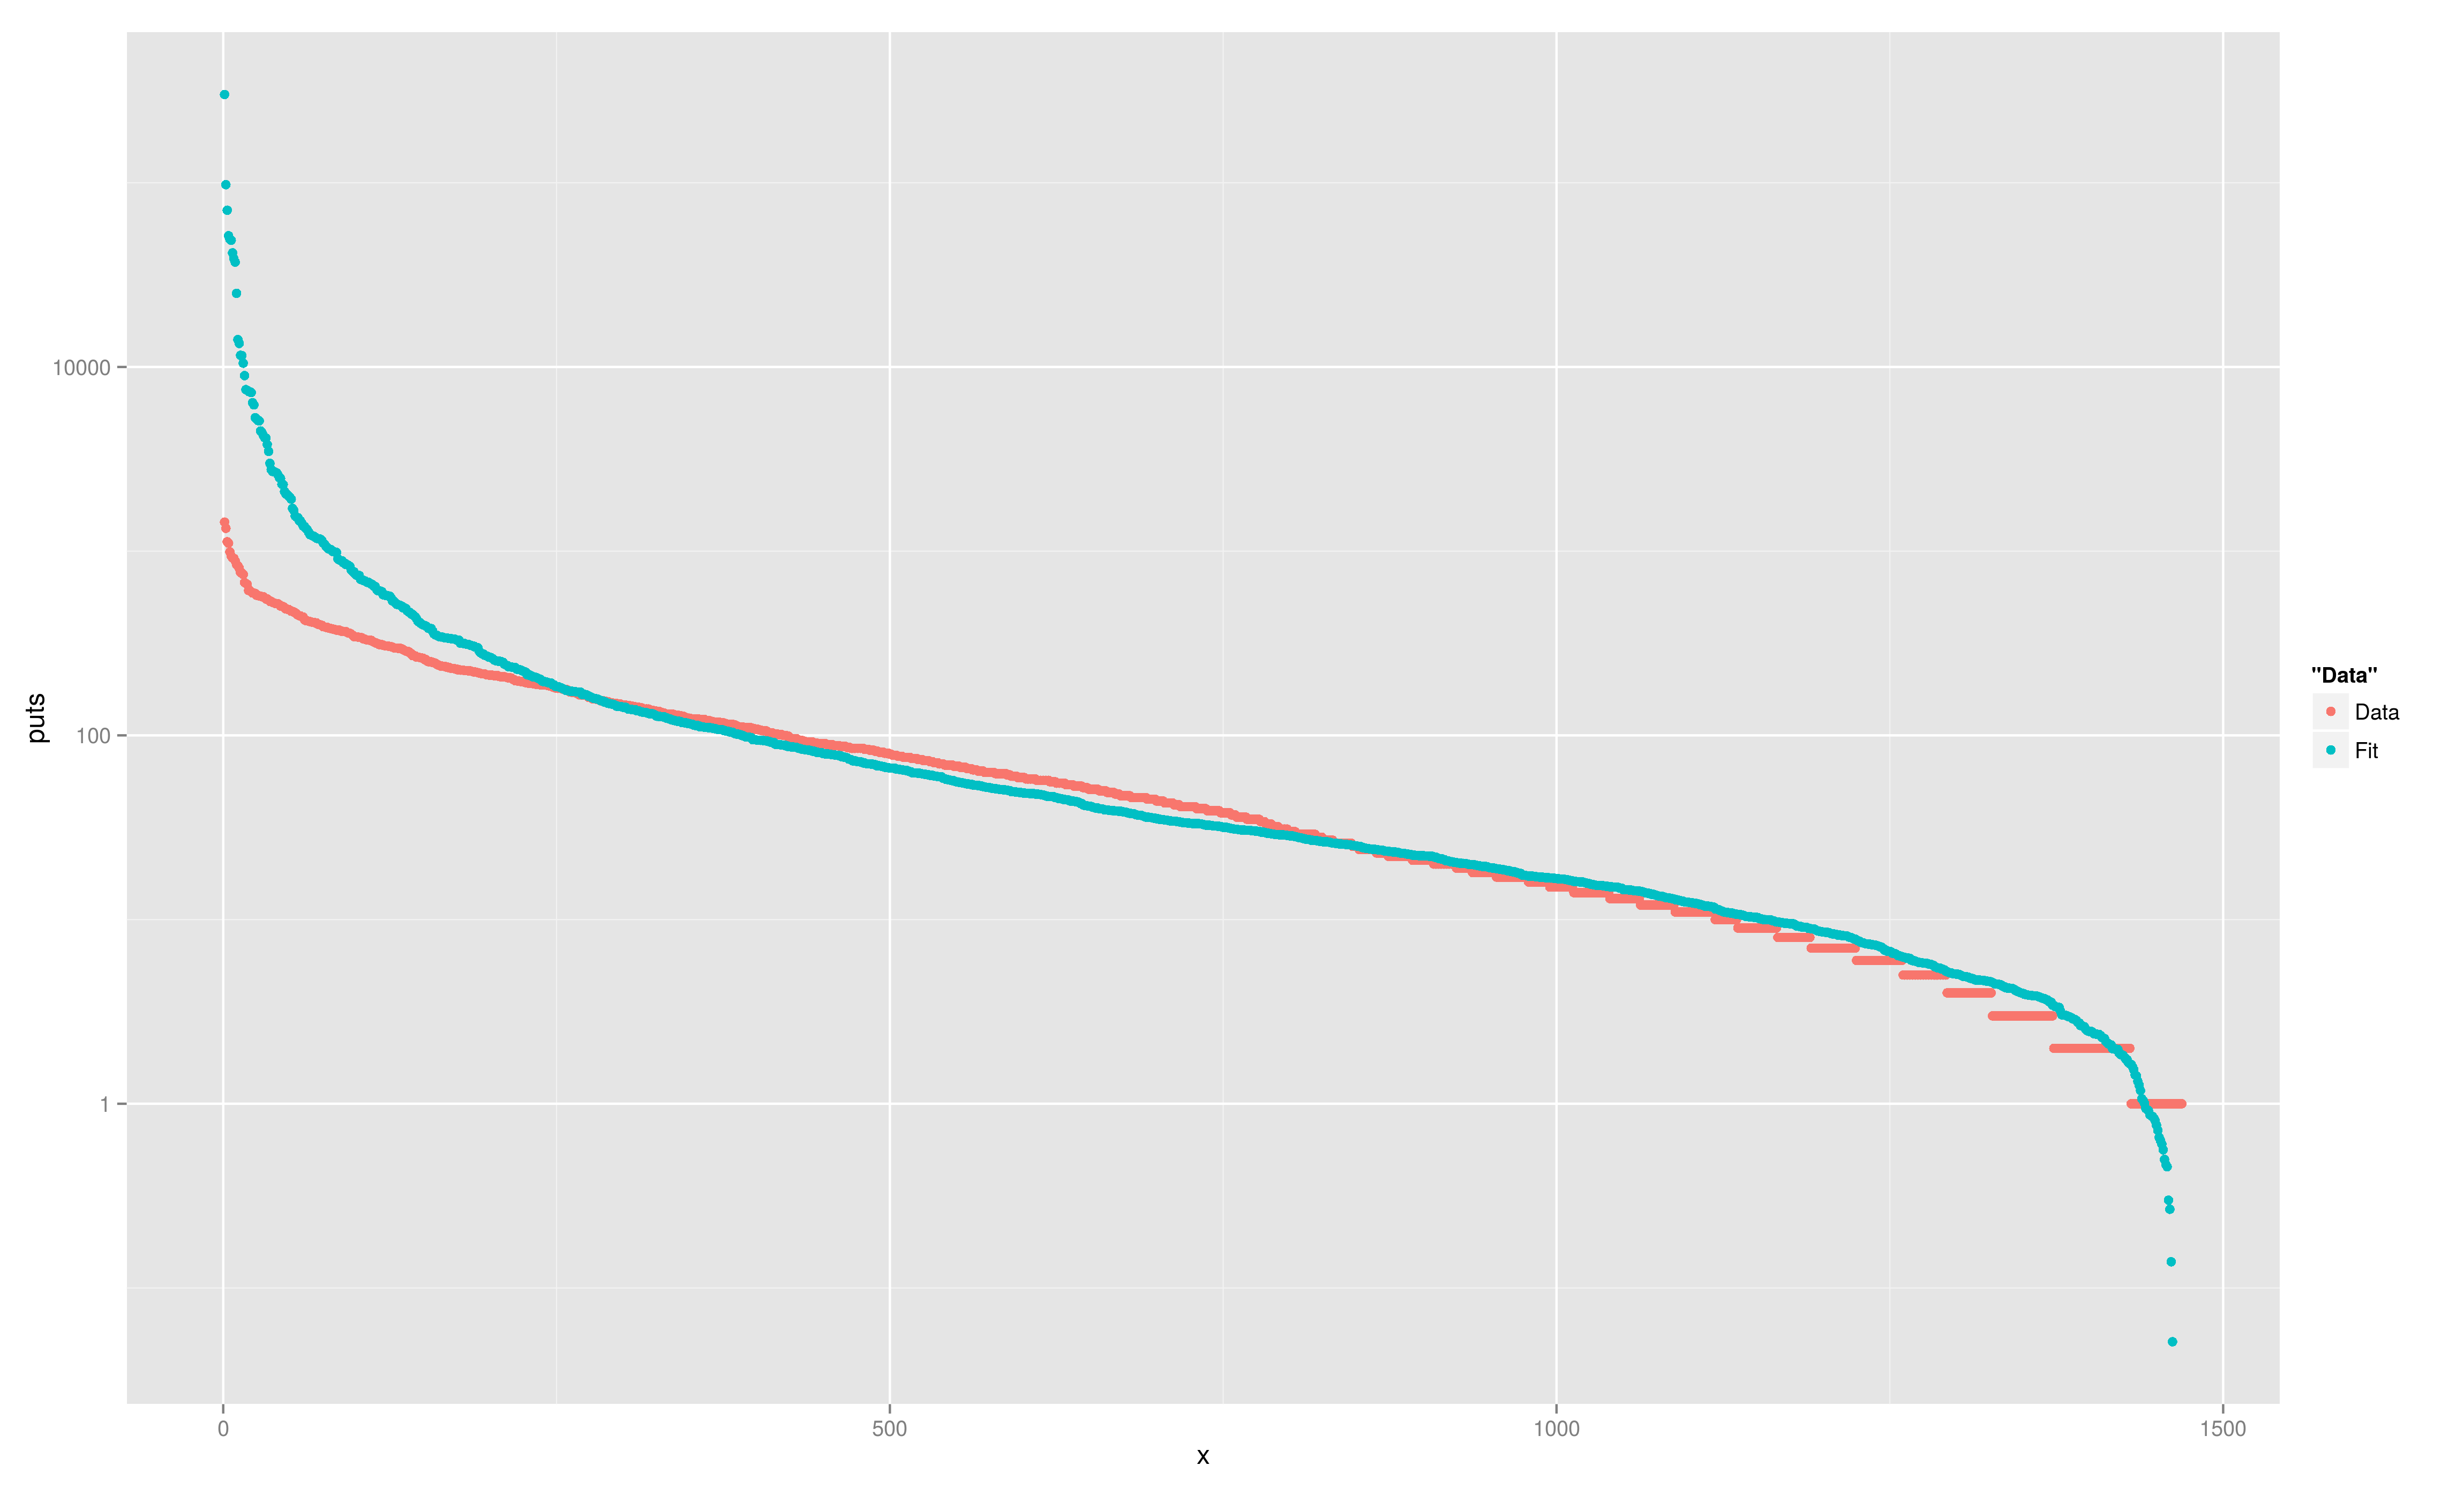
\includegraphics[width=0.49\linewidth]{gev-fit-ww.png}
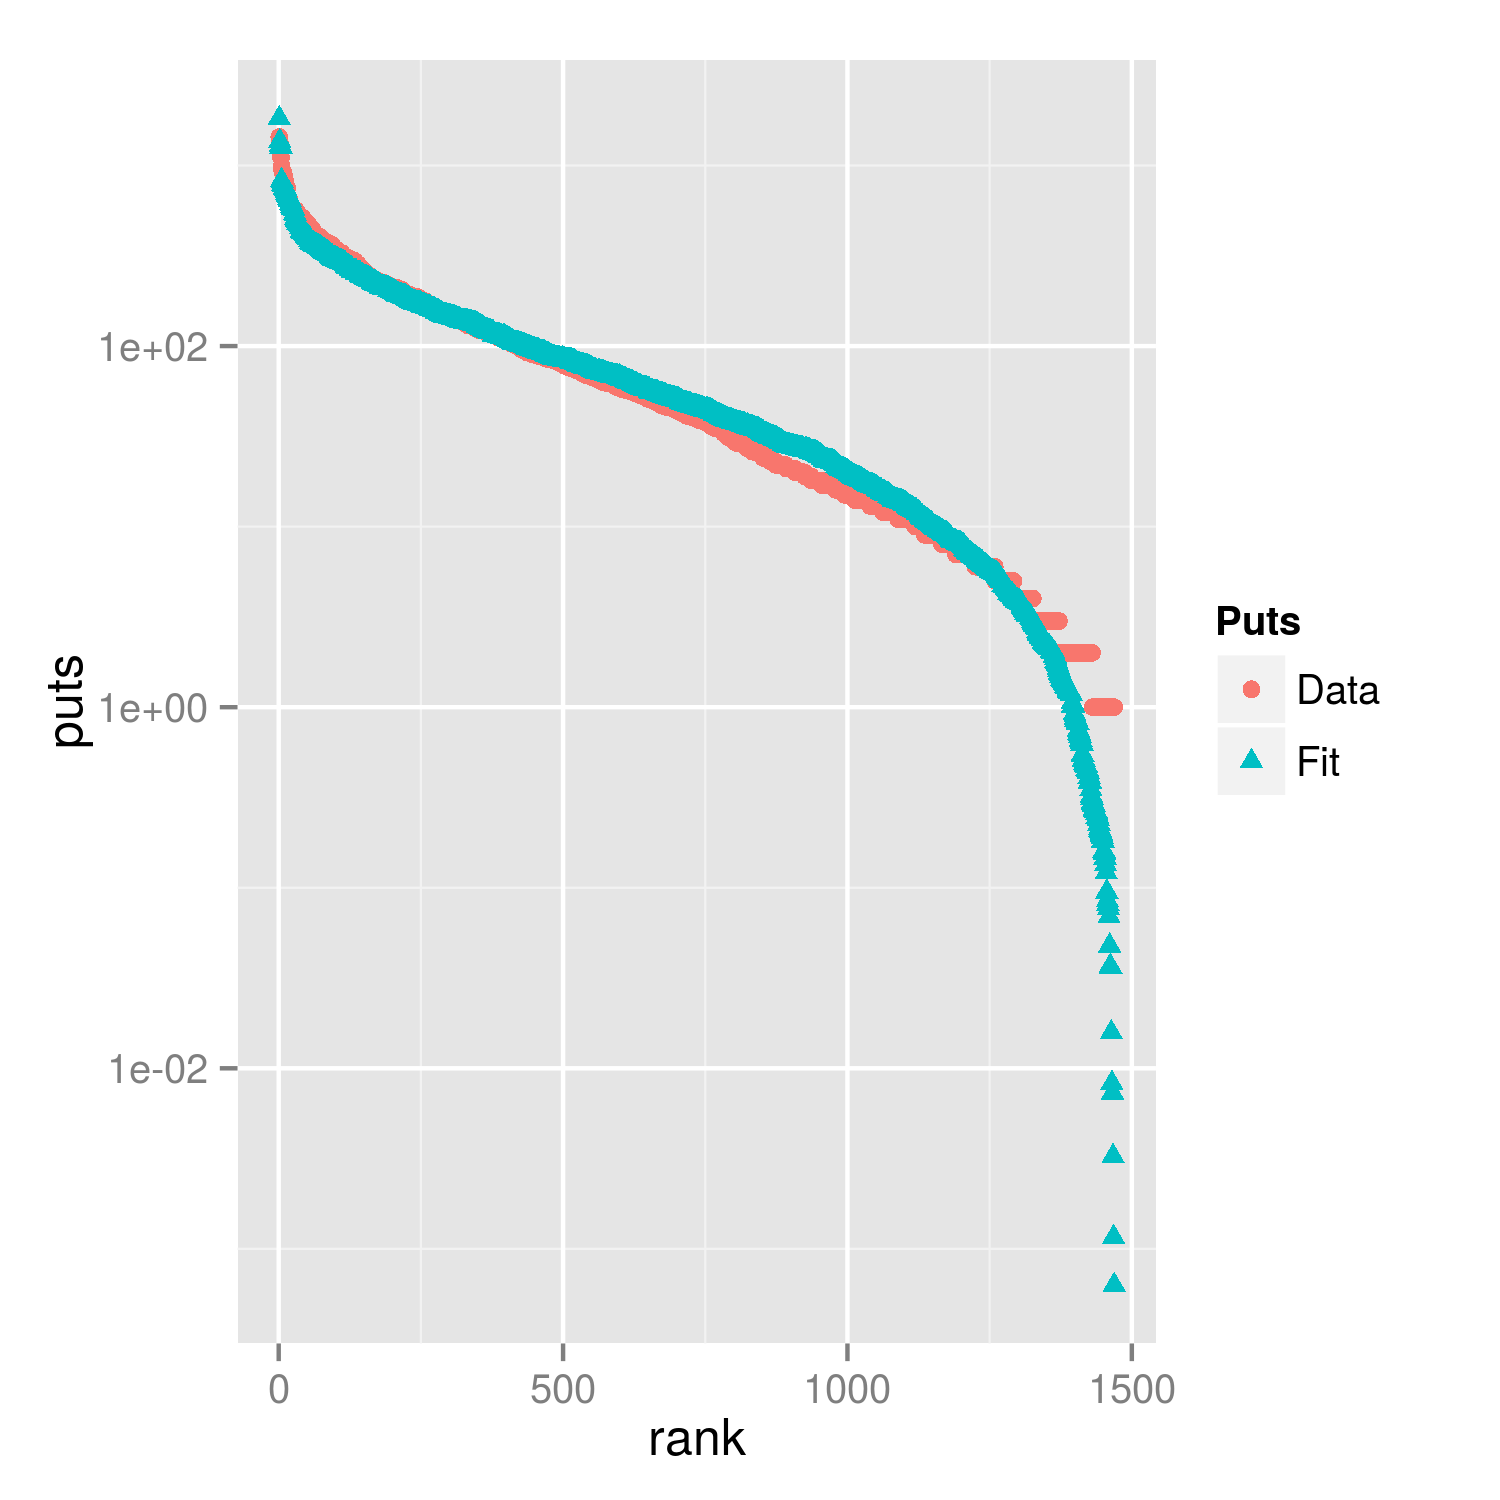
\includegraphics[width=0.49\linewidth]{weibull-fit-ww.png}
\caption{Ranked number of {\tt PUT}s per worker and GEV fit (in red, right) and Weibull (in red, left) for the {\sf NodIO$^2$} model.}  
\label{fig:gev:w2}
% File ../data/ips-puts.R
\end{figure}
%
As we did in the previous subsection, we have also fitted the number
of HTTP {\tt PUT}s per worker to a  Generalized Extreme Value (GEV) function, with the result shown
in Table \ref{tab:puts:ww}. Comparing this table with what we obtained
in the previous experiment, Table \ref{tab:puts:os}, we find higher values
for the location $\mu$ and scale $\sigma$ parameters, accounting for
the higher number of contributions per volunteer that has been
previously observed. However, the shape $\xi$ parameter is
substantially similar, with a {\em bell} shape leaning towards the
origin, indicating a pattern of a few users with many contributions
and many with few contributions. If we plot the model and the data
side by side, as shown in Figure \ref{fig:gev:w2} we see that the fit
is not so tight as in the previous case, with the model overestimating
the number of individuals with a high number contributions. This is
probably due to the fact that in the previous case, the user needed to
voluntarily reload the page to contribute the most generations, with a
{\em phase change} between the people that did so and the people that
just ran the experiment once until completion. In this case, however, the
user just needs to let it run, without that phase change and thus we obtain a
more {\em egalitarian} distribution of contributions, which rather
corresponds to a Weibull function, as shown in Figure
\ref{fig:ipstime:w2} (right hand side). The fitted parameters for this
distribution, shown in Table \ref{tab:puts:ww}, show a shape parameter
equal to 0.69, a value that is remarkably similar to the 0.5 value
found for time devoted to games in Chambers et
al. \cite{chambers2005measurement}. It is important to note that, in
this case, the number of PUTs made per client does not correspond to a
uniform amount of computation, since 100 generations with a random
population belong, in each case, to different number of
operations. In other words, the same number of PUTs will correspond to
different number of operations in each case. However, since clients
are also different and take a different time in each case, it is
difficult to ascertain how this might have an influence in the
statistical distribution.

In general, this second version of the {\sf NodIO} framework and the
single experiment performed prove that it can be the foundation for a distributed
high-server-performance evolutionary computation platform,
providing reasonable algorithmic performance and being, in general,
easy to use with a straightforward modification of the fitness
function. 


\subsection{$F_{15}:\frac{D}{m}$-group Shifted and $m$-rotated Rastrigin's Function}
JavaScript has been traditionally implemented as an interpreted
language not designed for the development of high performance
systems. On the other hand, current JavaScript  
virtual machines (VMs) are closing the gap, for instance the Google V8 
is an engine specifically designed for the fast execution of 
large JavaScript applications. In order to increase performance
V8 compiles JavaScript source code directly into machine code when it is first executed. 
There are no intermediate byte codes or an interpreter \cite{Gray:2009:GCM:1610564.1610565}.
JavaScript has gained popularity in server-side development using runtime
environments such as Node.js and is also used in desktop and mobile applications. 
%Mario: Creo que el párrafo de arriba sale sobrando
% (Paloma) Agree, I mean, it adds information but in case you have space problems... is ok if you start the section without it
To further evaluate how a current JavaScript implementation could be used by a
computer scientist to develop complex optimization problems,
a benchmark function, which was provided by the CEC2010 Special Session on
Large-Scale Global Optimization \cite{tang2007benchmark} is used in this section. 
The function is described next.


The basic Rastrigin's function is separable, and is defined as follows;
\begin{equation}
F_{rastrigin}(x)=\sum\limits_{i=1}^D [ x_{i}^{2}-10\cos(2\pi x_i)+10  ] 
\end{equation}
where $D$ is the dimension and $x = (x1, x2, · · · , x_{D})$ is a
$D$-dimensional row vector (i.e., a $1 × D$ matrix). Rastrigin’s function 
is a classical multimodal problem. Such problem is difficult since the number of local
optima grows exponentially with the increase of dimensionality. To make it 
non-separable, an orthogonal matrix is also used for coordinate rotation.
The rotated Rastrigin's function is defined as follows:
\begin{equation}
F_{rot\_rastrigin}(x)=F_{rastrigin}(\textbf{z}), \textbf{z}= \textbf{x} * \textbf{M}
\end{equation}
Where $\textbf{M}$ is  a $D \times{D}$ orthogonal matrix. The benchmark
emulates real-world optimization problems that most likely will consist 
of different groups of parameters with strong dependencies within
but little interaction between the groups. This issue is reflected in the benchmark 
by randomly dividing the objective variables
into several groups, each of which contains a number of variables. The parameter $m$ 
is used to control the number of variables in each group and hence, defining the degree
of separability:
\begin{equation}
F_{15}(x)=\sum\limits_{k=1}^\frac{D}{m}F_{rot\_rastrigin}[\textbf{z}(P_{(k-1)*m+1}:P_{k*m})] 
\end{equation}
For the benchmark $D = 1000$, Group size $m = 50$, $\textbf{x} = (x_1, x_2, \ldots , x_{D})$ is the
candidate solution, $\textbf{o} = (o_1, o_2, \ldots  , o_{D})$ is the shifted global optimum,
$\textbf{z} = \textbf{x} - \textbf{o}$ is the shifted candidate solution and
finally $\textbf{P}$ is a random permutation of $\lbrace1, 2, \ldots  ,D\rbrace$.

This optimization problem was selected because it is representative of the kind of
algorithms, data types, and structures employed in large scale optimization problems. 
The function was implemented in both Matlab and Java languages as part of the
Test Suite of the companion competition of the Special Session and to give competitors an idea of the
computational cost of the challenge, the runtime required for 10,000 function 
evaluations (FEs) for a particular configuration was published by organizers. The Java
implementation took 7596ms and the Matlab version 1115ms. The whole experiment had the value of
3,000,000 FEs as termination condition. Using the Java implementation as
a guide, the function described above was implemented to compare the performance of JavaScript against
both implementations, again using the time required for 10,000 FEs. 
Before discussing the setup and performance results, certain details of
the implementation in JavaScript are presented to give readers an idea of 
how practical and mature this language is for developing complex mathematical functions.

\begin{itemize}
\item {\em Randomize} Both Matlab and Java programs rely on a 
Java Randomizer library for the 
randomization of the shift vectors and matrices used by the function.
The library includes the generation of pseudorandom Gaussians of type
double and uniformly distributed integers. Generators use a single
{\tt long} seed. In order to implement the same functionality in
JavaScript, the library {\tt random-js} was used, as there are inconsistencies 
in the implementation of the standard {\tt Math.random()} between engines
and also their results are non-deterministic. 
The library {\tt random-js}, implements a Mersenne Twister algorithm producing 
consistent results across all JavaScript VMs.
\item {\em Timing functions} In order to compare the performance of 
each implementation, an accurate and consistent way of measuring 
the runtime of functions is needed.
In JavaScript the {\tt Date class} is often used 
to measure execution time, but has the limitation of having a maximum 
resolution given in milliseconds.
In order to measure the runtime intervals with a higher precision two functions
where used: for Node.js we used the native {\tt process.hrtime()} function
which returns a high-resolution measure in a {\tt [seconds, nanoseconds]}
array, and for measuring in the browser the {\tt Performance.now()} function was called,
which uses floating-point numbers with up to microsecond precision. 
A drawback found is that the {\tt Performance.now()} function is only implemented
in Firefox and Chrome browsers. Both functions are independent of the system clock. 
\item {\em Tools} An important consideration when choosing certain language to write non-trivial programs is the availability of development tools. While developing
the experiments, we used a comprehensive set of developer tools available for both
browsers and desktop. These tools included package managers, debuggers, logging libraries, 
network monitors, editors, and even debugging of the multi-threaded execution of Web Workers.
Although the fact that developer tools vary from browser to browser supposed a drawback, they all have the same functionality.
\item {\em Data Types} JavaScript uses floating point numbers with a 
limited precision of 64 bits that partially implement the functionality of
the {\tt StrictMath} library used by the Java implementation. If more precision
is needed, developers could use {\tt math.js}, an extensive math library with
support for matrices and big numbers.
\end{itemize}

We found that the JavaScript ecosystem is mature enough for developing non-trivial 
code, but developers have to consider the differences between VMs implementations
and therefore use certain libraries in order to increase the precision and repeatability of
algorithms. As for the performance of JavaScript against Java and Matlab
we conducted first the basic test described earlier in a 3.7 GHz Quad-Core
Intel Xeon E5 processor running OS X 10.10.5, 
using Java(TM) SE Runtime Environment (build 1.8.0\_25-b17), 
MatLab version R2015a for Mac OSX, Node FrameWork version 0.12.2,
Google Chrome Version 46.0.2490.86 (64-bit) 
and Firefox version 41.0.2. % (Paloma) Table here? Or at least the characteristics could be represented the same way as for the baseline experiment
 The performance of the time required for 10,000 FEs is presented in
Figure \ref{fig:f15_times}. In our test the Matlab implementation had the best
performance with an average of 935ms, followed by Java with
991ms. On the other hand, JavaScript took 32\% more time than Java with 1238ms in Chrome using a 
single Web Worker and 1,234ms using Node.js. % Are these results correct? JS=>1240ms and Node.js=>1,270ms ???
The results also show that there is not much difference between the Node.js
implementation an that of a
browser. There is also not much difference between running the code in the main thread or in Web
Workers. When running the experiment in Firefox a dialog alerted that the
script was taking too much time, showing that this
kind of processing is not intended for the main thread. Additionally, there is not much overhead
when running two
Web Workers in parallel as they took 1279ms each. This experiment
shows that JavaScript is viable as a language
language for developing complex mathematical functions an these can run in a browser
with acceptable performance. 
\begin{figure}[!htb]
\centering
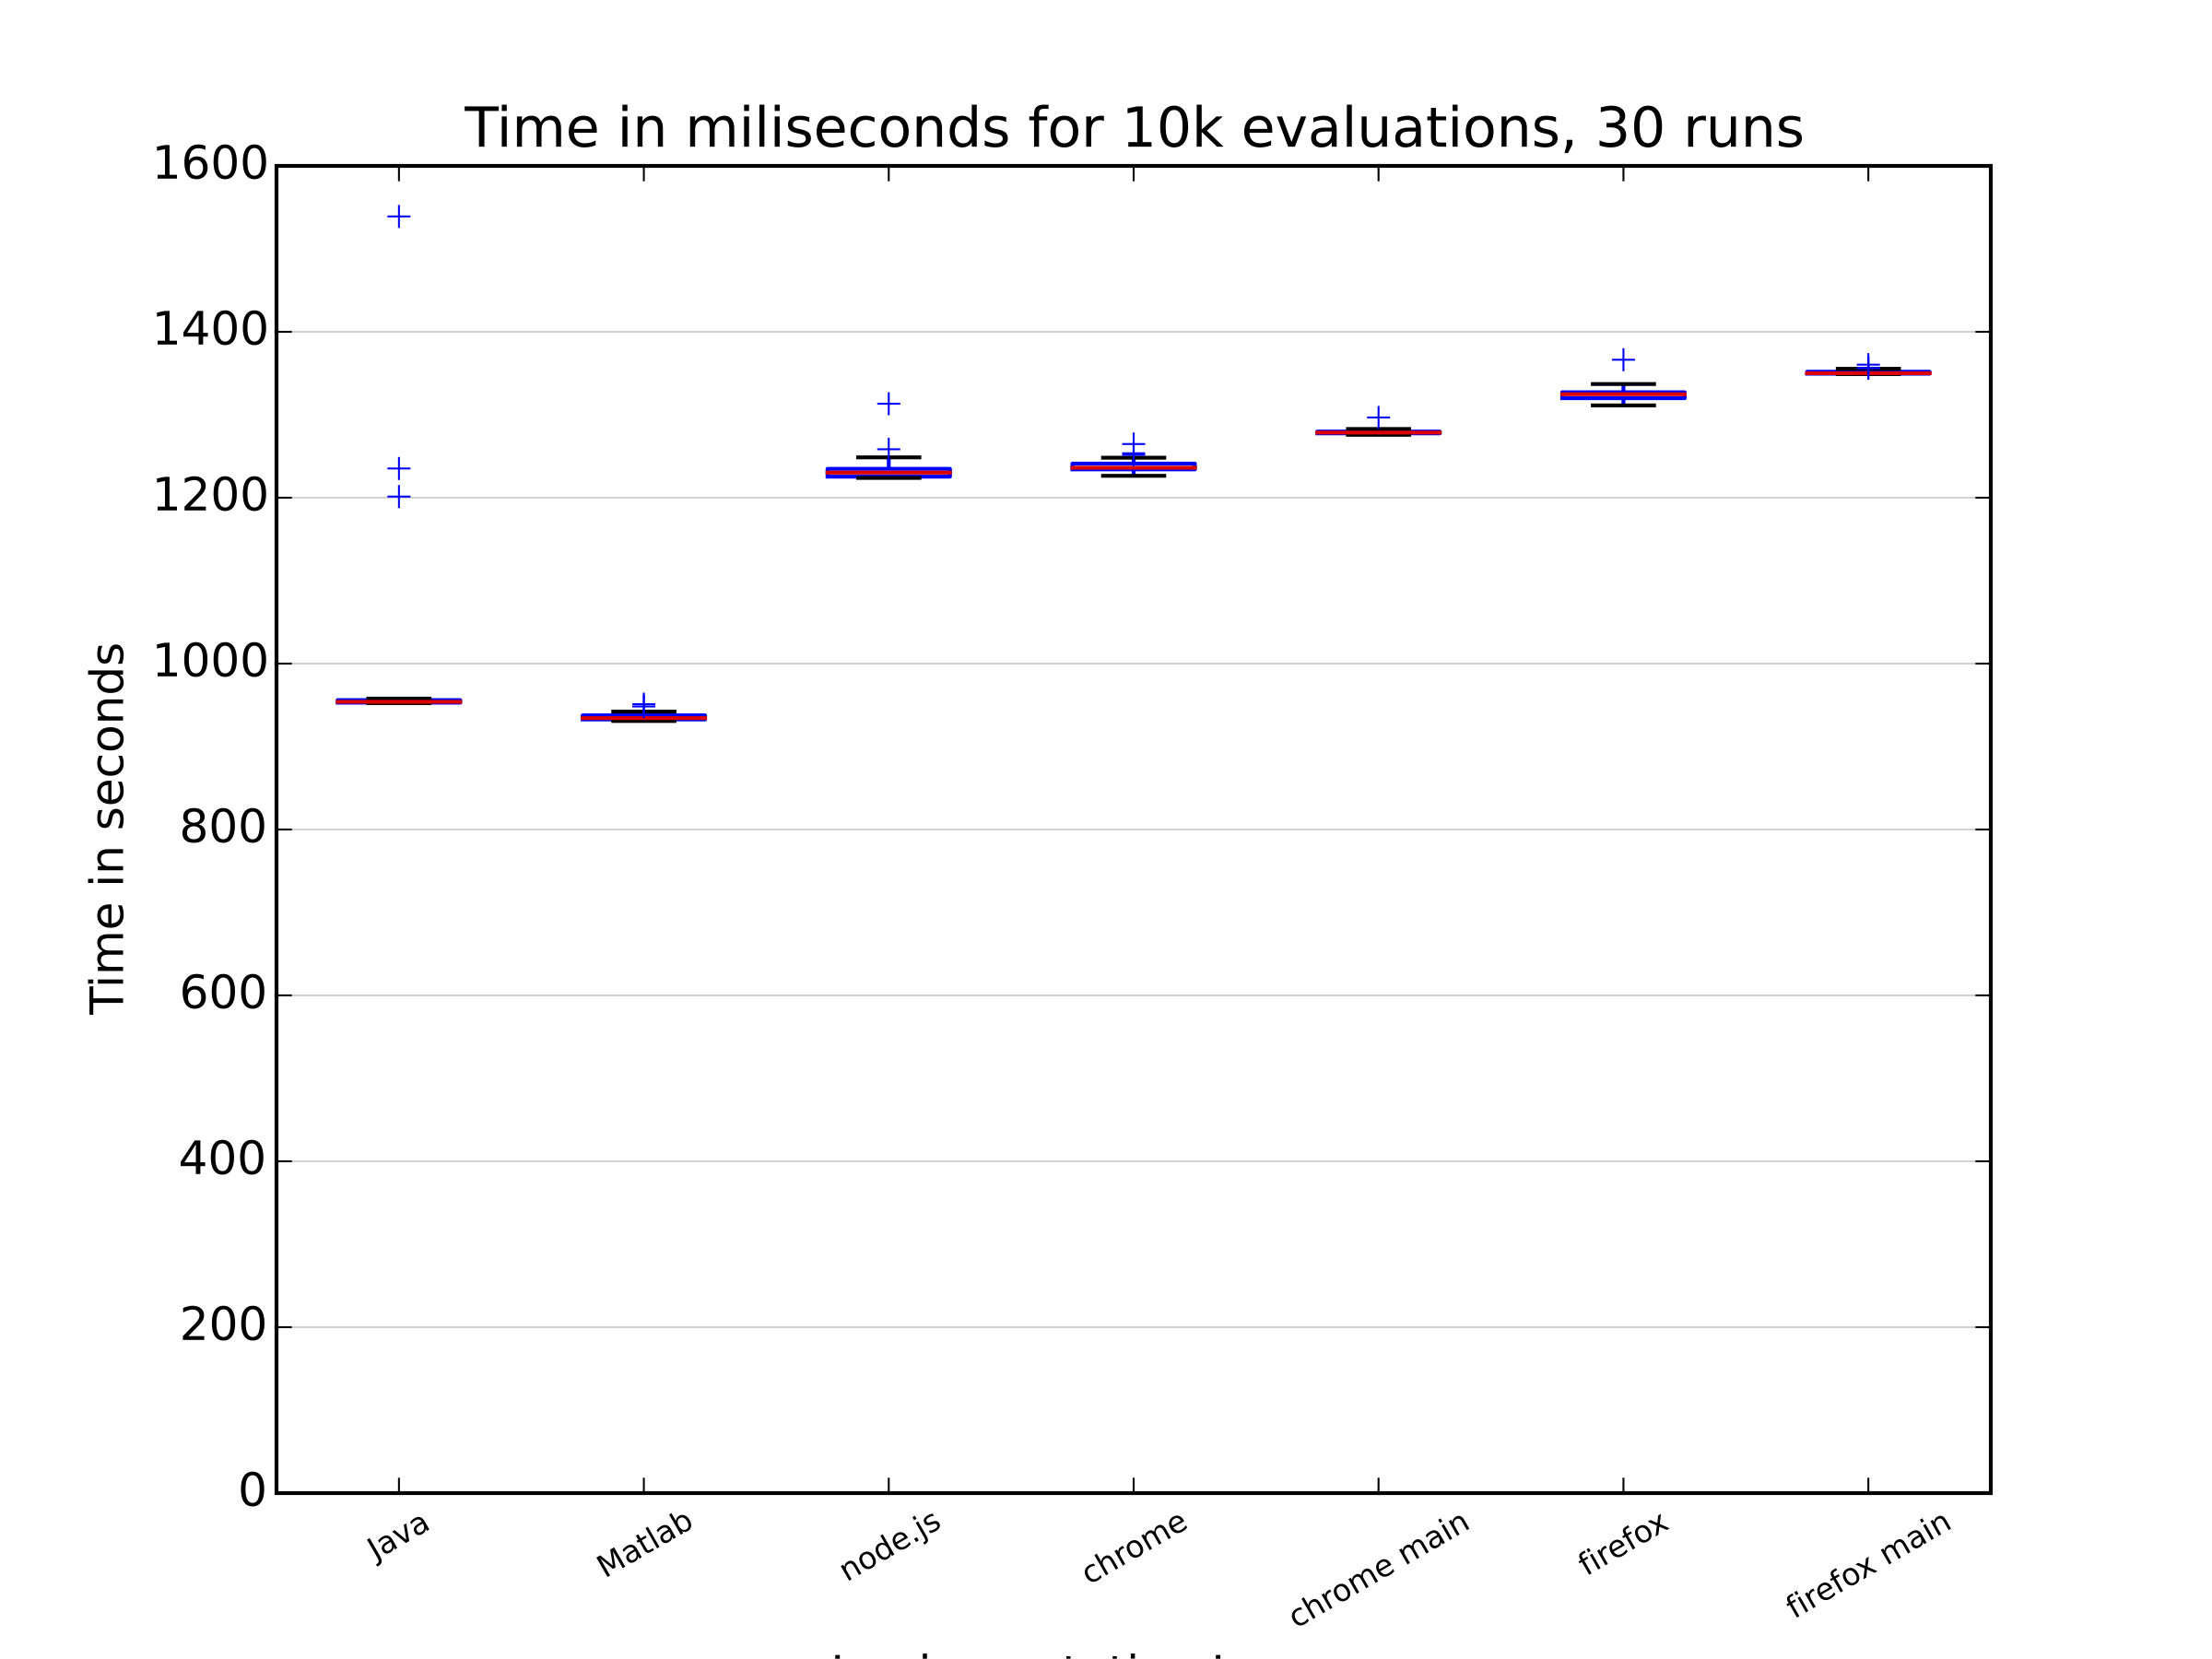
\includegraphics[width=0.9\linewidth]{f15_times.png}
\caption{ Runtime of 10,000 function evaluations (FEs) for $F_{15}$} 
\label{fig:f15_times}
\end{figure}

\subsubsection{Setup of Rastrigin's experiment in {\sf NodIO}-W$^2$ }
This experiment was deployed in a virtual private server with 512MB of memory
running Ubuntu OS version 14.04 and hosted in DigitalOcean.com. Unlike previous
experiments where the optimum was expected to be found many times, 
this problem was expected to run constantly for many days finding only
sub-optimal approximations. In order to achieve this, the only change needed 
in the system was to limit the number of chromosomes kept in the pool. 
Previously, every PUT request which included a new chromosome increased 
the size of the pool, in a long-running experiment this has to be avoided
in order to not exhaust the available memory. In this experiment the size
of a chromosome was 1000 double precision numbers, considering this
and the memory available in the server, the the pool was limited 
to 10,000 chromosomes.  In order to keep this size
constant a random chromosome was pulled out of the pool before inserting a
new one, when the pool was full. For this problem {\sf NodEO}'s {\tt chromosome-float} 
and {\tt classic-ea-float} modules were used. The parameters for the ea algorithm 
were tournament size = 3 and  population size = 500, returning exchanging a
chromosome with the server every 100 generations. Again two workers in each window.
As before, a few participation calls were published in social networks.

\subsubsection{Results}


%
\begin{figure}[!htb]
\centering
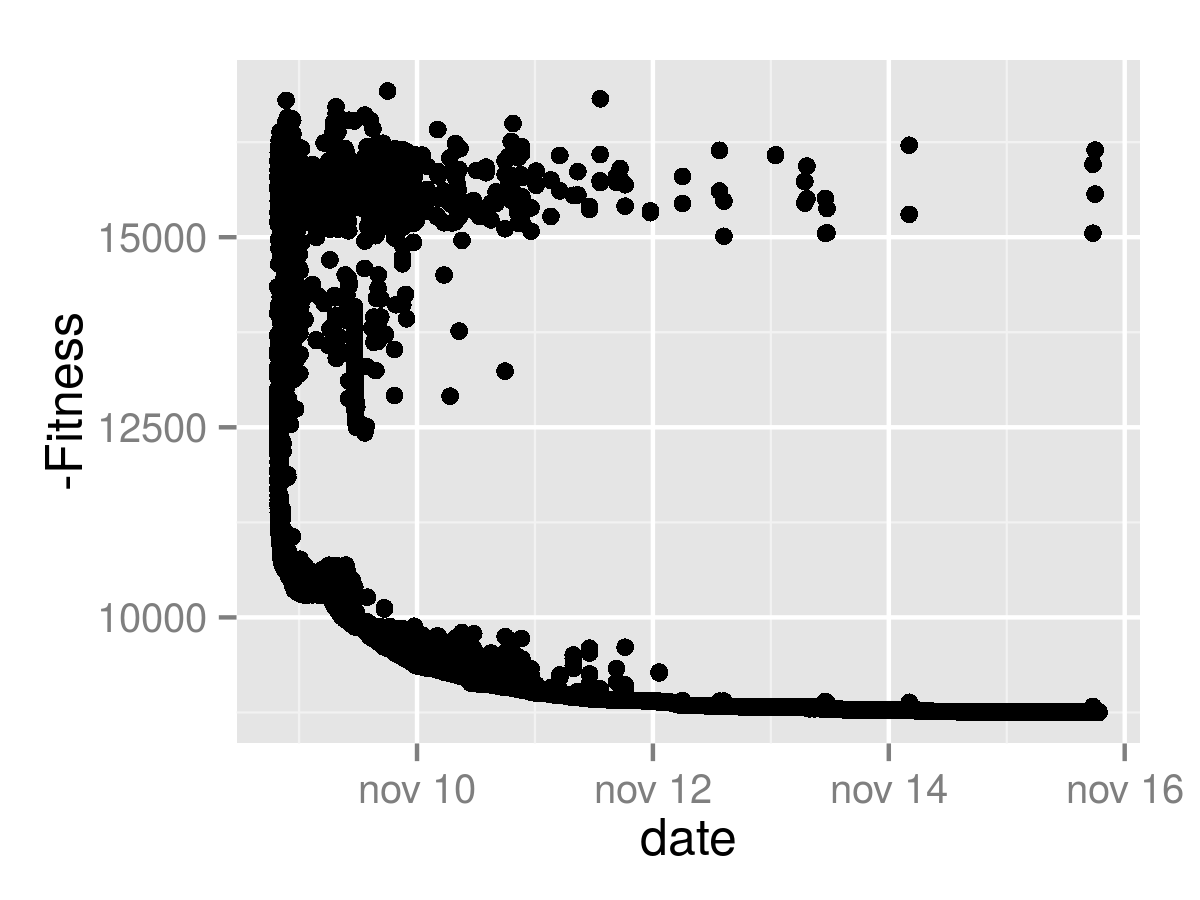
\includegraphics{rastrigin-fitness.png}
\caption{Fitness of chromosomes sent to the server pool along time in
  the $x$ axis.} 
% Plotted with ../data/plot-rastrigin-fitness.R
\label{fig:puts:rastrigin}
\end{figure}
%
\begin{figure}[!htb]
\centering
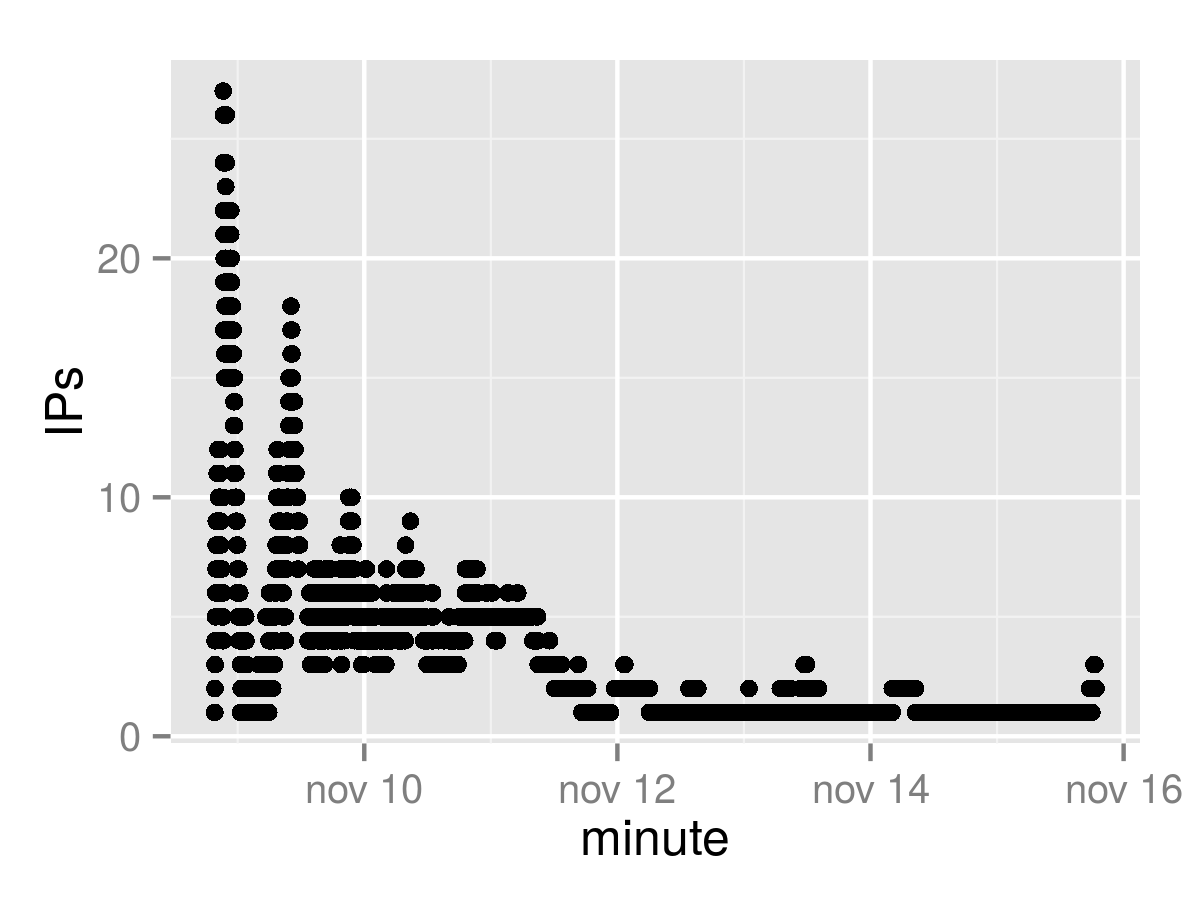
\includegraphics[width=0.49\linewidth]{rastrigin-IPs.png}
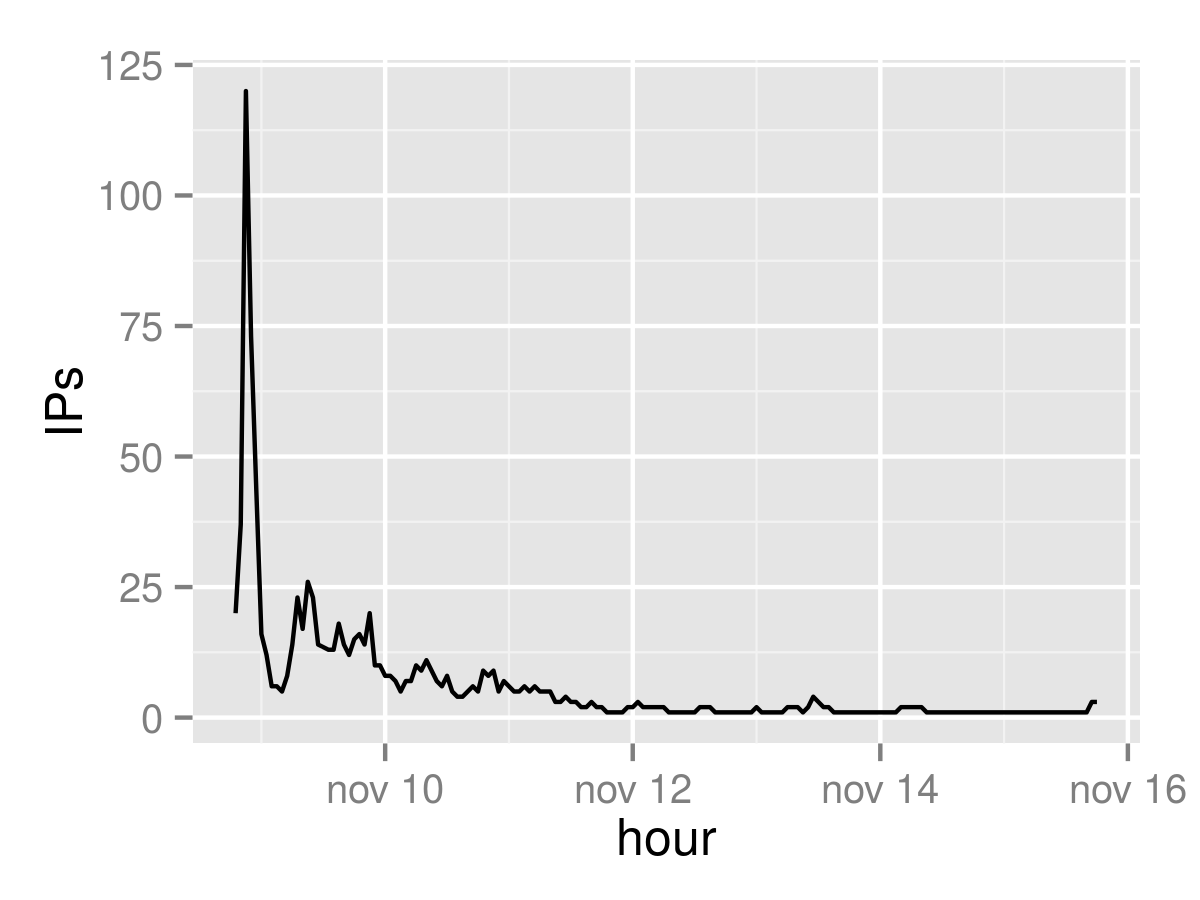
\includegraphics[width=0.49\linewidth]{rastrigin-IPs-hour.png}
\caption{Number of unique IPs participating in the Rastrigin
  experiment per minute (left) and per hour (right)} 
% Plotted with ../data/plot-rastrigin-IPs.R
\label{fig:ips:rastrigin}
\end{figure}
%
\begin{table*}
\caption{Summary of fit to Generalized Extreme Value (GEV) and Weibull distribution of
  the number of {\tt PUT}s per worker for the F15 (Rastrigin) function. \label{tab:puts:ww:f15}}
\begin{center}
\begin{tabular}{cccc}
\hline
Distribution & Location $\mu$ & Scale $\sigma$ & Shape $\xi$ \\
\hline
GEV & 35.759  &  343.336   & 9.877 \\
Weibull & ND & 29.002625061 $\pm$ 2.153034198  & 0.402393903 $\pm$ 0.007586468 \\
\hline
\end{tabular}
\end{center}
\end{table*}
%
\begin{figure}[!htb]
\centering
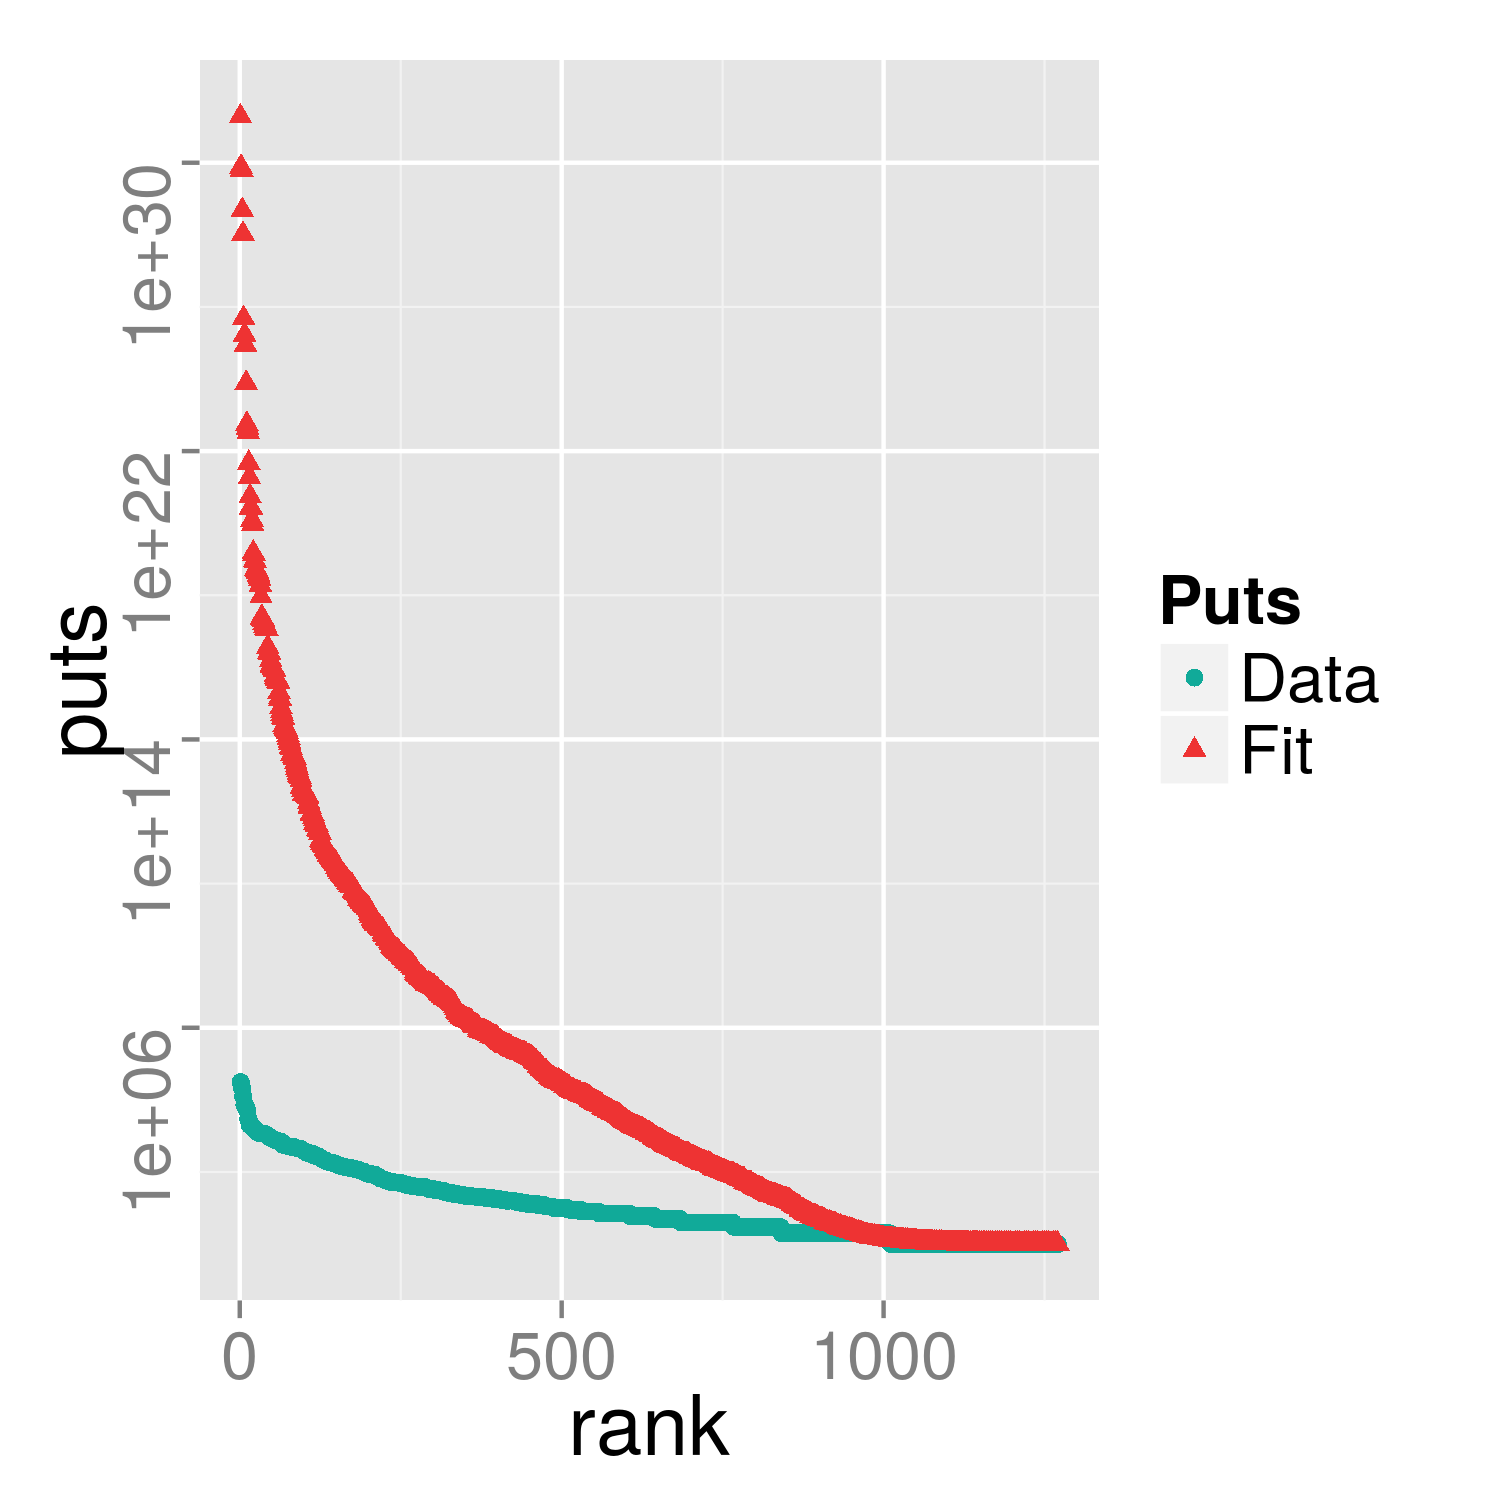
\includegraphics[width=0.49\linewidth]{gev-fit-ww-rastrigin-workers.png}
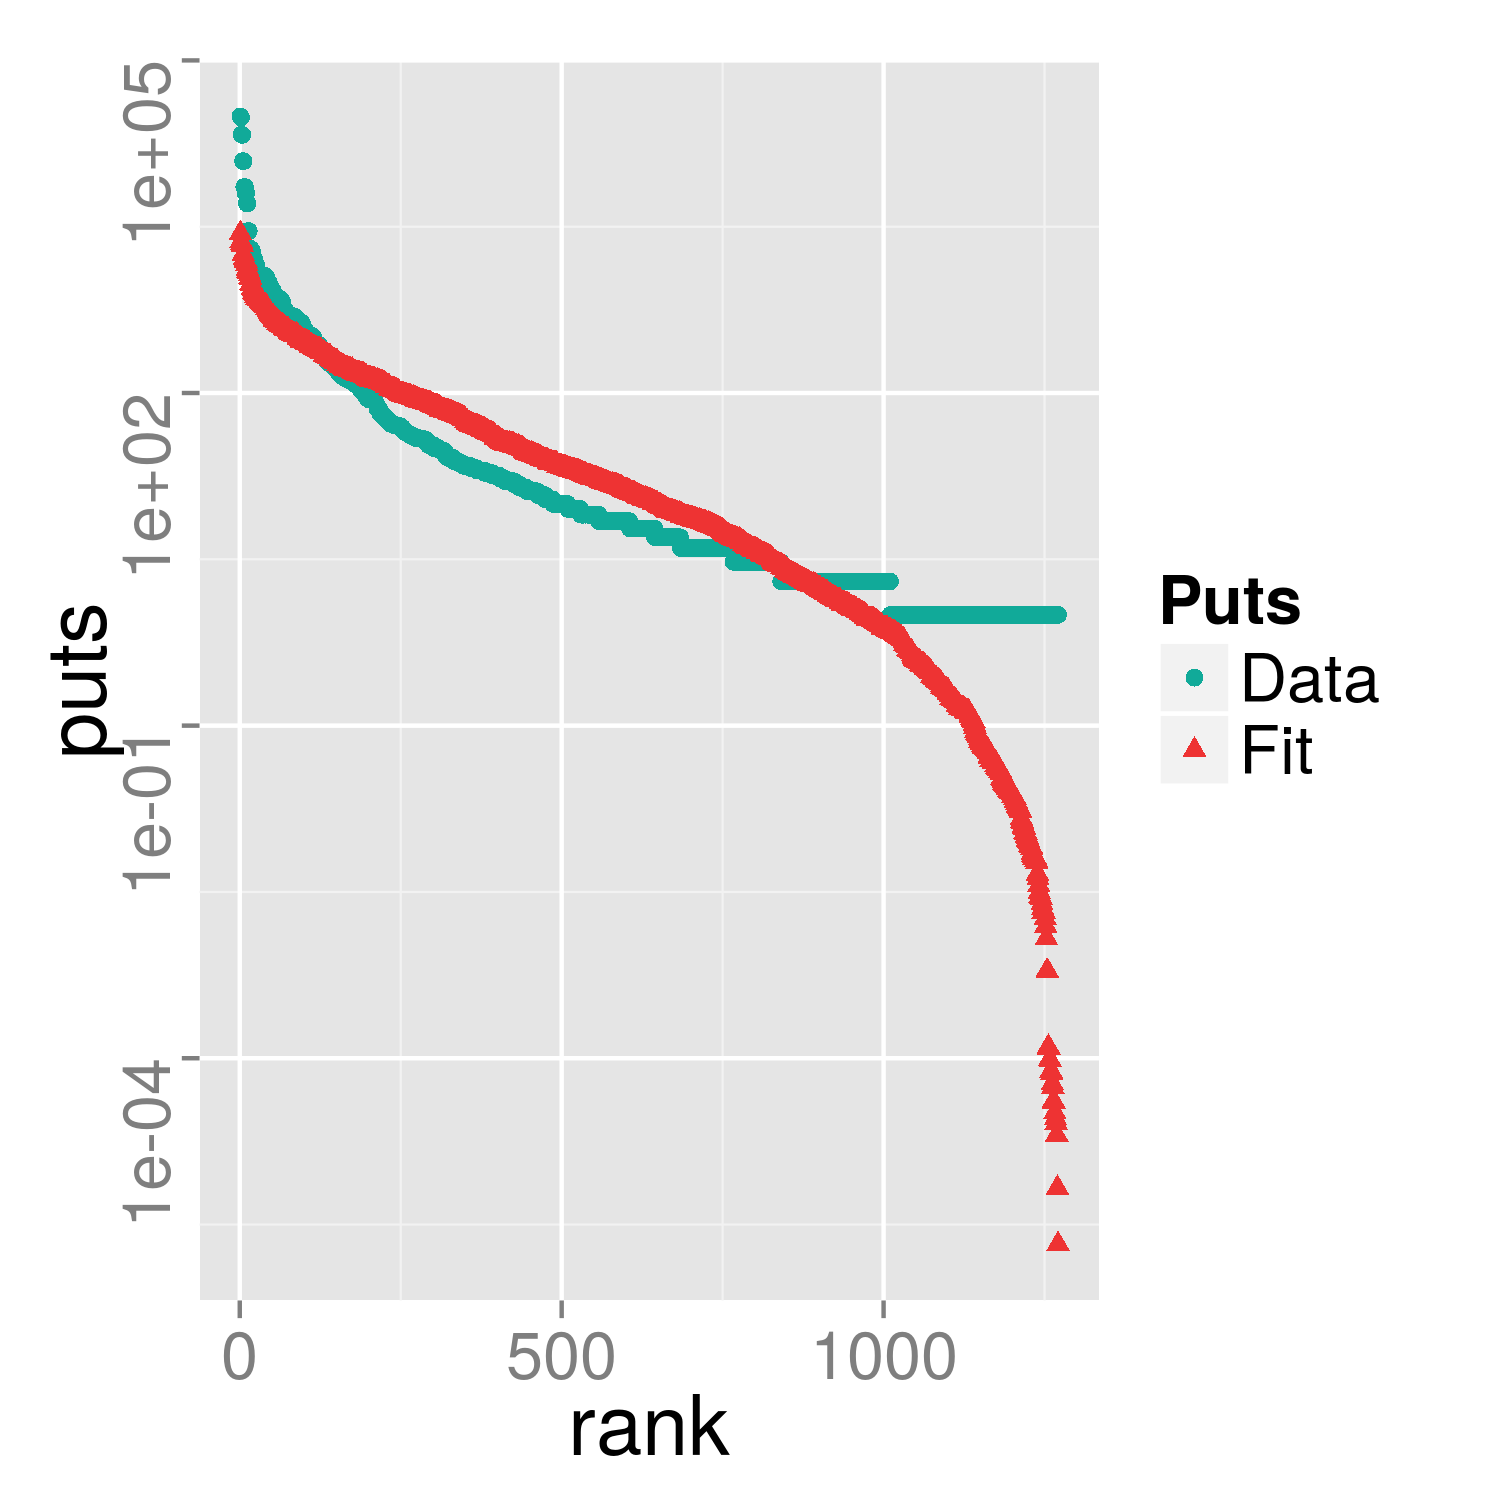
\includegraphics[width=0.49\linewidth]{weibull-fit-ww-rastrigin-workers.png}
\caption{Fit to GEV (left) and Weibull (right) of the number of {\tt PUT}s per worker for the F15 (Rastrigin) function.} 
% Plotted with ../data/ips-puts-rastrigin.R
\label{fig:fit:rastrigin}
\end{figure}
%

The results for this new experiment have been extremely interesting
and quite different from the previous one. The most important
characteristic that set this experiment apart from the previous one is
the fact that it did not find the solution for the time it was
running, instead lowering, little by little, the fitness until it was
disconnected. The fitness of chromosomes sent by clients is shown in
Figure \ref{fig:puts:rastrigin}, that shows two different parts: the
upper part, which represents the fitness of clients that have just
started evolution from a random population, and then the fitness of
those clients that have been already evolving for a while or obtained
a high-fitness individual from the pool and evolved from there, and
which managed to surpass the 9000 value by the end of the
simulation. It incidentally shows also the number of {\em new} nodes
coming: there is a dense {\em cloud} at the beginning, but the new
contributions keep thinning as the evolution progresses. 

This is in part due to the fact that the presence of nodes is not
constant, as shown in Figure \ref{fig:ips:rastrigin}, which plots the
number of unique IPs participating in the experiment per minute (left)
and hour (right). The two graphs have the same shape which matches
also the speed in which fitness is decreased in Figure
\ref{fig:puts:rastrigin}. At the beginning there are very few or only
one, but later one there are peaks of almost 30 unique machine a
minute; these peaks appear again when new announcements are made in
Twitter or any other social networks, to go down to a few remaining
nodes later on. It is interesting to note that, at the most, more than
100 unique nodes were participating in the experiment during one hour;
also that there are sustained peaks during a day of 6-7 computers
every minute. This is due to the fact that the computation is
asynchronous, but also to the fact that different computers stay in
the simulation for a different period of time. This period has been
plotted in Figure \ref{fig:fit:rastrigin}, that plots the number of
{\tt PUT}s per node, ranked by number, along with a fit to the two
distributions we have used before, GEV and Weibull; the parameters of
this fit are shown in Table \ref{tab:puts:ww:f15}. Unlike the previous
experiments, in which GEV fit was relatively good, in this case it is
quite obviously not. However, the fit to the Weibull distribution,
shown at the left of the image, is relatively good. As should be
expected, the shape and scale are different to the one in the previous
experiments with the Trap function, however, the shape is quite
similar (0.40 vs 0.69), being in both cases less than one, which
indicates a decreasing distribution of the same kind. In fact, the
difference in the scale parameter indicates that the difference
between the time devoted by a volunteer and the next is bigger in this
case. This is probably due to the fact that the duration of the
experiment is bigger, allowing for bigger differences in
behavior. While the first in the Trap function might have devoted a
few minutes and the second a few seconds less, the difference between
the first and second in this experiment might be in the scale of
hours. 

In general, this experiment confirms what was found in the others in
several aspects: first, there is a regularity in the distribution of the
time assigned by volunteers to it, second, there is a good and certain
amount of volunteers that will become part of the distributed
computer, in some cases up to one hundred; also, in some cases there
will be users that will spend several hours, two orders of magnitude
more generations in this case than in the previous one. There is a
clear influence of the time to solution: a short time means that every
experiment will only gather a few volunteers, but also that they will
stay only for a short time. A long time will make users stay for
longer, but if it takes too long, they will eventually lose interest. 

We will discuss this and the rest of the findings of the paper in the
conclusions. 

%---------------------------------------------------------------
\section{Conclusion}
\label{sec:conclusion}

In this paper two versions of a client-server architecture for volunteer and distributed
evolutionary algorithms that uses the browser and generated using {\sf
  NodIO}, based on the {\sf NodEO} evolutionary algorithm library have been
evaluated. Volunteers are {\em in the cloud}, as stated in the title,
since they are a {\em CPU as a service} for the persons running the
experiment. In fact, in this paper we have tried to put some figures
on the real size of that {\em cloud} and how it can be used standalone
if there is no alternative or in conjunction with other local or
cloud-based methods to add computing power in a seamless way through
the pool that NodIO creates. 

In order to establish a baseline performance, the evolutionary
algorithm was run in a desktop client-program written in JavaScript
using NodEO to solve the 40-trap function. The first experiments with
{\sf NodIO} proved that, although obtaining better performance than the
baseline was possible, it did not happen, mainly because of the
difficulty in carrying over volunteers to other experiments when the
one they were participating on was finished, shown in the low
correlation between the number of IPs in successive experiments. This
also resulted in a low number of generations allotted by users. 

In the second implementation, {\sf NodIO$^2$}, Web Workers
were used so that several clients per browser could be executed and
they could run in the background, so that the the number of
generations per user could be improved. The number of generations per
user increased to the point that baseline performance was improved in
most cases. The architectural changes led to a high correlation
between successive experiments, so that, even as the median number of
volunteers per experiment decreased, they were probably contributing
to the experiment at the same time, so that our objective was
achieved. In general, one of the first conclusions for this paper is
that the browser technologies should be used to its full extent so
that the user time is leveraged to its full potential, and this was
achieved with {\sf NodIO$^2$}. 

The second objective of this paper was to model the user behavior in a
first attempt to try and predict performance. As should be expected,
the model depends on the implementation, with contributions following
a General Extreme Values distribution in the case of {\sf NodIO} and a
Weibull distribution for {\sf NodIO$^2$}. These distributions are
close enough to each other and, in the second case, reflect the fact
that all time spent in the page is actually devoted to computing,
which is why the time spent (represented by the number of
contributions to the pool) follows a model quite similar to that found
for games or other online activities. The reverse might be true: if we
want to have returning users for the experiments, it is probable that
we should {\em gamify} the experience so that once they've done it
once, they might do it more times. In the spirit of Open Science, this
gamification might involve computing in real time data such as the one
presented in this paper and showing it in the same page. 

In general, linking and finding correlations between user choices and
performance is an interesting avenue to explore in the future. Even if
the three previous experiments were published in a similar way, one
obtained up to 5 times more total cycles  that the one with the least
number of cycles. It is also essential to obtain volunteers as
simultaneously as possible, so it is possible that the features of the
social network in terms of real-time use will also play a big
role. Even as it is difficult to create controlled experiments in this
area, it is an interesting challenge to explore in the future.

Although we think that, in general, the results presented in this
paper are independent of the problem chosen, it is true that even if
it is a difficult problem for evolutionary algorithms, it takes a few
seconds with the right settings to solve. This makes it difficult also
for this kind of asynchronous framework, but it would be interesting
to check the performance for other computationally demanding
tasks, especially ones that cover the middle ground between a problem
finishing in seconds or minutes (Trap) and weeks (Rastrigin F15). 
Besides, the two versions of the framework include as an
algorithmic variant using random population size. We do not think this
has had a big influence on the results and in fact this is not noticed
for F15, which is the second version tested but it would be interesting to
measure exactly what this influence has been. In general there are
many issues with the evolutionary algorithm implementation itself,
including using different, or adaptive, policies for inserting and
sending individuals to the pool as was done in \cite{araujo2008mam},
using different policies for population initialization, and also the
incorporation of high-speed local resources to the pool to check what
would be the real influence of the volunteer pool to the final
performance. 

Another area is how to enhance the number and quality of
volunteers. For instance, adding a bit of more
control to the user might contribute also to gamification. Right now
the user has only two Web Workers. It is a matter of a single click to
open more tabs in the browser, giving more Web Workers, but it would be
interesting to put everything in a single page and under our control,
to check how often this happens and under which conditions. 

Finally, the implementation needs some refinement in terms of
programming and also ease of use. Tools such as Yeoman might be used % ¿añadir una cita o la URL http://yeoman.io/ a pie de página ?
to create a generator in which the user just has to create a fitness
function, with the rest of the framework wrapped around
automatically. All this, as the data used for this paper and the paper
itself, has been published with a free license in GitHub at
\url{https://github.com/JJ/modeling-volunteer-computing}.  

%---------------------------------------------------------------
\section*{Acknowledgment}

This work has been supported in part by TIN2011-28627-C04-02 and
TIN2014-56494-C4-3-P (Spanish Ministry of Economy and Competitivity),
SPIP2014-01437 (Direcci{\'o}n General de Tr{\'a}fico) and PYR-2014-17
GENIL project (CEI-BIOTIC Granada). We would also like to thank the
anonymous reviewers of previous versions of this paper who have really
helped us to improve 
this paper (and our work) with their suggestions. We are also grateful
to Anna S\'aez de Tejada for her help with the data processing scripts.

\bibliographystyle{IEEEtran}
\bibliography{geneura,volunteer,javascript,ror-js,GA-general}

\end{document}
%%% Local Variables:
%%% ispell-local-dictionary: "english"
%%% End:
